\documentclass[12pt,a4paper]{book}

%%% PREAMBLE   
%%%%%%%%%%%%%%%%%%%%
%%% ALL PACKAGES %%%
%%% ============ %%%

%%%%%%%%%%%%%%%%%%%%%%%%%% GENERAL PACKAGES %%%%%%%%%%%%%%%%%%%%%%%%%
\usepackage[utf8]{inputenc}                                         %   for accepting different input encodings [STANDARD PACKAGE] -- https://www.ctan.org/pkg/inputenc
\usepackage[T1]{fontenc}                                            %   for selecting font encodings [STANDARD PACKAGE] -- https://www.ctan.org/pkg/fontenc
\usepackage[english]{babel}                                         %   for english and german language -- https://www.ctan.org/pkg/babel
\usepackage{datetime}                                               %   for date and time   -- https://www.ctan.org/pkg/datetime
\usepackage{lmodern}                                                %   for text font as Latin Modern -- https://www.namsu.de/Extra/pakete/Lmodern.html
\usepackage[left=2cm,right=2cm,top=2cm,bottom=3cm]{geometry}        %   for page/geometry layout -- https://www.ctan.org/pkg/geometry
\usepackage{fancyhdr}                                               %   for fancy template  -- https://www.ctan.org/pkg/fancyhdr
\usepackage[Glenn]{fncychap}                                        %   for fancy chapter style -- https://ctan.org/pkg/fncychap
\usepackage{import}                                                 %   for import of other files, i.e. a .tex file with pgfplots  -- https://www.ctan.org/pkg/import
\usepackage[backend=biber,style=alphabetic,sorting=none]{biblatex}  %   for using bibliography, references and citations -- https://ctan.org/pkg/biblatex
\usepackage[babel=true]{csquotes}                                   %   for using quotations -- https://ctan.org/pkg/csquotes
\usepackage{epigraph}                                               %   for quotes at the beginning of a chapter -- https://ctan.org/pkg/epigraph
\usepackage{comment}                                                %   for extra comment features  -- https://www.ctan.org/pkg/comment
\usepackage{float}                                                  %   for positioning figures and tables -- https://ctan.org/pkg/float
\usepackage[leftcaption]{sidecap}                                   %   for positioning caption next to figures -- https://ctan.org/pkg/sidecap
\usepackage[section]{placeins}                                      %   for controlling float placement -- https://ctan.org/pkg/placeins
%%%%%%%%%%%%%%%%%%%%%%%%%%%%%%%%%%%%%%%%%%%%%%%%%%%%%%%%%%%%%%%%%%%%%

%%%%%%%%%%%%%%%%% MATH, SCIENCE AND SPECIAL SYMBOL PACKAGES %%%%%%%%%%%%%%%%%%%%%
\usepackage{amsmath,amsfonts,amssymb,amsthm,nccmath,bbm,mathdots,mathrsfs}      %   for mathematics, i.e. bbm for identity matrix
%   -- https://www.ctan.org/pkg/amsmath                                         %
%   -- https://www.ctan.org/pkg/amsfonts                                        %
%   -- https://www.ctan.ebinger.cc/tex-archive/fonts/amsfonts/doc/amssymb.pdf   %
%   -- https://www.ctan.org/pkg/amsthm                                          %
%   -- https://www.ctan.org/pkg/nccmath                                         %
%   -- https://www.ctan.org/pkg/bbm                                             %
%   -- https://www.ctan.org/pkg/mathdots                                        %
%   -- https://www.ctan.org/pkg/mathrsfs                                        %
\usepackage[nointegrals]{wasysym}                                               %   for more symbols, i.e. astronomical symbols -- https://www.ctan.org/pkg/wasysym
\usepackage{physics}                                                            %   for physics, i.e. brakets -- https://www.ctan.org/pkg/physics
\usepackage{siunitx}                                                            %   for using si-units -- https://www.ctan.org/pkg/siunitx
\usepackage{fontawesome}                                                        %   for fontawesome symbols -- https://www.ctan.org/pkg/fontawesome
                                                                                %   for mathematical enhancements in LaTeX (American Mathematical Society), have a look at https://www.ctan.org/pkg/amslatex
                                                                                %   for mathematical and scientific symbols, have a look a at 'The Comprehensive LaTeX Symbol List' -- https://ftp.mpi-inf.mpg.de/pub/tex/mirror/ftp.dante.de/pub/tex/info/symbols/comprehensive/symbols-a4.pdf
%%%%%%%%%%%%%%%%%%%%%%%%%%%%%%%%%%%%%%%%%%%%%%%%%%%%%%%%%%%%%%%%%%%%%%%%%%%%%%%%%

%%% COLORS AND GRAPHICS PACKAGES %%%
\usepackage{xcolor}                %   for using colors -- https://www.ctan.org/pkg/xcolor
\usepackage{empheq}                %   for emphasizing equations -- https://www.ctan.org/pkg/empheq
\usepackage[most]{tcolorbox}       %   for colored boxes - https://www.ctan.org/pkg/tcolorbox
\usepackage{realboxes}             %   for more box options -- https://www.ctan.org/pkg/realboxes
\usepackage{graphicx}              %   for using graphics -- https://www.ctan.org/pkg/graphicx
\usepackage{eso-pic}               %   for picture options -- https://www.ctan.org/pkg/eso-pic
\usepackage{transparent}           %   for transparency in pictures -- https://www.ctan.org/pkg/transparent
\usepackage{standalone}            %   for compiling pictures and graphics in a seperate .tex-file and including it in the main document -- https://www.ctan.org/pkg/standalone
\usepackage{tikz}                  %   for creating beatiful and precise graphics, i.e. picture of spherical coordinates -- https://www.ctan.org/pkg/pgf
\usepackage{pgfplots}              %   for creating plots in two or three dimensions -- https://www.ctan.org/pkg/pgfplots
%%%%%%%%%%%%%%%%%%%%%%%%%%%%%%%%%%%%

%%% NUMERATE, HYPERLINK AND HIGHLIGHTING PACKAGES %%%
\usepackage{caption}                                %   for more caption options in graphics -- https://www.ctan.org/pkg/caption
\usepackage{enumerate}                              %   for numerating, i.e. sections -- https://www.ctan.org/pkg/enumerate
\usepackage{footnotebackref}                        %   for hyperlinks of footnotes -- https://www.ctan.org/pkg/footnotebackref
\usepackage{hyperref}                               %   for highlighting/reference of links, i.e. websites -- https://www.ctan.org/pkg/hyperref
\usepackage{listings}                               %   for typesetting code -- https://www.ctan.org/pkg/listings
% \usepackage{minted}                                 %   for highlighting code -- https://www.ctan.org/pkg/minted
%\usepackage{pythonhighlight}                        %   for highlighting python code -- https://www.ctan.org/pkg/pythonhighlight
%%%%%%%%%%%%%%%%%%%%%%%%%%%%%%%%%%%%%%%%%%%%%%%%%%%%%


%%%%%%%%%%%%%%%%%%%%
%%% OWN COMMANDS %%%
%%% ============ %%%

%%% MATH COMMANDS %%%
% -- own commands for math symbols -- %
\newcommand{\N}{\mathbb{N}}           %   for the set of natural numbers
\newcommand{\Z}{\mathbb{Z}}           %   for the set of integers
\newcommand{\Q}{\mathbb{Q}}           %   for the set of rational numbers
\newcommand{\R}{\mathbb{R}}           %   for the set of real numbers
\newcommand{\C}{\mathbb{C}}           %   for the set of complex numbers
\newcommand{\D}{\mathrm{d}}           %   for mathroman d, i.e. differential d
\newcommand{\E}{\mathrm{e}}           %   for mathroman e, i.e. Euler's constant
\newcommand{\I}{\mathrm{i}}           %   for mathroman i, i.e. imaginary unit
\newcommand{\1}{\mathbbm{1}}          %   for identity matrix
\newcommand{\bs}{\boldsymbol}         %   for bold math symbols (instead of \textbf{} or \mathbf{}), i.e. for vectors in physcs 
\DeclareMathOperator{\arsinh}{arsinh} %   for arsinh 
\DeclareMathOperator{\diag}{diag}     %   for writing a diagonal matrix, i.e. sign convetion of Minkowski metric tensor \eta_{\mu \nu} = \diag(-,+,+,+)
\newcommand{\latex}{\LaTeX\xspace}    %   for the LaTeX symbol
\newcommand\mathbbf[2][.2]{           %   for even bolder mathsymbols
  \def\thickness{#1}
  \ThisStyle{\outline{$\mathbf{\SavedStyle#2}$}}
}
% -- own command for theoremstyle, see amsthm -- %
%\theoremstyle{plain}                             %
%\newtheorem{definition}{Definition}              %
%%%%%%%%%%%%%%%%%%%%%


%%% E-MAIL COMMAND %%%
% -- own command to insert e-mail -- %
\newcommand{\email}[2]{\href{mailto:#1}{#2}}
%%%%%%%%%%%%%%%%%%%%%

%%% FOOTNOTE COMMAND %%%
% -- own command for foonotes -- %
%\renewcommand*{\thefootnote}{\fnsymbol{footnote}}
\renewcommand*{\thefootnote}{[\arabic{footnote}]}
%%%%%%%%%%%%%%%%%%%%%%%%

%%% COMMANDS FOR TITLEPAGE %%%
\newcommand*{\getAuthor}{Danial Hagemann}
\newcommand*{\getSupervisorOne}{Prof. Dr. Jochen Weller}
\newcommand*{\getSupervisorTwo}{Dr. Steffen Hagstotz}
% \newcommand*{\getExamDate}{Date of final exam}
% -- english -- %
\newcommand{\getTitleEN}{Estimation of Cosmological Parameters in $\Lambda$CDM- and DGP-Model Using Supernovae Type Ia Data}
%\newcommand{\getSubtitleEN}{maybe with some subtitle}
\newcommand*{\getPrintLocationEN}{Munich}
\newcommand*{\getPrintYearEN}{\the\year}
%\newcommand*{\getPlaceOfBirthEN}{}
\newcommand*{\getSubmissionDateEN}{01.06.2023}
\newcommand*{\langEN}{en-US}
% -- german -- %
\newcommand{\getTitleDE}{Abschätzung kosmologischer Parameter im $\Lambda$CDM- und DGP-Modell anhand von Supernovae Typ Ia Daten}
%\newcommand{\getSubtitleDE}{maybe with some subtitle}
\newcommand*{\getPrintLocationDE}{München} 
\newcommand*{\getPrintYearDE}{\the\year}
%\newcommand*{\getPlaceOfBirthDE}{}
\newcommand*{\getSubmissionDateDE}{01.06.2023}
%\newcommand*{\langDE}{de}
%%%%%%%%%%%%%%%%%%%%%%%%%%%%%%%

%%% COMMAND FOR BACKGROUND PICTURE %%%
% source: https://tex.stackexchange.com/questions/86500/includegraphics-set-image-opacity
% \newcommand\BackgroundPic{%
% \put(200,200){%
%             \parbox[b][\paperheight]{\paperwidth}{
%             \vfill
%             \centering
%             {
%             \transparent{0.2}
%             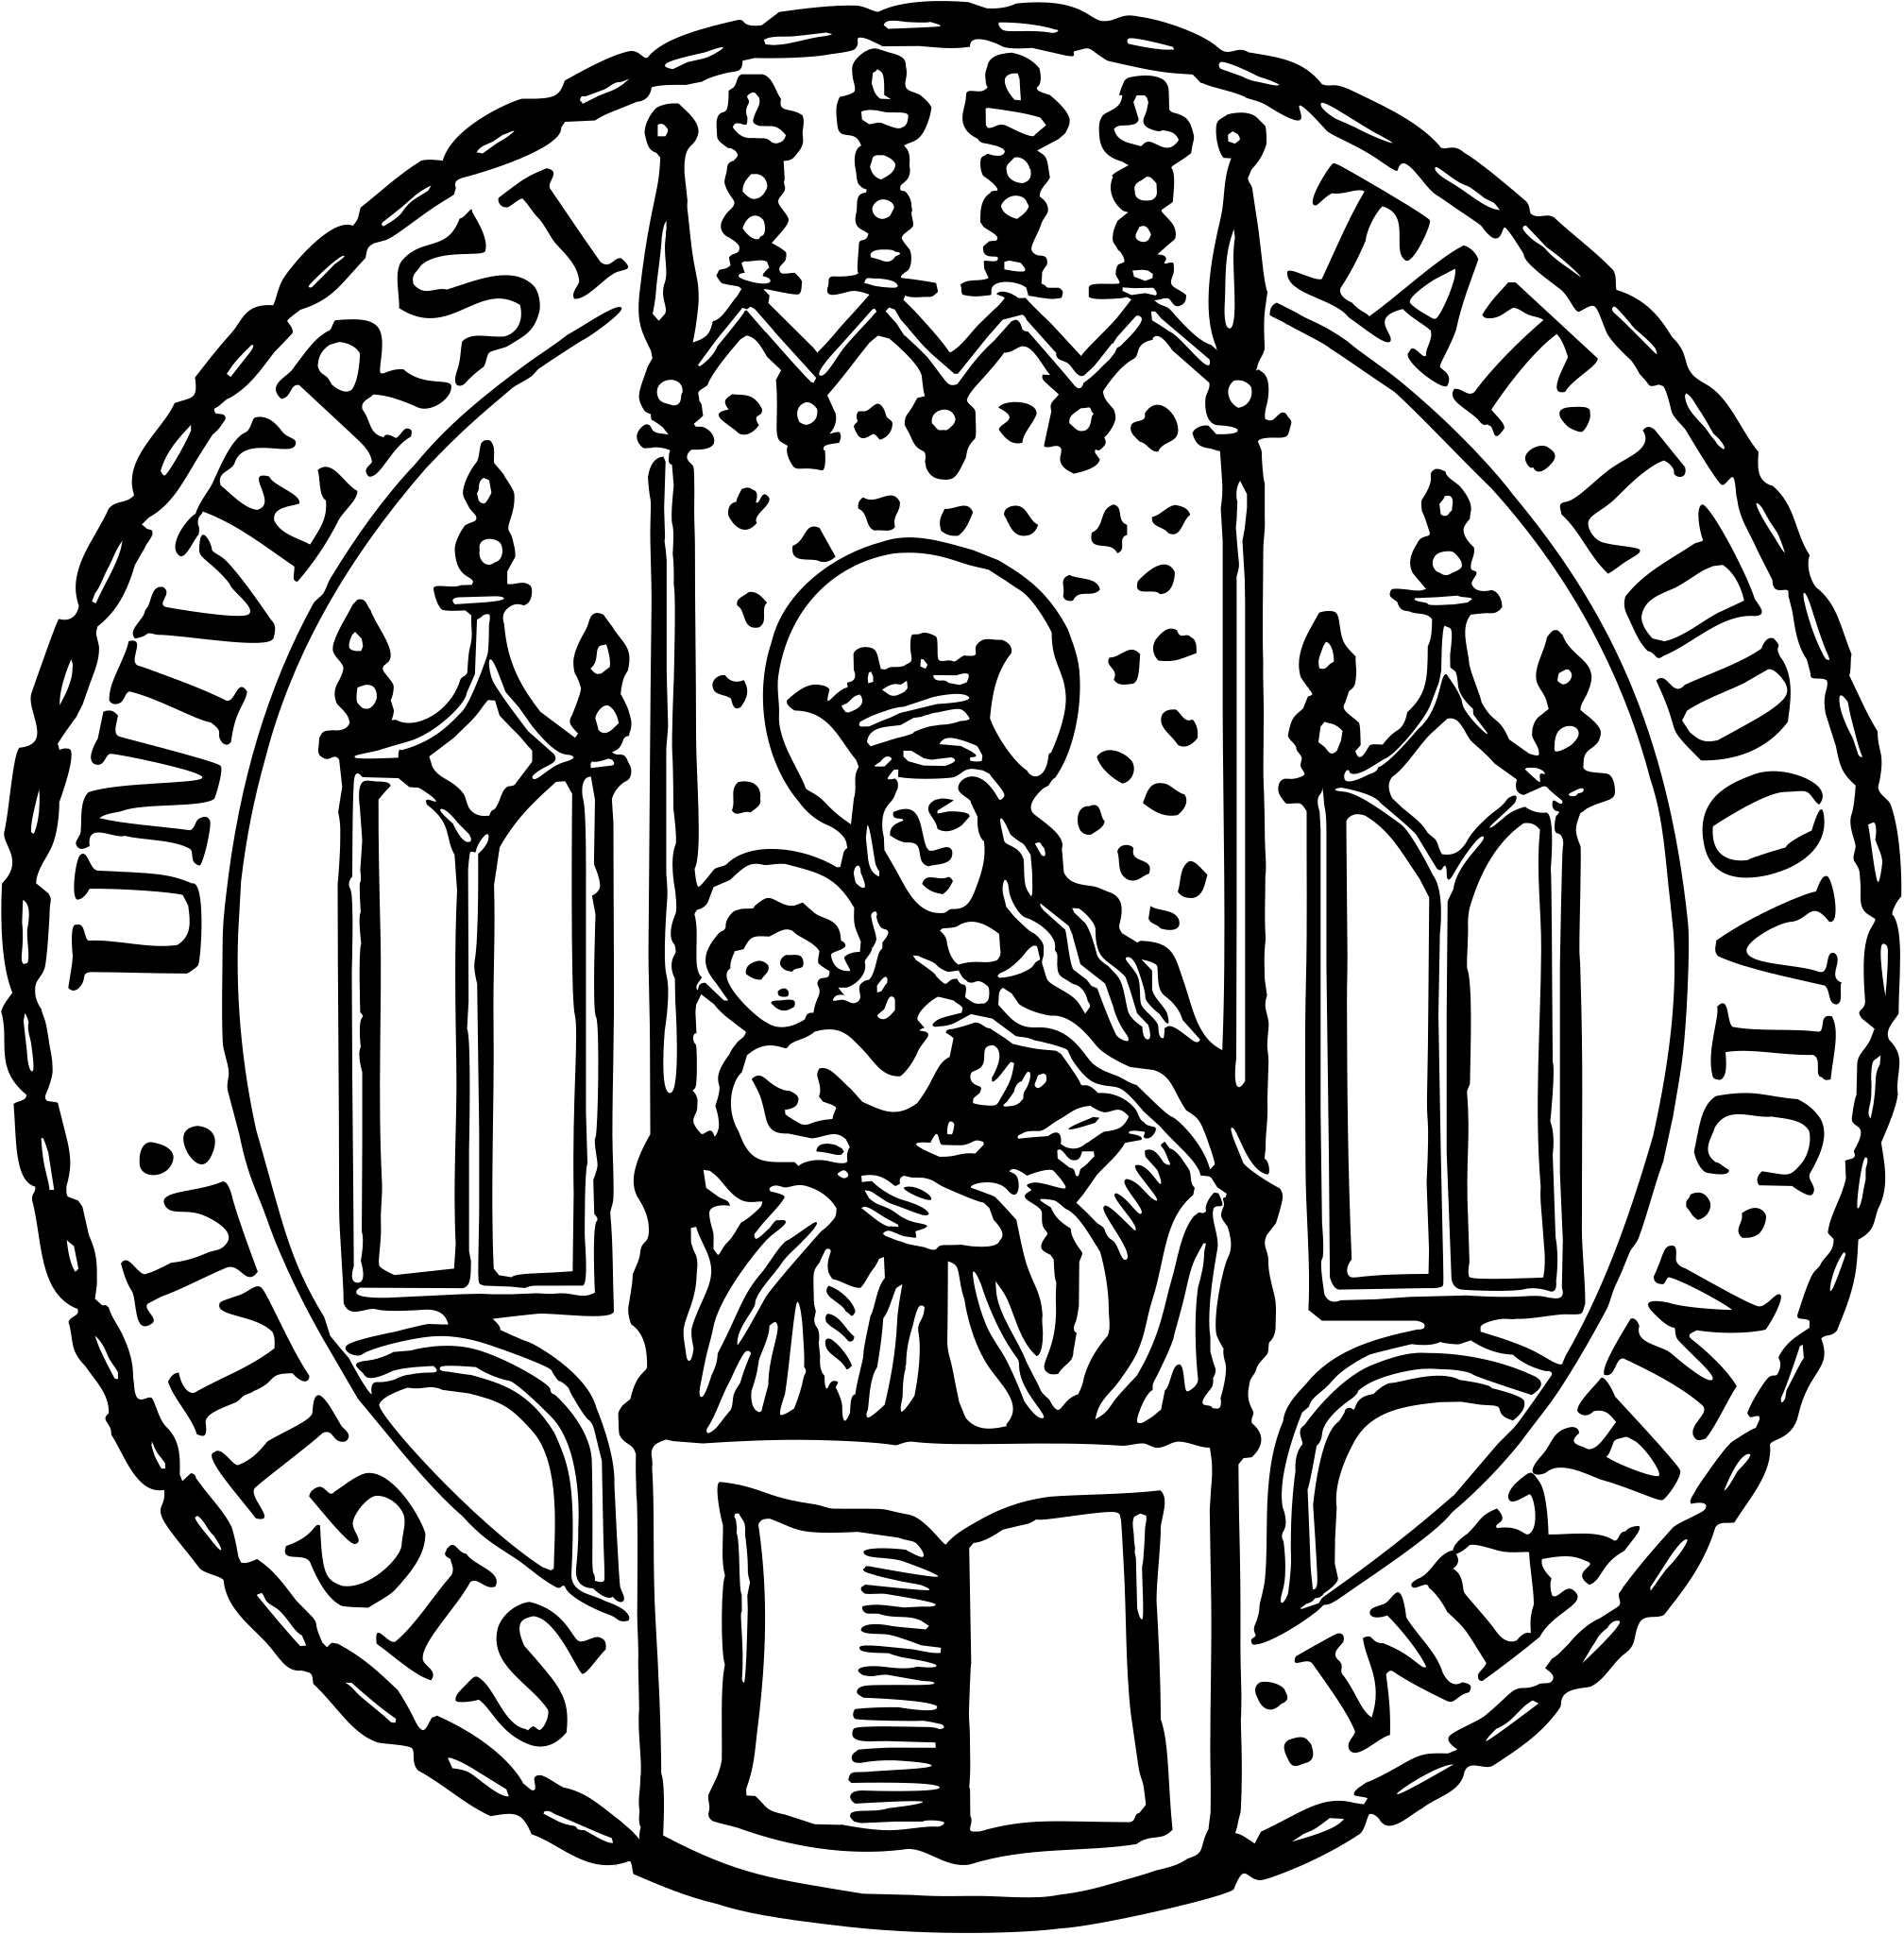
\includegraphics[width=\paperwidth, height=\paperheight, keepaspectratio]{figures/lmu-siegel.png}
%             }
%             \vfill
%         }
%     }
% }
%%%%%%%%%%%%%%%%%%%%%%%%%%%%%%%%%%%%%%

%%% COMMAND FOR PRETTY CODE HIGHLIGHTING %%%
% source: https://tex.stackexchange.com/questions/140166/making-inline-code-printing-pretty?noredirect=1&lq=1
% \newcommand\code[3][]{
%     \tikz[baseline=(s.base)]{
%         \node(s)[
%             rounded corners,
%             fill=blue!5,        % background color
%             draw=gray,          % border of box
%             %text=gray!50!black, % text color
%             inner xsep =3pt,    % horizontal space between text and border
%             inner ysep =0pt,    % vertical space between text and border
%             text height=2ex,    % height of box
%             text depth =1ex,    % depth of box
%             #1                  % other options
%         ]{\mintinline{#2}{#3}};
%     }
% }
%%%%%%%%%%%%%%%%%%%%%%%%%%%%%%%%%%%%%%%%%%%

%%% COMMAND FOR EMPTY PAGE %%%
% source: https://tex.stackexchange.com/questions/34934/add-a-new-empty-page
\newcommand*\NewPage{\newpage\null\thispagestyle{empty}\newpage}
%%%%%%%%%%%%%%%%%%%%%%%%%%%%%%

%%%% XCOLOR COMMAND %%%
%% -- own command for \textcolor{}{} -- %
%\newcommand{\red}[1]{\textcolor{red}{#1}}
%\newcommand{\green}[1]{\textcolor{green!50!black}{#1}}
%\newcommand{\blue}[1]{\textcolor{blue}{#1}}
%\newcommand{\cyan}[1]{\textcolor{cyan}{#1}}
%\newcommand{\purple}[1]{\textcolor{red!75!blue}{#1}}
%\newcommand{\orange}[1]{\textcolor{orange}{#1}}
%\newcommand{\gray}[1]{\textcolor{white!50!black}{#1}}
%%%%%%%%%%%%%%%%%%%%%%%


%%%%%%%%%%%%%%%%%%%%%%
%%% PACKAGE SETUPS %%%
%%% ============== %%% 

%%% BIBLATEX SETUP %%%
% source: https://tex.stackexchange.com/questions/534565/apply-empty-style-to-the-entire-bibliography
\renewcommand{\bibsetup}{\thispagestyle{empty}}
\makeatletter
\patchcmd{\blx@endenv@bibliography}{\endlist}{\endlist\clearpage}{}{}
\makeatother
%%%%%%%%%%%%%%%%%%%%%%

%%% CLASS SETUP %%%
\setcounter{secnumdepth}{3}
\setcounter{tocdepth}{3}
%%%%%%%%%%%%%%%%%%%

%%% CSQUOTES SETUP %%%
% source: https://tex.stackexchange.com/questions/329334/quote-inline-with-italics
\DeclareQuoteStyle[american]{english}
{\itshape\textquotedblleft}
[\textquotedblleft]
{\textquotedblright}
[0.05em]
{\textquoteleft}
{\textquoteright}
%%%%%%%%%%%%%%%%%%%%%%

%%% FANCYHDR SETUP %%% 
\pagestyle{fancy}
\fancyhf{}
\fancyhead[RE]{\normalfont\bfseries\sffamily\leftmark}
\fancyhead[LO]{\normalfont\bfseries\sffamily\rightmark}
\fancyhead[RO,LE]{\thepage}

\fancypagestyle{plain}{%
  %\fancyhf{}
  %\fancyhead[RO,LE]{\thepage}
}

\ChTitleVar{\bfseries\Large\rmfamily}
\ChNameVar{\Large\sffamily}

\makeatletter
\renewcommand\chaptermark[1]{%
  \markboth{%
    \ifnum \c@secnumdepth >\m@ne
      \if@mainmatter
        %\chaptername
      \fi
    \fi
    #1%
  }{}
}

\renewcommand\sectionmark[1]{\markright{\thesection\enspace #1}}
%\renewcommand\subsectionmark[1]{\markright{\thesubsection\enspace #1}}
\makeatother          
%%%%%%%%%%%%%%%%%%%%%%

%%% FONT SETUP %%%
%\renewcommand{\familydefault}{\sfdefault}
%%%%%%%%%%%%%%%%%%

%%% HYPER SETUP %%%
\hypersetup{   
    pdfpagemode = {UseNone},
    pdftitle = {\getTitleEN},
    pdfauthor = {\getAuthor},
    pdflang = {\langEN},
    colorlinks = true,     
    linkcolor = blue,      
    citecolor = violet,
    filecolor = magenta,      
    urlcolor = blue       
}                        
%%%%%%%%%%%%%%%%%%%

%%% LISTINGS SETUP %%%
\definecolor{backcolor}{HTML}{E3E6E8}
% \definecolor{codebasic}{HTML}{000000}

% \definecolor{codered}{HTML}{FF007F}
% \definecolor{codegreen}{HTML}{00FF7F}
% \definecolor{codeblue}{HTML}{007FFF}
% \definecolor{codecyan}{HTML}{10BCEB}
\definecolor{codepurple}{HTML}{7F00FF}
% \definecolor{codelightpurple}{HTML}{7F77FF}
% \definecolor{codeyellow}{HTML}{FFFF00}
% \definecolor{codelightyellow}{HTML}{FFF777}

\definecolor{codegray}{HTML}{5A7296}

\lstset{
    backgroundcolor=\color{backcolor},   
    basicstyle=\ttfamily\footnotesize,
    keywordstyle=\color{codepurple},
    stringstyle=\color{codered},
    commentstyle=\color{codegray},
    numberstyle=\tiny\color{codegray},
    escapeinside={\%*}{*)},               % if you want to add LaTeX within your code
    breakatwhitespace=false,         
    breaklines=true,                 
    captionpos=b,                    
    keepspaces=true,                 
    numbers=left,                    
    numbersep=5pt,                  
    showspaces=false,                
    showstringspaces=false,
    showtabs=false,                  
    tabsize=2
}
%%%%%%%%%%%%%%%%%%%%%



%%% SI SETUPS %%%
\sisetup{locale=US}                     
\sisetup{per-mode=symbol-or-fraction} 
\DeclareSIUnit \au {au}
\DeclareSIUnit \ly {ly}
\DeclareSIUnit \parsec {pc}
\DeclareSIUnit \yr {yr}
%%%%%%%%%%%%%%%%%

%%% SIDECAP SETUP %%%
\sidecaptionvpos{figure}{t}
%%%%%%%%%%%%%%%%%%%%%

%%% TCOLORBOX SETUP %%%
% \definecolor{mygray}{rgb}{0.8,0.8,0.8}
% \tcbset{
%         on line,
%         boxsep = 2pt,
%         left = 0pt,
%         right = 0pt,
%         top = 0pt,
%         bottom = 0pt,
%         colframe = white,
%         colback = mygray
% }
%%%%%%%%%%%%%%%%%%%%%%%%

%%% TIKZ AND PGFPLOTS SETUP %%%
\usetikzlibrary{intersections}
\usetikzlibrary{decorations.pathreplacing, decorations.markings}
\usetikzlibrary{tikzmark}
\pgfplotsset{every axis/.style={scale only axis}, compat=newest}
%%%%%%%%%%%%%%%%%%%%%%%%%%%%%%%

%%% TITLESEC SETUP %%%
% source: https://tex.stackexchange.com/questions/111643/decrease-space-before-and-after-chapter-in-fncychap
\makeatletter
\patchcmd{\@makechapterhead}{\vspace*{50\p@}}{\vspace*{-20\p@}}{}{}
\patchcmd{\@makeschapterhead}{\vspace*{50\p@}}{\vspace*{-20\p@}}{}{}
\patchcmd{\DOTI}{\vskip 80\p@}{\vskip 40\p@}{}{}
\patchcmd{\DOTIS}{\vskip 40\p@}{\vskip 0\p@}{}{}
\makeatother
% \makeatletter
% \titleformat{\chapter}[frame]
%   {\normalfont}{\filright\enspace \@chapapp~\thechapter\enspace}
%   {8pt}{\LARGE\bfseries\filcenter}
% \titlespacing*{\chapter}
%   {0pt}{0pt}{20pt}
% \makeatother
%%%%%%%%%%%%%%%%%%%%%%

%%% TOC SETUP %%%
% source: https://tex.stackexchange.com/questions/5787/table-of-contents-with-page-style-empty
\AtBeginDocument{\addtocontents{toc}{\protect\thispagestyle{empty}}}
%%%%%%%%%%%%%%%%%

\addbibresource{sources/bib_thesis.bib}

\begin{document}

%%%%%%%%%%%%%%%%%%%%
%%% FRONT MATTER %%%
%%% ============ %%%

\frontmatter

%%% FRONTPAGE
\begin{titlepage}   

    \vspace*{\stretch{1}}
    {\parindent0cm
    \rule{\linewidth}{.4ex}}  
  \begin{center}
    \vspace*{\stretch{0.4}}
    {\sffamily \bfseries \Huge \getTitleEN \par}
    \vspace*{\stretch{0.4}}
  \end{center}
    \rule{\linewidth}{.4ex}
    \vspace*{\stretch{3}}
  

  \begin{center}
    % {\rmfamily \bfseries \Large Bachelor Thesis}

    \vspace*{\stretch{0.3}}


  \begin{figure}[!h]
    \centering
    \transparent{0.2}
    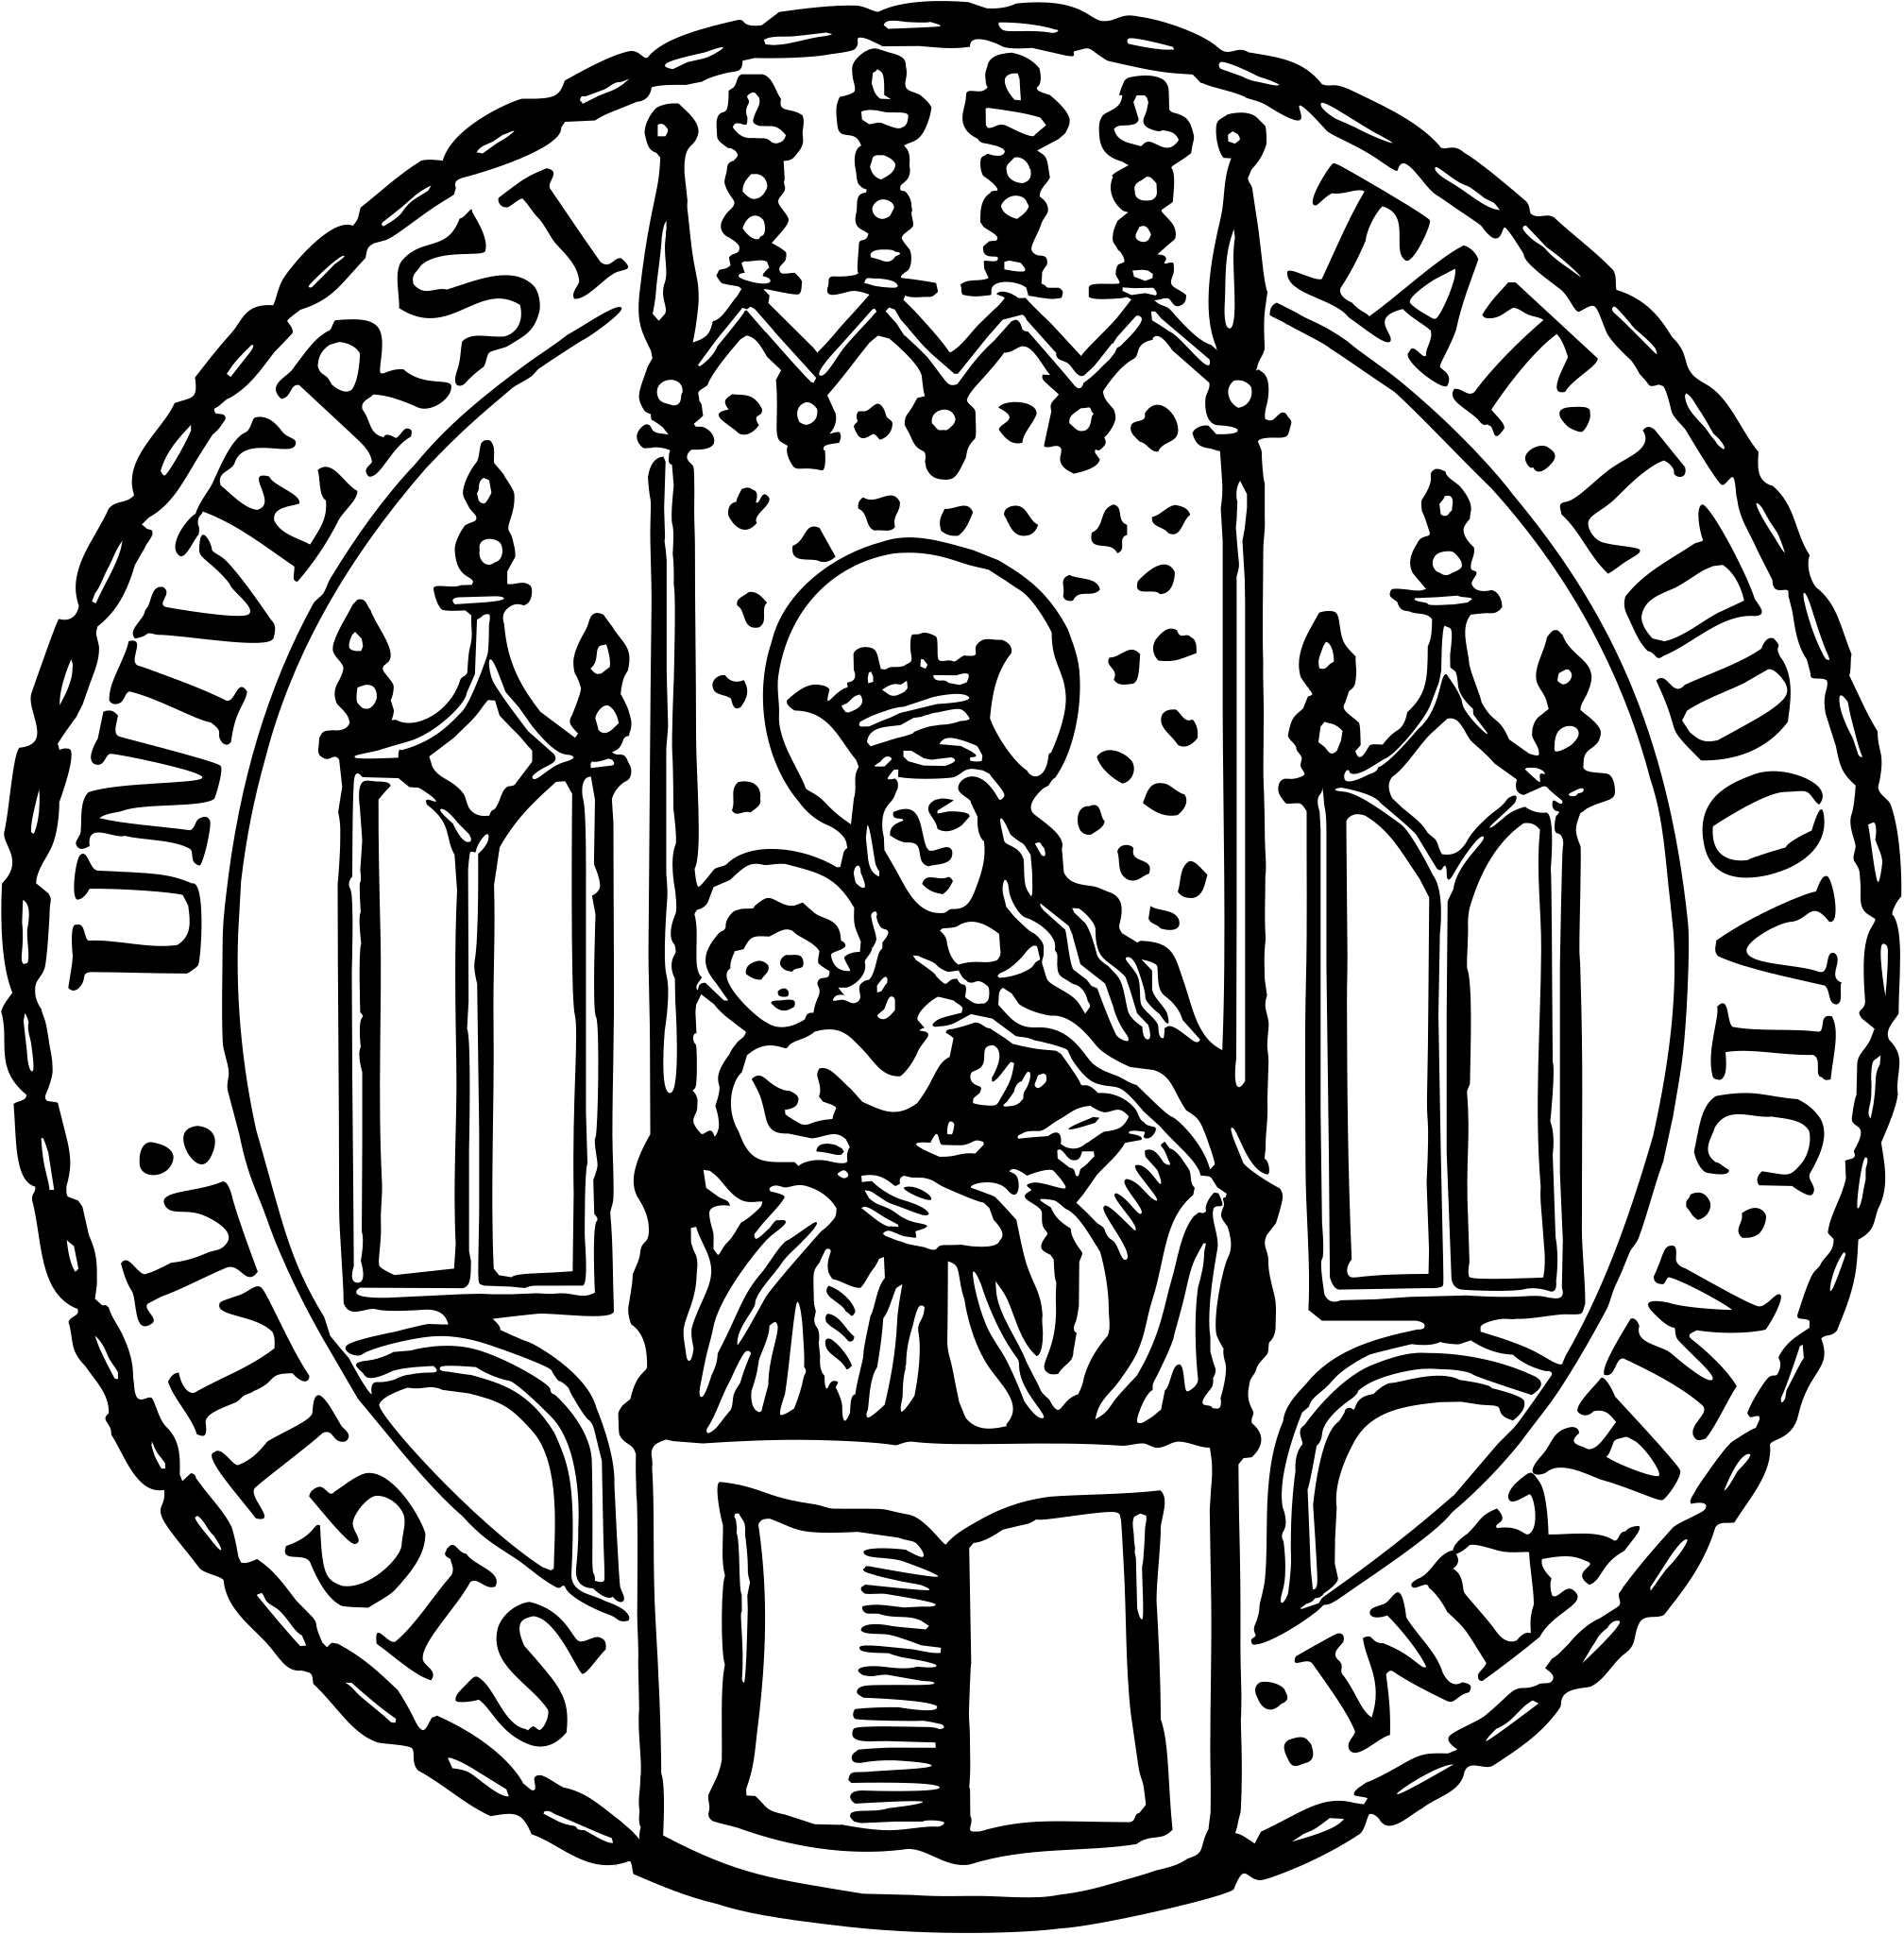
\includegraphics[scale=0.15]{figures/lmu-siegel.png}
  \end{figure}
  

    \vspace*{\stretch{2}}
     {\scshape \large
    %  University Observatory Munich \\
    %  Fakulty of Physics \\
    %  at the Ludwig-Maximilians-University \\
    %  Munich

     \vspace*{\stretch{1}}

     submitted by \\

     \vspace*{\stretch{0.3}}
     {\rmfamily \bfseries \Large \getAuthor} \\


     \vspace*{\stretch{2}}
     %\getPrintLocationEN, \getSubmissionDateEN
     }
  \end{center}
  
  %\AddToShipoutPicture*{\BackgroundPic}

\end{titlepage}

\thispagestyle{empty}

%%% TITLEPAGE 
\begin{titlepage}   

    \vspace*{\stretch{1}}
    {\parindent0cm
    \rule{\linewidth}{.4ex}}
  \begin{center}
    \vspace*{\stretch{0.4}}
    {\sffamily \bfseries \Huge \getTitleDE \par}
    \vspace*{\stretch{0.4}}
  \end{center}
    \rule{\linewidth}{.4ex}
    \vspace*{\stretch{3}}


  \begin{center}
    {\rmfamily \bfseries \Large Bachelorarbeit}

    \vspace*{\stretch{0.3}}

    {\scshape \large
     Universitätssternwarte München \\
     Fakultät für Physik \\
     an der Ludwig-Maximilians-Universität \\
     München
     
     \vspace*{\stretch{1}}
     
     vorgelegt von \\
    
     \vspace*{\stretch{0.3}}
     {\rmfamily \bfseries \Large \getAuthor} \\

     
     \vspace*{\stretch{2}}
     \getPrintLocationDE, \getSubmissionDateDE
     }
  \end{center}
  
\end{titlepage}

\thispagestyle{empty}
\begin{titlepage}   

    \vspace*{\stretch{1}}
    {\parindent0cm
    \rule{\linewidth}{.4ex}}  
  \begin{center}
    \vspace*{\stretch{0.4}}
    {\sffamily \bfseries \Huge \getTitleEN \par}
    \vspace*{\stretch{0.4}}
  \end{center}
    \rule{\linewidth}{.4ex}
    \vspace*{\stretch{3}}
  

  \begin{center}
    {\rmfamily \bfseries \Large Bachelor Thesis}

    \vspace*{\stretch{0.3}}

    {\scshape \large
     University Observatory Munich \\
     Fakulty of Physics \\
     at the Ludwig-Maximilians-University \\
     Munich

     \vspace*{\stretch{1}}

     submitted by \\

     \vspace*{\stretch{0.3}}
     {\rmfamily \bfseries \Large \getAuthor} \\


     \vspace*{\stretch{2}}
     \getPrintLocationEN, \getSubmissionDateEN
     }
  \end{center}
  
\end{titlepage}

\thispagestyle{empty}

%%% SUPERVISORS
\thispagestyle{empty}

\vspace*{\stretch{1}}

\begin{flushleft}
    {\large
     First supervisor:  \getSupervisorOne \\[1mm]
     Second supervisor: \getSupervisorTwo \\
     }
\end{flushleft}

\cleardoublepage{}

\thispagestyle{empty}

%%% ACKNOWLEDGEMENT
% \chapter*{Danksagung}
\phantomsection\addcontentsline{toc}{chapter}{\protect Danksagung}

\noindent Es war ein langer Weg, bis ich endlich diesen Punkt in meinem Leben erreicht habe. Es war nicht einfach. Aber niemand sagte, dass das Leben einfach wird.

\noindent Ich war etwa 12 Jahre alt, als ich das erste Mal mit meinem kleinen Teleskop Ausschau nach dem schönsten Objekt unseres Sonnensystem hielt. In der Lage zu sein, die Ringstruktur des Saturn zu bewundern, öffnete mir die Augen und das Herz zur Erkundung der Schönheit der Natur - der Schönheit des Weltraums.

Während wir aufwachsen, versuchen wir - getrieben von Neugier und Faszination - die Welt um uns herum zu verstehen. Wir sind auf der Suche nach Antworten auf die ``großen Fragen des Lebens''.

\noindent Woher kommen wir ? \\
Warum ist das Universum entstanden ? \\
Wie alt ist das Universum ? \\
Welche Mechanismen bestimmen die Geschicke der Welt ? \\
Was wird in der Zukunft passieren ? \\
Welche Rolle spiele ich in diesem unvorstellbar großen Universum ? \\
Welchen Sinn hat mein Leben ? \\
Und, wohin möchte ich gehen ? 

\noindent Das sind gewiss keine einfachen Fragen. Und das ist wahrscheinlich auch der Grund, warum dies die ältesten Fragen der Menschheit sind. \\
Im Laufe meiner ``Reise durch das Leben'' versuchte ich, Antworten auf diese Fragen zu finden. Vielleicht schaffe ich es, auf einige dieser Fragen mögliche Antworten in dieser Arbeit geben zu können. Vielleicht werde ich auf einige dieser Fragen nie eine Antwort finden.
Aber zumindest auf die Frage nach dem Sinn \textit{meines} Lebens habe ich eine Antwort gefunden: die Schönheit der Natur zu entdecken. Und während dieses Abenteuers niemals aufzugeben - egal, wie hart und frustrierend das Leben manchmal sein kann. Egal, wie oft ich gefallen bin oder noch auf den harten Boden der Realität fallen werde. Denn es ist meine Neugier, meine Ambition und meine Leidenschaft, welche mich dazu bringt, wieder aufzustehen und meine Augen, meinen Blick in den Himmel zu richten.

\noindent Das ist wohl die wichtigste Lektion, welche ich in den letzten Jahren im Laufe des Physikstudiums gelernt habe.

\noindent Die Tatsache, es so weit gebracht zu haben, ist jedoch nicht nur dem Lesen von Lehrbüchern, dem Rechnen von Übungsblättern oder dem Vorbereiten auf Klausuren geschuldet. Denn es ist nicht nur der Fleiß, den ich erbracht habe.
Ich stehe, wo ich bin, dank dem Fleiß bestimmter Menschen, die in mein Leben kamen. Ich bin äußert dankbar, dass ich das Glück hatte, jene Menschen zu begegnen. Und nun ist wohl der beste Anlass, um ihnen meinen herzlichsten Dank mitzuteilen.

\noindent In erster Linie möchte ich meinen Lehrern danken, welche mir nicht nur viel beibrachten, sondern auch ihr Bestes gaben, um auf meine schwierigen Fragen Antworten zu finden und meine Wissensbegierde zu stillen, was wahrscheinlich nicht immer einfach war und viel Geduld erforderte,



\chapter*{Acknowledgement}
\phantomsection\addcontentsline{toc}{chapter}{\protect Acknowledgement}
\thispagestyle{empty}

\epigraph{\textit{``The effort to understand the universe is one of the very few things which lifts human life a little above the level of farce and gives it some of the grace of tragedy.''}}{Steven Weinberg, \cite[Epilogue]{Weinberg1993}}

\noindent It was a long path to finally achieve this point in my life. And it was not an easy one. But no one said that life was going to be easy.

\noindent I was about 12 years old when I watched the sky the very first time with my telescope, looking out for the most beautiful planet of our solar system. Being able to admire the ring structure of Saturn opened my eyes and my heart to explore the beauty of nature, the beauty of space. \\

\noindent While growing up, we try, driven by curiosity and fascination, to understand the world around us. We may seek answers to ``the big questions of life''. \\ 

{ \itshape
\noindent Where do we come from? \\
Why did the universe come to existence? \\
How old is the universe? \\
Which mechanisms in nature guide the course of all events? \\
What will happen in the future? \\
Which role do I play in this unimaginable big universe? \\
What is the purpose of my life? \\
And, where do I want to go? \\
}

\noindent Those are difficult questions. And that is why those questions are probably the oldest ones of humanity. \\
Throughout my ``journey of life'', I tried to find answers to those questions. Maybe I could find some attempts to answer a few of those in this thesis. Maybe I will never find an answer to some of these questions. \\

\noindent At least I found an answer what the purpose of \textit{my} life is: to discover the beauty of nature. Going on with my journey, trying to find answers. And never giving up during this adventure -- no matter, how hard and how frustrating life can be sometimes. No matter how often I have fallen or I will fall down to the harsh ground of reality. Because it is my curiosity, my ambition and my passion that makes me standing up again to turn my eyes, my gaze into the sky. \\ 

\noindent That is the most important lesson I have learned in the last years, studying physics. \\ 

\noindent The fact that I made it so far is not only through reading textbooks, doing my exercise sheets or preparing for exams. Because it is not only the effort I brought up. \\
I am where I am thanks to the effort of several people that came into my life. I am very glad that I had the luck to get to know these people. And therefore, this is the best occasion for me to thank them. \\

\noindent First of all, I want to thank my teachers, who not only taught me a lot, but also did their best to answer my difficult questions and quench my thirst for knowledge, which was probably not always easy and took a lot of patience, \\

\noindent {\bfseries Pierette Al-Korey, Ulrike Blattert, Peter Bodden, Nicole Bömecke, Jörg Bühler, Reiner Büter, Rolf Heckmann, Petra Jähnigen, Thomas Schröder Klementa, Axel Knuth, Eva Krüger, René Meyer-Brede, Angelika Nieboer, Roland Petereit, David Stephan, Volkhard Stierhof, Stefan Usée, Selma Weiß-Tümmers, Wolf Wingenfeld, Sema Yilmaz, Mike Ziegner.} \\

\noindent Further, I want to thank my supervisors \textbf{Jochen} and \textbf{Steffen}, who offered me this opportunity to write my thesis on cosmology and kindly assisted me at any time with my questions. \\

\noindent I want to thank \textbf{Silas}, who provided me his bachelor thesis on a similar topic, with which I was able to compare the results I obtained during my analysis and evaluations. \\

\noindent I would like to thank all my colleagues, fellow students and friends whom I have met and who accompanied me on my way through the bachelor studies and always stood by me -- especially to \textbf{Arthur} and \textbf{Marc}, who can bring a smile to my face even on the saddest days. \\

\noindent I want to thank \textbf{Yannick}, not only for his advice on how to reduce the computation time of my codes from several hours to a few seconds and proofreading this thesis, but for being a good friend. \\

\noindent My heartfelt thanks goes to \textbf{Simon} -- the most kind-hearted person I have ever met. By submitting this bachelor thesis, I would like to fulfill my promise to him to never give up my bachelor studies and successfully achieve the bachelor's degree in physics. \textbf{Thank you Simon}. \\

\noindent And last but not least, I would like to express my greatest gratitude to my family -- especially \textbf{my father}, \textbf{my mother} and \textbf{my sister}, who raised me and cared for me since the day I was born, who provided me everything that was needed to enjoy an excellent education, who opened the path on my way to a self-determined life and contributed to becoming the person I am today. \\

\noindent From the bottom of my heart -- thank you.

\thispagestyle{empty}

%%% MEMORY
\thispagestyle{empty}

\vspace*{0.5\textheight}

\begin{center}
    \itshape In loving memory of Simon Jacob Gallo and Gamal Tadros Mishreky 
\end{center}


\thispagestyle{empty}

%%% NOTATION AND CONVENTIONS
\chapter*{Notation and conventions}
\phantomsection\addcontentsline{toc}{chapter}{\protect Notation and conventions}
\thispagestyle{empty}

Throughout this thesis, we choose the signature for the metric of spacetime to be \\
${\eta_{\mu\nu} = \diag(-,+,+,+)}$.
This is a list of books on astrophysics, cosmology and general relativity I have came across while working on this thesis, divided into the different sign convention for the metric of spacetime. 
\begin{itemize}
    \item[$(\bs{+})$] $\eta_{\mu \nu} = \diag(-,+,+,+)$
    \begin{itemize}
        \item[$\bullet$] Matthias Bartelmann. \textit{Das kosmologische Standardmodell} \cite{Bartelmann2019}
        \item[$\bullet$] Sean M. Carroll. \textit{Spacetime and Geometry} \cite{SeanCarroll2019}
        \item[$\bullet$] Scott Dodelson, Fabian Schmidt. \textit{Modern Cosmology} \cite{Dodelson2020}
        \item[$\bullet$] C.W. Misner, K.S. Thorne, J.A. Wheeler. \textit{Gravitation} \cite{MTW2017}
        \item[$\bullet$] Bernard Schutz. \textit{A First Course in General Relativity} \cite{Schutz2009}
        \item[$\bullet$] Karl-Heinz Spatscheck. \textit{Astrophysik} \cite{Spatschek2017}
        \item[$\bullet$] Steven Weinberg. \textit{Cosmology} \cite{Weinberg2008}
        \item[$\bullet$] A. Zee. \textit{Einstein Gravity in a Nutshell} \cite{Zee2013}
    \end{itemize}
    \item[$(\bs{-})$] $\eta_{\mu \nu} = \diag(+,-,-,-)$
    \begin{itemize}
        \item[$\bullet$] Bradley W. Carroll, Dale A. Ostlie. \textit{An Introduction to Modern Astrophysics} \cite{BradleyCarroll2007}
        \item[$\bullet$] Viatcheslav Mukhanov. \textit{Physical Foundations of Cosmology} \cite{Mukhanov2005}
        \item[$\bullet$] P.J.E. Peebles. \textit{Principles of Physical Cosmology} \cite{Peebles1993}
    \end{itemize}
\end{itemize}

\noindent In order not to lose the connection between empirically measured quantities we can observe and theoretical quantities introduced by the cosmological models, we choose to let $c = \SI{299 792 458}{\meter/\second}$ and $G = \SI{6.674e-11}{\meter^3/(\kilogram \ \second^2)}$ in SI-units.\footnote{... although the convenience for mathematical manipulations in the case of natural units where $c = G = 1$ cannot be denied.}

\thispagestyle{empty}

%%% ABSTRACT
\chapter*{Abstract}
\phantomsection\addcontentsline{toc}{chapter}{\protect Abstract}

Here you can write a summary, what your thesis is about or short introduction to your thesis.

\bt

\thispagestyle{empty}

%%% TABLE OF CONTENT
\pdfbookmark{\contentsname}{Contents}
\tableofcontents 
\clearpage


%%%%%%%%%%%%%%%%%%%%
%%% MAIN MATTER %%%%
%%% =========== %%%%

\mainmatter

%%% INTRODUCTORY CONCEPTS OF ASTROPHYSICS
\chapter{Introductory Concepts of Astrophysics}
\label{chap:introductory-concepts-of-astrophysics}
\thispagestyle{empty}

In 2011, Saul Perlmutter, Adam G. Riess, and Brian P. Schmidt received the Nobel Prize in Physics \enquote{for the discovery of the accelerating expansion of the Universe through observations of distant supernovae}. \footnote{Press release: \href{https://www.nobelprize.org/prizes/physics/2011/press-release/}{https://www.nobelprize.org/prizes/physics/2011/press-release/}} \\
Since then, we know that the expansion of the universe is accelerating.
The cause of this accelerated expansion is still unknown, but there are some theoretical models which attempt to explain this phenomenon. \\

\noindent The established model in recent cosmology is the \textbf{$\Lambda$CDM-model}, sometimes referred as the \textit{standard model of cosmology}.
In this model, the cause of the accelerated expansion is due to the so called \textit{cosmological constant} $\Lambda$, which appears as a physical constant in Einstein's field equations of general relativity like the Newtonian gravitational constant $G$. \\

\noindent Another model, published in April 2000 by Gia Dvali, Gregory Gabadadze and Massimo Porrati, -- the \textbf{DGP-model} -- proposes a modification of Einstein's field equations by introducing a fifth dimension to the four-dimensional spacetime, so that gravity behaves equivalently to Newtonian gravity on small distances, but weakens on large scales. \\


\noindent Before going into details about both cosmological models, let me introduce relevant concepts in physics and astronomy from which we can relate measurable physical quantities, like the brightness of stars or their redshift, to more abstract properties of the universe like its scale factor. Based on certain assumptions of a theory, it is possible to develop models that make predictions about properties of the universe, for example, how the expansion and its evolution in time influences the relation of physical quantities.



\section{Distance Measurement in Astronomy}

Essential to astronomical observations and measurements is to determine the distance to objects in space like stars, star clusters, galaxies or even clusters of galaxies. \\
By looking at night into the sky, the only information perceived by our human eye are the brightness and some color in which objects (mostly stars) appear.
How do we determine the distance to those objects?


\subsection{The Parallax Method}

One method to determine the distance to an object is by using the \textit{parallax effect}. \\
For this method, we assume that the observed object is almost stationary relative to earth.
First, we detect the position of the measured object in the sky. After a while (for example, after a half year), the object appears at a slightly different position in the sky, since earth moved on its elliptical orbit which leads to another point of view for the observation.
\begin{figure}[H]
    \centering
    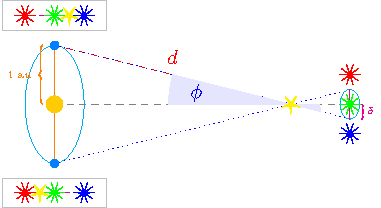
\includegraphics[scale=1.8]{figures/tikz/parallax/parallax.pdf}
    \caption{To determine the distance $d$ between earth and the yellow star, we consider the small change of the position $\delta$ around the green star under which the yellow star appears. The difference $\delta$ relates to the angle $\phi$.}
    \label{fig:parallax}
\end{figure}
\noindent By measuring the appeared difference $\delta$ of the object's position and relating this difference to the angle $\phi$ under which the object changed its position in the sky, we can calculate the distance $d$ by 
\begin{align}
    d = \frac{\SI{1}{\au}}{\sin(\phi)} \approx \frac{\SI{1}{\au}}{\phi},
\end{align}
where $\SI{1}{\au} \approx \SI{149.6e+9}{\meter}$ (``astronomical unit''\footnote{Since 2012, the astronomical unit was redefined by the IAU (International Astronomical Union) to be exactly $\SI{1}{au} := \SI{149597870700}{\meter}$, see \textit{Resolution B2} at the XXVIII General Assembly of IAU: \href{https://www.iau.org/static/resolutions/IAU2012\_English.pdf}{https://www.iau.org/static/resolutions/IAU2012\_English.pdf}}) is defined as the average distance $d_{\earth \odot}$ of earth to the sun. \\ 
The small-angle approximation can be considered justified, since the distance to earth nearest star (beyond of our solar system), Proxima-Centauri, is about $d_{\text{P.C.}} \approx \SI{4.2}{\ly}$ and therefore $\phi_{\text{P.C.}} \approx \arcsin \bigl( \frac{\SI{1}{\au}}{\SI{4.2}{\ly}} \bigr) \approx \SI{3.723e-6} \ll 1$.
The larger the distance to the measured object, the smaller the angle is. \\
\noindent Since the parallax method is one of the most important ways to measure the distance of far away objects, we define the distance of a \textit{parsec} (``parallax second'') as the distance to an object, under which the parallax is $\phi = \SI{1}{\arcsec} = \frac{1}{3600} \SI{}{\degree}$:
\begin{align}
    \SI{1}{\parsec} := \frac{\SI{1}{\au}}{\sin \bigl( \frac{1}{3600} \SI{}{\degree} \bigr)} \approx \SI{3.26}{\ly} \approx \SI{3.086e16}{\meter}.
\end{align}

\noindent This is the usual unit by which cosmological distances or parameters are expressed, for example the \textit{Hubble constant} $H_{0} \approx \SI{67.66}{\frac{\kilo \meter}{\second} \mega \parsec^{-1}}$.\footnote{The value of $H_{0}$ according to the results of the \textit{Planck Collaboration 2018}, \cite[Table 7]{Planck2020} } \\ 

\noindent We should keep in mind that this method has of course boundaries and is practically useful for the local region of our galaxy, since the larger the distance to an observed object is, the apparent change in position in the sky gets smaller and is almost unnoticable for objects with a distance on cosmological scale ($d \gtrsim \SI{300}{\mega \parsec}$). 

\subsection{The Distance Modulus}

Another method to determine the distance to an object with a certain luminosity $L$ is to measure its radiant flux $F$ at a distance $d$ by
\begin{align}
    F = \frac{L}{4\pi d^2}. \label{eq:radiant-flux} 
\end{align}
In general astronomical observations, it is not the radiant flux of a star that is measured. Rather, we observe \textit{differences} of brightness or magnitude $m$ between two objects. We define a difference in magnitude between two objects $m_{1} - m_{2} =: \Delta m$ so that the radiant flux $F_{2}$ of object 2 is 100 times higher than the radiant flux $F_{1}$ of object 1 when their difference in magnitude is $\Delta m = 5$, so 
\begin{align}
    \frac{F_{2}}{F_{1}} = 100 \Leftrightarrow m_{1} - m_{2} = \Delta m = 5.
\end{align}
This leads us to the relation between the difference of magnitude $\Delta m$ and the relation of the radiant flux of two objects
\begin{align}
    \frac{F_{2}}{F_{1}} = 100^{\frac{m_{1} - m_{2}}{5}} 
\end{align}
and therefore with Equation \eqref{eq:radiant-flux}
\begin{align}
    m_{1} - m_{2} = \frac{5}{2} \log_{10} \biggl( \frac{F_{2}}{F_{1}} \biggr) = \frac{5}{2} \log_{10} \biggl( \frac{L_{2}}{4\pi d_{2}^2} \frac{4\pi d_{1}^2}{L_{1}} \biggr) = \frac{5}{2} \log_{10} \biggl( \frac{L_{2}}{L_{1}} \biggr) + 5 \log_{10} \biggl( \frac{d_{1}}{d_{2}} \biggr). \label{eq:rel-magnitude-distance-relation} 
\end{align}
So, calculating the distance to one of both objects, for example object 2, would require us to know their \textit{relative} magnitudes $m_{1}$ and $m_{2}$, their luminosities $L_{1}$ and $L_{2}$ and the distance $d_{1}$ to object 1. \\
To eliminate the need of knowing five quantities, we can define an \textit{absolute} magnitude $M$ as the magnitude an object would have at a distance of $d = \SI{10}{\parsec}$. If we consider only one object, we therefore can calculate the distance to this object by
\begin{align}
    m - M = \frac{5}{2} \underbrace{\log_{10} \biggl( \frac{L}{L} \biggr)}_{ = 0} + 5 \log_{10} \biggl( \frac{d}{\SI{10}{\parsec}} \biggr) = 5 \log_{10} \biggl(\frac{d}{\SI{10}{\parsec}}\biggr). \label{eq:distance-modulus} 
\end{align}
We call the difference between the relative magnitude $m$ and the absolute magnitude $M$ of one object its \textit{distance modulus}. \\
The benefit of the distance modulus is that we only have to know two quantities, $m$ and $M$, to calculate the distance to an object. \\
Unfortunately, we cannot measure the absolute magnitude $M$ of an object that easily (since we cannot fly to far away stars and measure the observed magnitude or radiant flux at a distance of $\SI{10}{\parsec}$ to them), which is why we rely on Equation \eqref{eq:rel-magnitude-distance-relation}.
However, we could reduce the amount of unknown variables by calibrating the relation \eqref{eq:rel-magnitude-distance-relation} with an object which luminosity and distance is known. \\

\noindent One could choose to calibrate Equation \eqref{eq:rel-magnitude-distance-relation} by measuring the properties of the nearest star to earth -- our sun. Given the magnitude $m_{\odot}$, the luminosity $L_{\odot}$ and the distance to sun $d_{\earth \odot} = \SI{1}{au}$, we obtain 
\begin{align}
    m = m_{\odot} - \frac{5}{2} \log_{10} \biggl(\frac{L}{L_{\odot}}\biggr) + 5 \log_{10} \biggl(\frac{d}{\SI{1}{au}}\biggr). 
\end{align}

\noindent By this calibration, we could determine the distance to an observed object, if we knew its luminosity $L$ and measured its relative magnitude $m$. Generally, the luminosity of objects like stars could varying arbitrarily. To obtain a reliable distance measurement, we are looking for objects whose luminosity can be predicted very precisely -- so called \textit{standard candles}. \\



\subsection{Possible Candidates for Standard Candles} 

Generally, there are two established candidates for standard candles in astronomy. Since we deal in this thesis with data of type Ia supernovae, the focus lies on the second paragraph of this subsection. For the sake of completeness, however, the cepheids as possible standard candles should not be unmentioned -- also to emphasize why we rely on supernovae of type Ia to determinine cosmological distances.

\subsubsection{Cepheids}

There are several types and classes of cepheids, but they all have in common that those stars obey a certain, periodic relation of luminosity and time. \\

\noindent Without going into details\footnote{For further information and more detailed explanation how stellar pulsation and its underlying $\kappa$-mechanism can be calculated, I recommend chapter 14 ``\textit{Stellar Pulsation}'' in \cite{BradleyCarroll2007}.} the periodicity of luminosity is caused by fluctuations of temperature dependent opacity in the stars photosphere due to transitions between single- and dual-ionized Helium inside the star. 

\noindent It is important to identify cepheids of the same type -- cepheids that share the same physical properties, like their metalicity or the same periodicity pattern in their luminosity, to ensure that the same physical process is occuring in all cepheids of a certain type.
\noindent From then on, it is possible to determine the luminosity of all cepheids of the same type by observing one cepheid, measuring its relative magnitude $m$ and its distance $d$ by the parallax method. \\

\begin{figure}[H]
    \centering
    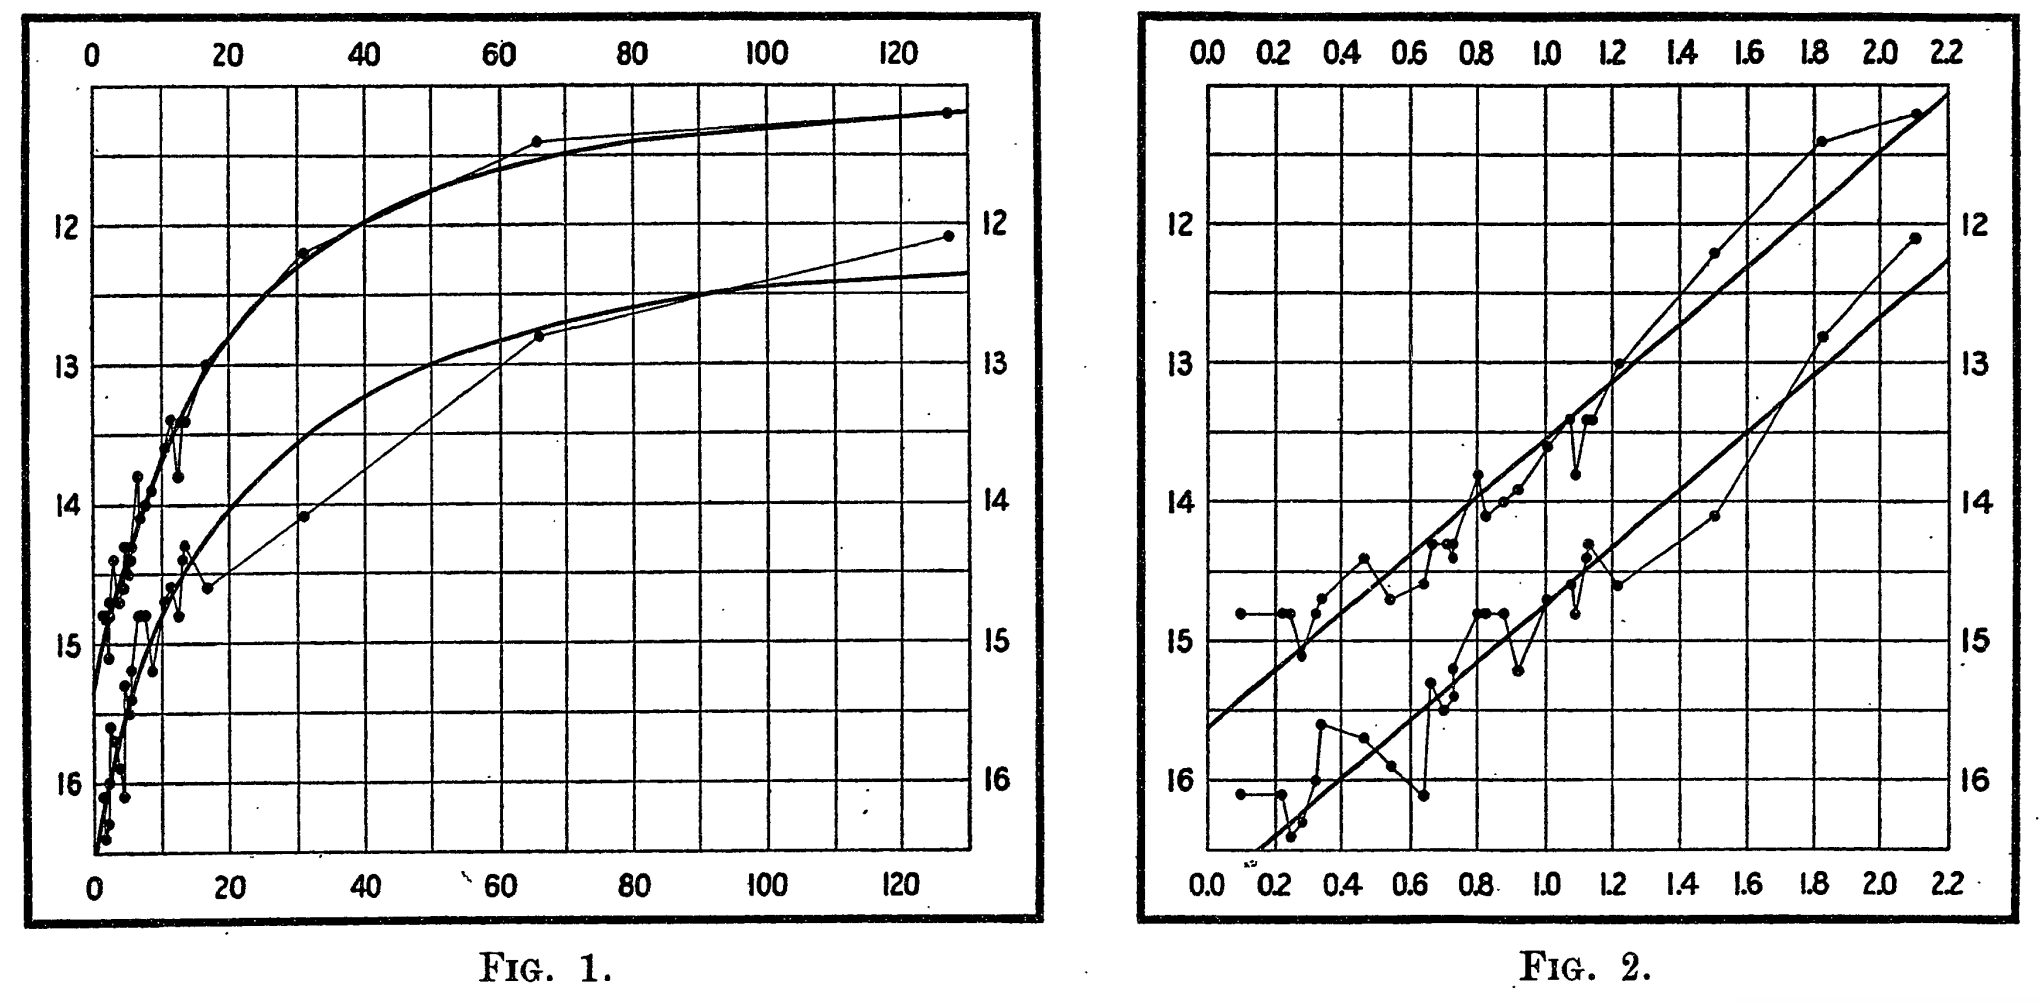
\includegraphics[scale=0.3]{figures/images/leavitt_period-luminosity.png}
    \caption{First observed direct, logarithmic periodicity between time ($x$-axis in days) and magnitude ($y$-axis) of 25 stars in the Small Magellanic Cloud by Henrietta Leavitt, published 1912. Source: \cite{Leavitt1912}.}
\end{figure}


\noindent However, in order to use cepheids for distance determination, they must first be observed and resolved.
Even with our most powerful telescopes that we have today, resolution of cepheids is only possible in our local, galactic neighborhood, for example in the Large Magellanic Cloud or the Andromeda Galaxy. Therefore, the boundary to resolute cepheids in other galaxies is currently about $\sim \SI{30}{\mega \parsec}$ (\cite[p.~47]{Bartelmann2019} and \cite[p.~3]{Engelmann2013}). \\
For larger scales, we need much brighter standard candles.



\subsubsection{Supernovae of Type Ia}

In general, supernovae are abrupt bursts of luminosity from massive stars, often accompanied by explosive thermonuclear reactions.
While supernovae of type Ib, Ic and II occur due to an imbalance between the star's gravity, which causes its nucleus to collapse, and radiation emitted by nuclear fusion inside the star, which pushes against its photosphere, supernovae of type Ia are caused by a white dwarf accreting a companion star and therefore increasing in mass. \\
If, due to accreating a companion star, the white dwarf reaches a mass limit over $\sim 1.4 M_{\odot}$ (where $M_{\odot} \approx \SI{1.98e+30}{\kilogram}$ is the mass of the sun, \cite[p.~48]{Bartelmann2019}), which is called the \textit{Chandrasekhar limit} $M_{\text{Ch}}$, the nucleus of the white dwarf beocmes unstable, since the degeneracy pressure of the electrons (Pauli exclusion principle) cannot resist the gravitational forces any more. \\
Inside the white dwarf's nucleus, a fusion of carbon and oxygen is triggered, which leads to further nuclear processes and an amount of energy release up to $\sim \SI{e+44}{\joule}$ (\cite[p.~295]{Maguire2017}, \cite[p.~321]{Spatschek2017}).
This makes supernovae of type Ia one of the most energetic -- and therefore also luminous -- phenomena known in nature. Supernovae of type Ia are almost as bright as their host galaxy. 
Since they are not only extremly luminous, but the process of star collapse is triggered after crossing a fixed limit of mass (the Chandrasekhar limit), this makes them also very unique and therefore good candidates for standard candles. \\
\noindent We can distinguish between supernovae of type Ia from other supernovae types by observing and analizing their spectrum.

\begin{SCfigure}[][h]
    \begin{minipage}{7cm}
        \caption{Key features in the spectra of different supernovae types are shaded in grey. \\ 
            While supernovae of type II have significant hydrogen lines, supernovae of type Ia and Ib are lacking of hydrogen lines. In type Ia supernovae, the Si II line (at $\sim \SI{6150}{\angstrom}$) is very significant, while it is weak in type Ib supernovae. In type Ib supernovae, the helium lines seems to be very strong.
     Supernovae of type Ic do have non of the mentioned features. \\
Source: \cite[Figure 1]{Quimby2018}}
    \end{minipage}
    \hspace{1cm}
    \begin{minipage}{7cm}
        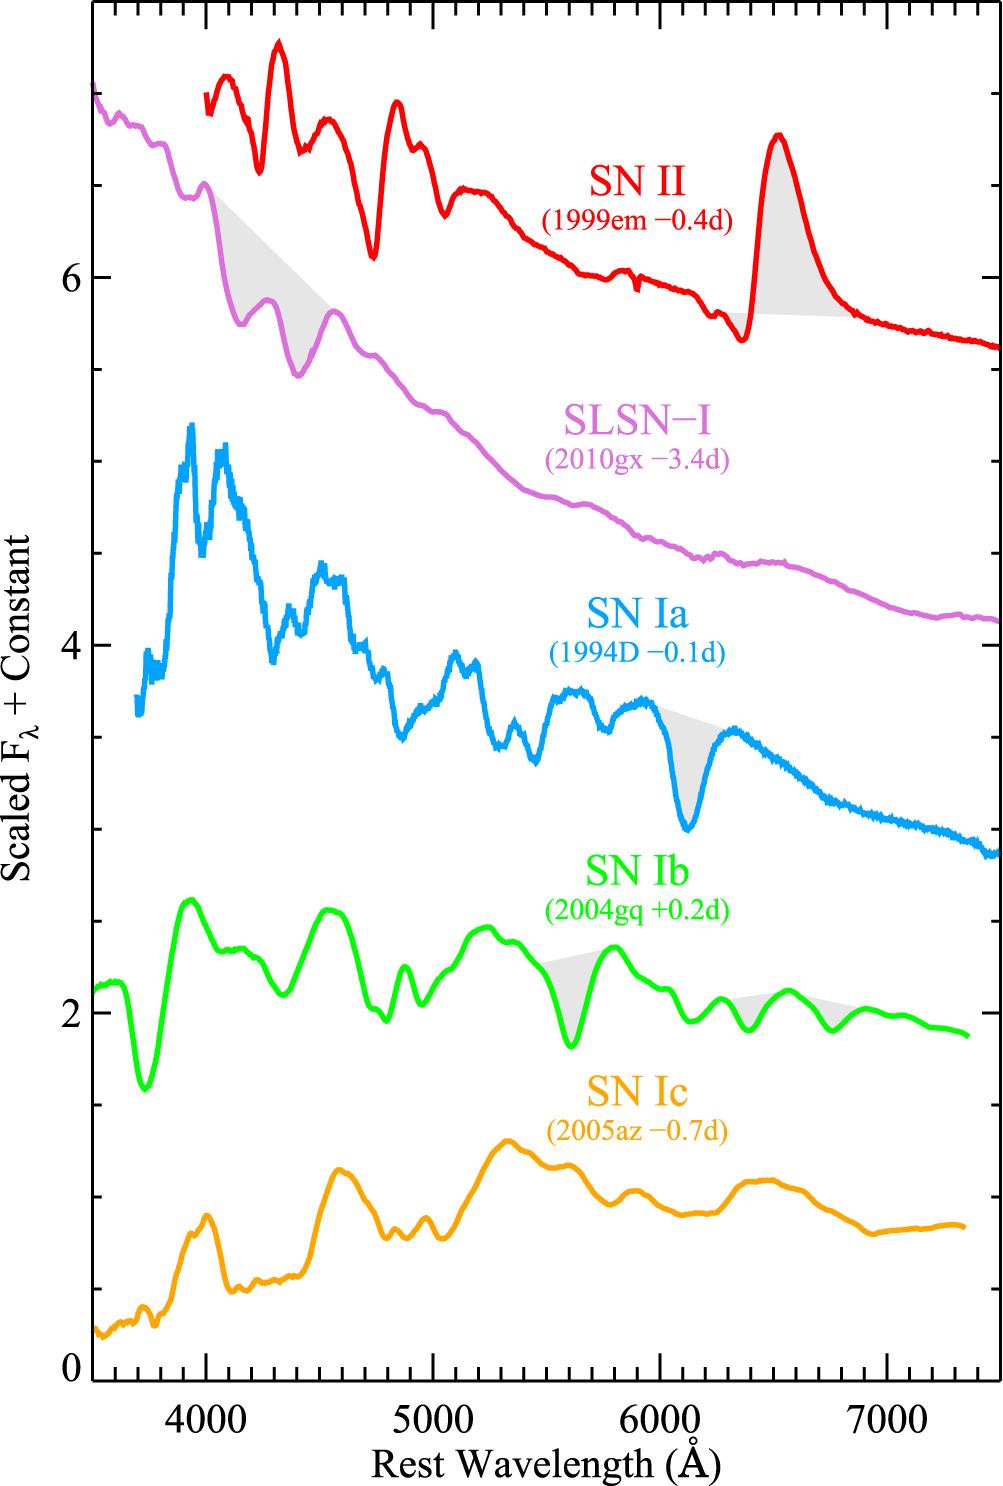
\includegraphics[scale=0.8]{figures/images/supernovae-spectra.jpg}
    \end{minipage}
\end{SCfigure}

\noindent Yet there are small problems that occur here. \\
First, the mechanism which leads to the supernovae explosion is somewhat controversial, since there are two possible scenarios: the ``single-degenerate''-model, in which the companion star is a star of the main sequence or a giant star, and the ``double-degenerate''-model, in which the companion star is also a white dwarf. \\

\noindent In the ``single-degenerate''-model, the accretion must not be too slow, since the hydrogen-rich material of the companion star could be burnt at the same rate as it is accreted, which results in no growth of mass for the white dwarf. On the other hand, the accretion must not be too high, since the accretion might stop due to the companion star's loss of mass at a high rate or being engulfed by the accreted material (\cite[p.~308]{Maguire2017}).

\noindent In the ``double-degenrate''-model, it is assumed that one of both white dwarfs reaches the Chandrasekhar limit if they get too close (\cite[p.~48]{Bartelmann2019}), but there are also other possible scenarios that could occur (see \cite[p.~308/309]{Maguire2017}). \\
\noindent This could lead to slight variations in the luminosity behavior. \\


\noindent Other variations in luminosity behavior could occur due the amount of $^{56}$Ni in the thermonuclear process whose decay influences the peak of the supernovae type Ia light curve (\cite[p.~295]{Maguire2017}). However, those variations can be compensated very well since a relation between the lumninosity's decline and its peak is found so that it is possible to ``normalize'' or ``stretch'' the light curves so they obey a uniform distribution (\cite[p.~4]{Perlmutter2003}, \cite{Phillips1993}).\\
The fact that the light curves of type Ia supernovae are distributed exactly the same way after some ``normalization'' or ``stretching'' shows us that the same physical process underlies all light curves of type Ia supernovae, even if they seem to be stretched, not only due to the relation of luminositys decline and luminositys peak. We will mention later why this property of supernovae type Ia light curves verify the expansion of the universe.

\begin{figure}[H]
    \centering
    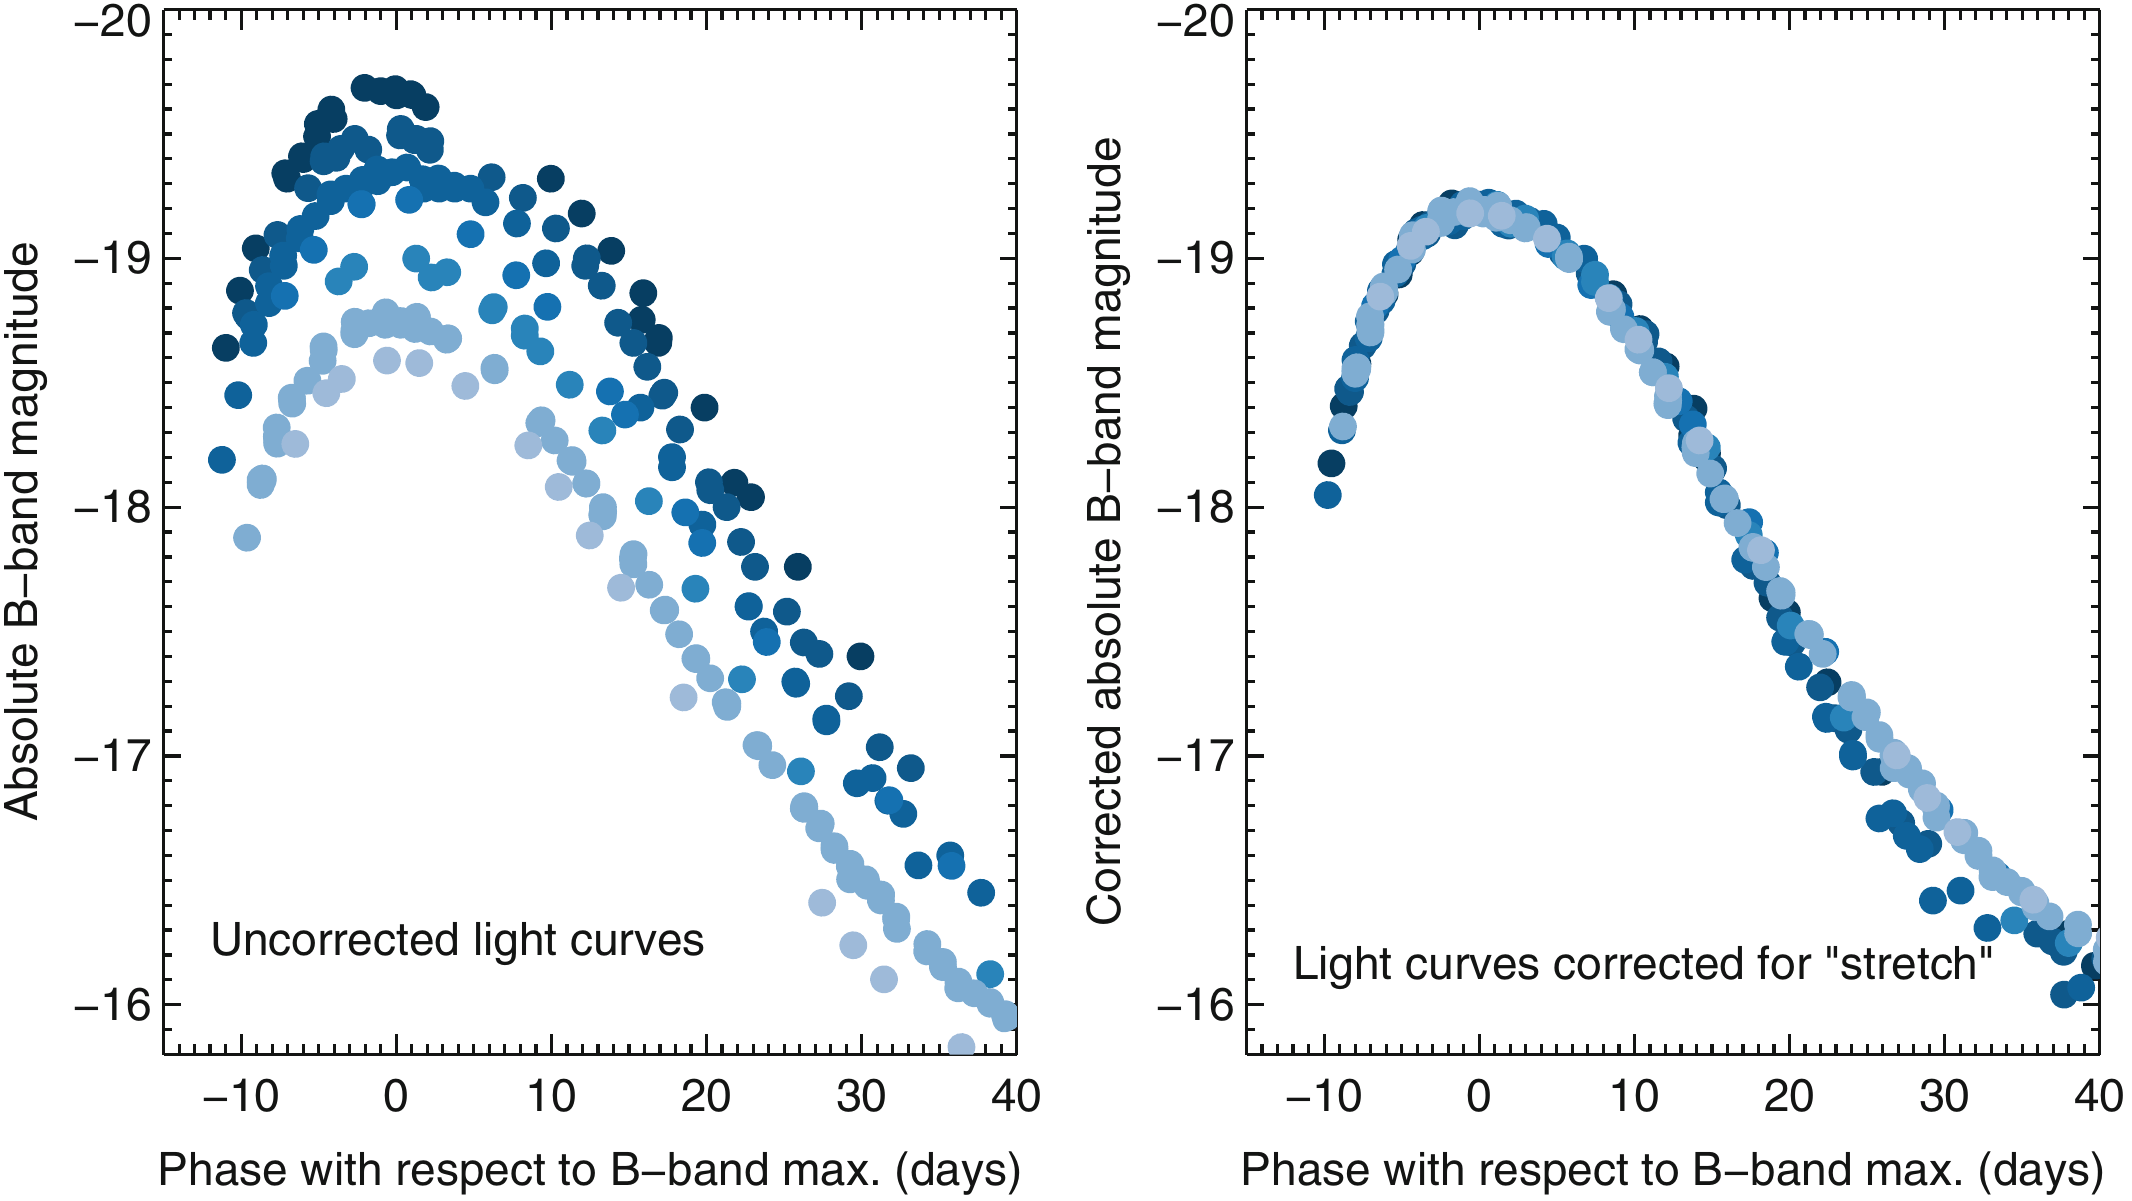
\includegraphics[scale=0.35]{figures/images/supernovae-stretch.png}
    \caption{Uncorrected vs. corrected sample of supernovae type Ia light curves. \\ 
    Source: \cite[p.~298, Figure 2]{Maguire2017}} 
\end{figure}

\noindent Despite the mentioned slight variations in the luminosity spectrum, supernovae of type Ia can be considered as the best candidates for standard candles at the current state of research, not only because their light curves are very homogeneous, but they are also much brighter than cepheids and therefore also visible at large distances, which is essential for cosmological research.


\subsection{Redshift and Hubble's Observation}

The most important tool to determine distances on a cosmological scale is by observing the redshift of extragalactic objects. The redshift is a shift in the observed spectrum of light emmitted by a source with wavelength $\lambda_{\text{e}}$ to an observed wavelength $\lambda_{\text{o}}$ and defined as
\begin{align}
    z := \frac{\lambda_{\text{o}} - \lambda_{\text{e}}}{\lambda_{\text{e}}} = \frac{\lambda_{\text{o}}}{\lambda_{\text{e}}} - 1. \label{eq:redshift}
\end{align}
The term ``red'' in ``redshift'' might be misleading, since $z$ could take also values $<0$ and therefore $\lambda_{\text{o}} < \lambda_{\text{e}}$, which implicates a shift of the light's spectrum to the blue. \\
This term has been established because observations show that the spectrum of most galaxies and extragalactic objects is shifted towards red. \\

\noindent Towards the end of the 1920s, Edwin Hubble observed a certain relation between the measured redshift of the galaxies and extragalactic objects and their distance to us. If one assumes the redshift due to (relativistic) doppler effect,\footnote{Some raised objections against the interpretation that the observed redshift is a result of the doppler effect, but claimed that it is caused by energy loss of the photons traveling through space (``tired light''-hypothesis). We will address later why this hypothesis cannot be hold anymore in the light of tremendous evidence for the expansion model.} one could calculate the galaxies' velocity component towards the direction of observation by
\begin{align}
    z = \gamma \biggl( 1 + \frac{v}{c} \biggr) = \sqrt{\frac{c + v}{c - v}} - 1. \label{eq:relativistic-doppler}
\end{align} 

\noindent An observed shift of the spectrum to the red would imply that the observed object moves away from the observer, and a shift of the spectrum to the blue implies a motion towards the observer. \\
\noindent Edwin Hubble applied a linear relation (see Figure \ref{fig:hubble-law}) between the measured distance $d$ to the observed objects and the calculated velocity $v$ due to the doppler effect
\begin{align}
    v = H_{0} d, \label{eq:hubble-law}
\end{align}
which is known as the \textit{Hubble law}. The proportionality constant $H_{0}$ has the dimension of an inverse time. It is one of the most important parameters in cosmology and its precise determination a challenge of active research (often called ``Hubble tension'', \cite{DiValentino2021}). \\ 

\noindent For small velocities ($v \ll c$), we can approximate Equation \eqref{eq:relativistic-doppler} (first order Taylor series) as $\displaystyle z \approx \frac{v}{c}$, which leads with Equation \eqref{eq:hubble-law} to 
\begin{align}
    d \approx \frac{c}{H_{0}} z. \label{eq:lum-dist-approx} 
\end{align}
We will see later that this relation is actually a first order approximation between the \textit{luminosity distance} $d_{\text{L}}$ and the redshift $z$. \\
The correct relation between the luminosity distance $d_{\text{L}}$ and the redshift $z$ will play an essential role when estimating parameters of cosmological models.

\noindent From Hubble's law follows that the further the distance to a galaxy (or other cosmological object) is, the higher the redshift and therefore, the faster it seems to move apart from us. This observation was one of the milestones in the history of cosmology and was the first indicator that our universe is truly expanding.


\begin{figure}[H]
    \begin{minipage}{8cm}
        \centering 
        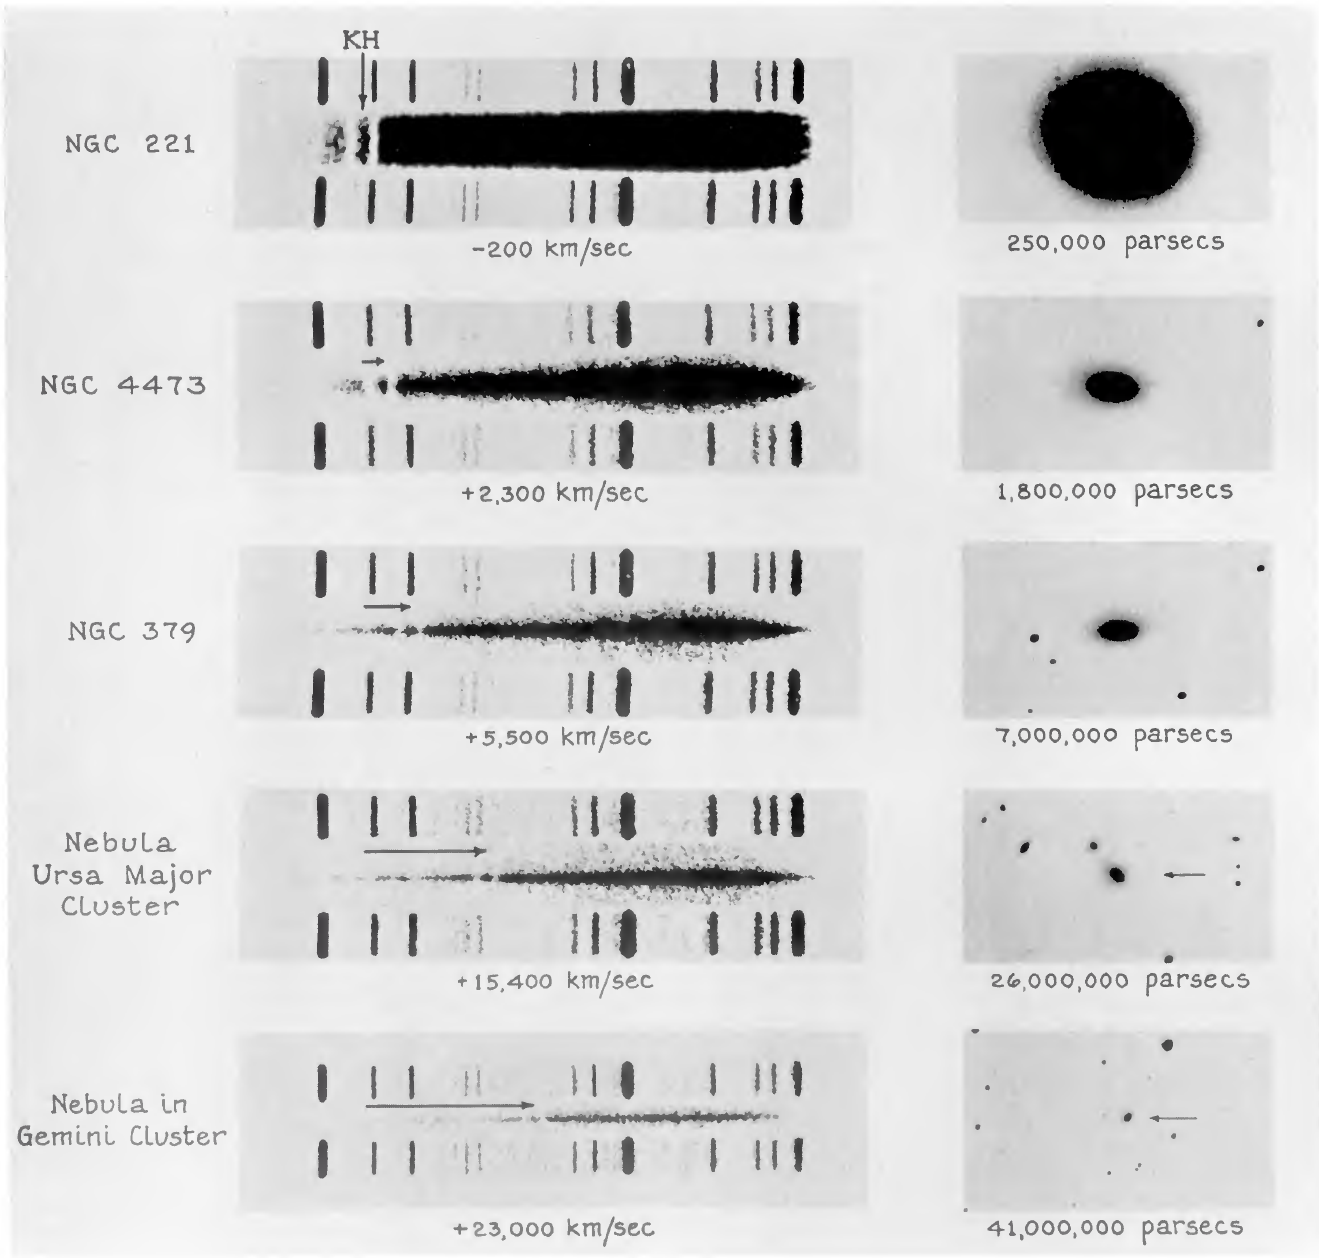
\includegraphics[scale=0.3]{figures/images/humason_redshifts-in-the-spectra-of-extra-galactic-nebulae.png}
        \caption{Observed redshift of H and K lines of calcium, shifted to the red, by Milton L. Humason.  \\ 
        Source: \cite[Figure ``Red-shifts in the Spectra of Extra-galactic Nebulae'']{Humason1936}}
    \end{minipage}
    \hspace{1cm}
    \begin{minipage}{8cm}
        \centering
        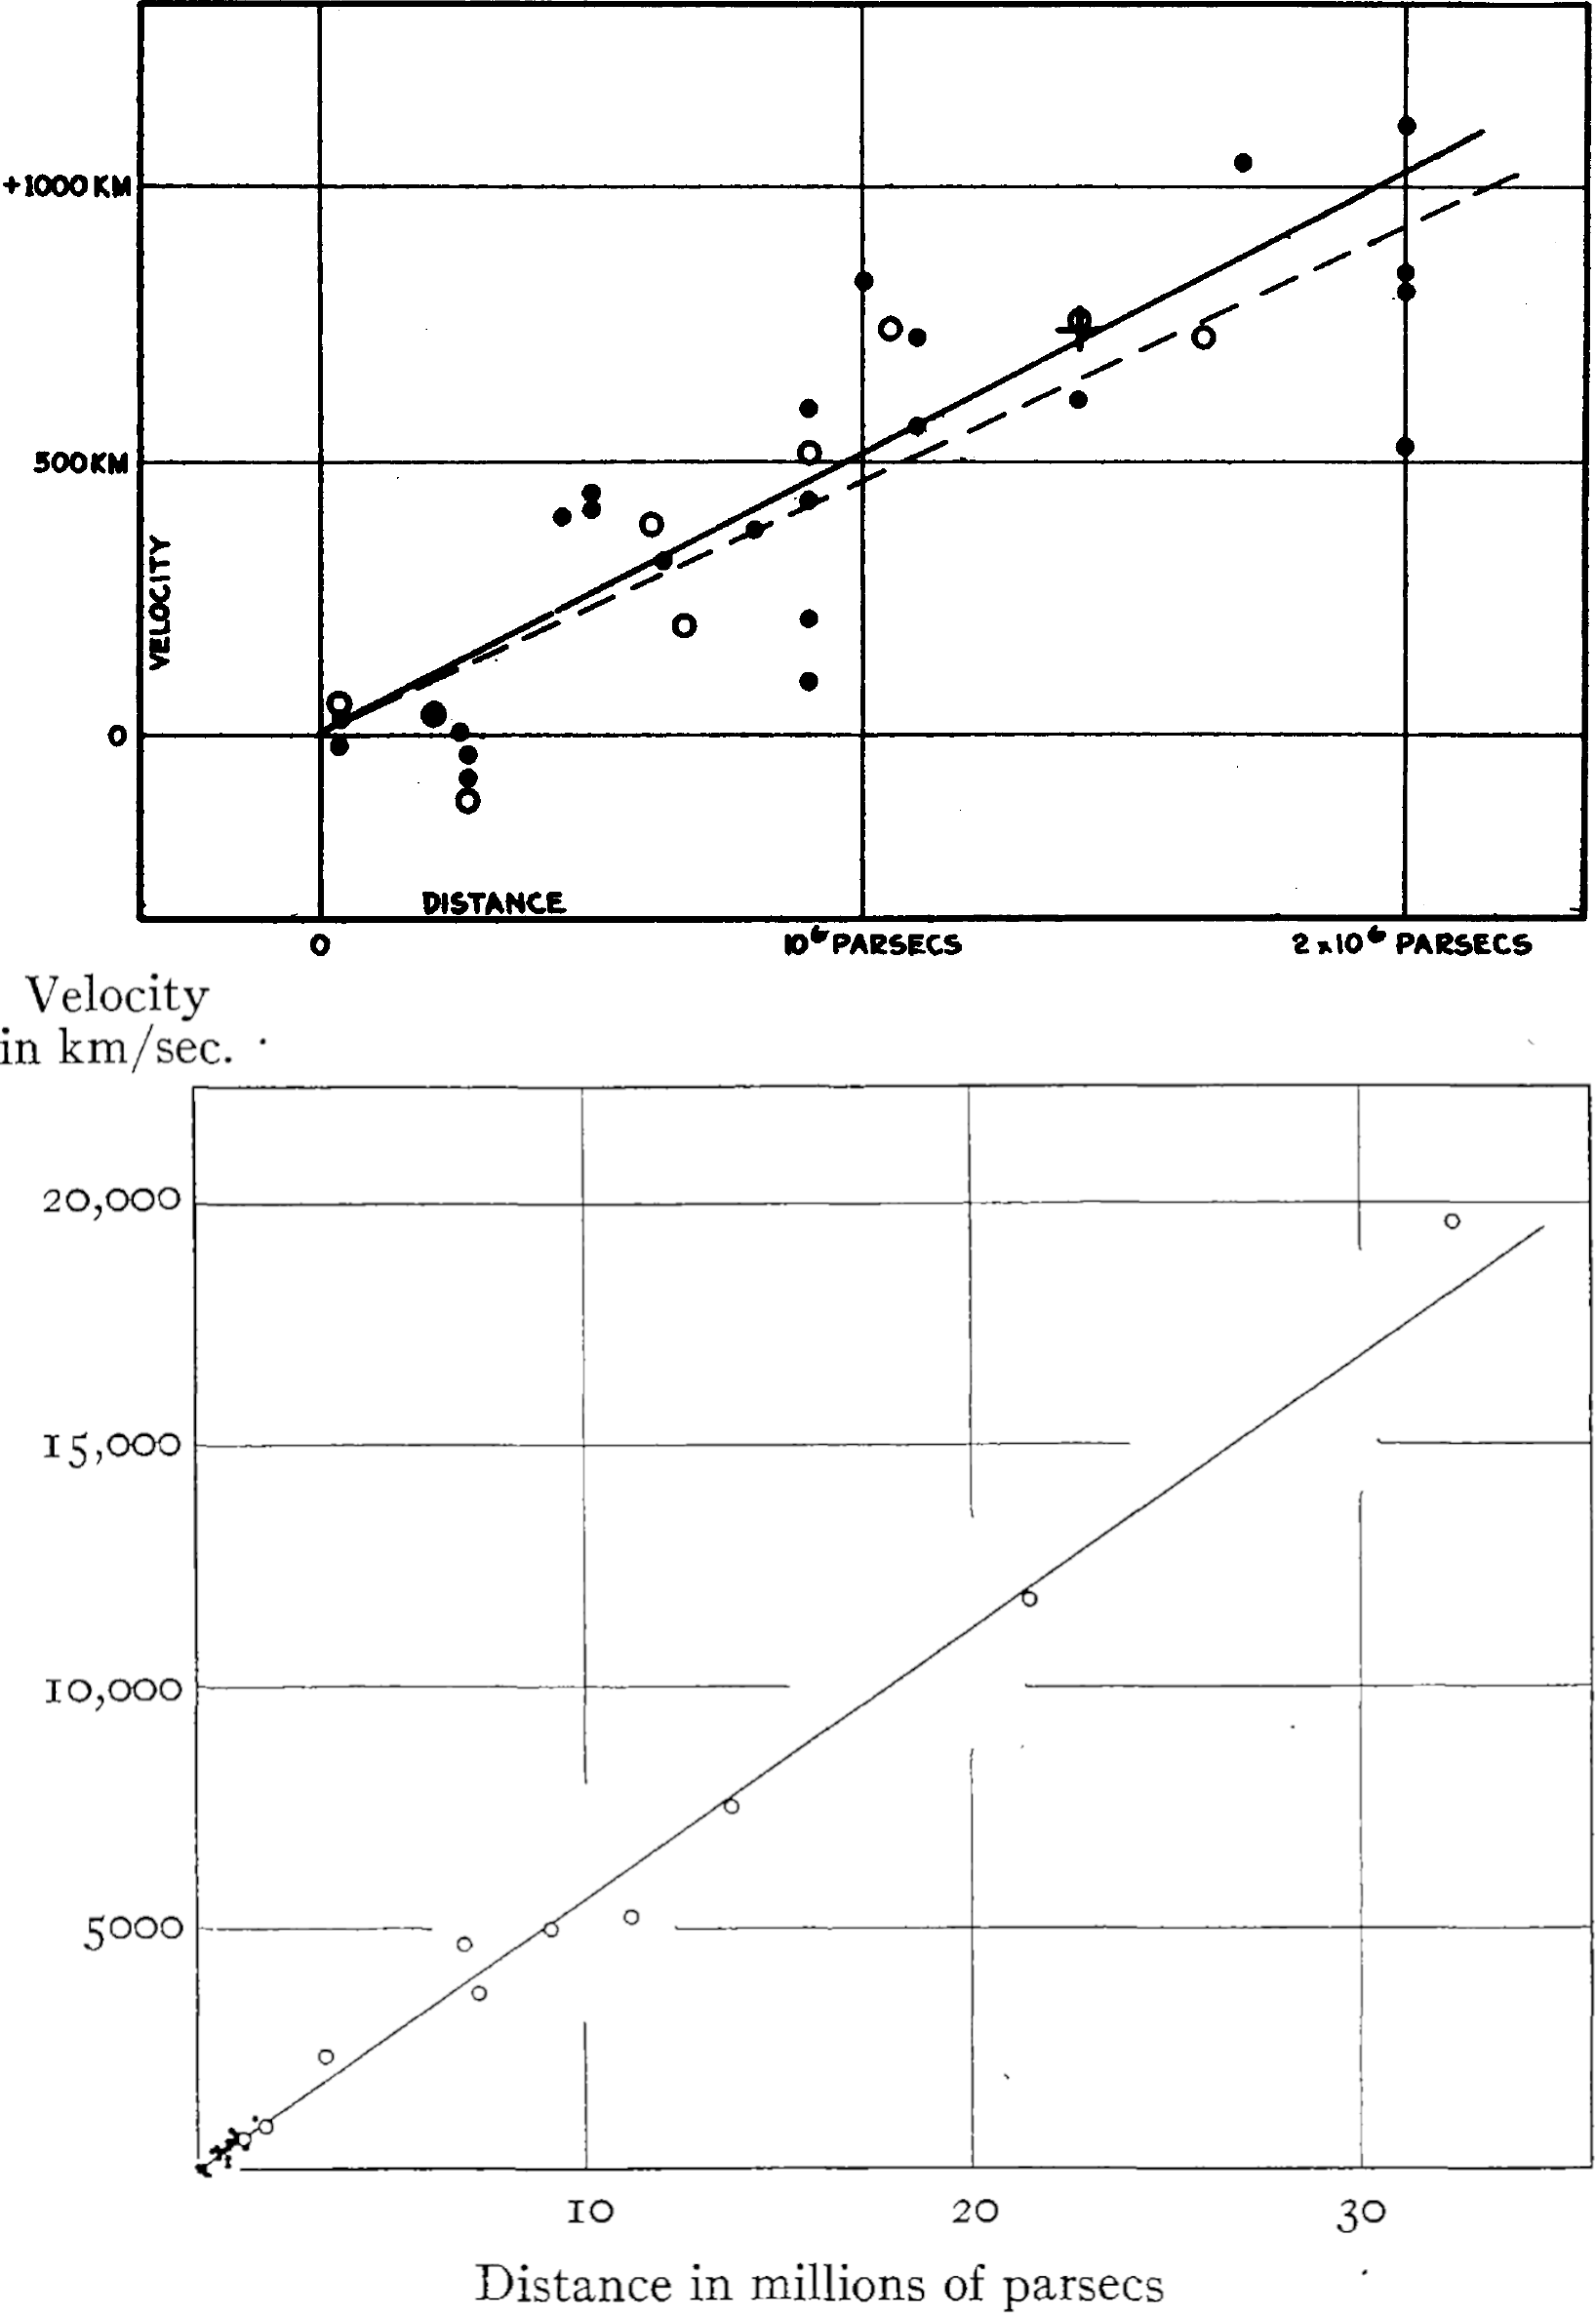
\includegraphics[scale=0.17]{figures/images/hubble_distance-vs-velocity.png}
        \caption{Linear regression between the distance of observed objects and the calculated velocity due to redshift. \\ 
        Source: \cite{Hubble1929} and \cite[Figure 5]{Hubble1931}}
        \label{fig:hubble-law}
    \end{minipage}    
\end{figure}



\section{The Theory of Gravity and Spacetime}
How can one speak about the nature on large scales without mentioning the force that dominates in this regime?
Beginning with Newton's ideas about gravity, the modern formulation about gravity is described in the framework of Einstein's general theory of relativity, in which gravity is, strictly speaking, not anymore a force in the Newtonian sense, but rather a property of the four dimensional spacetime that interacts with matter. \\

\noindent For a deep understanding of general relativity, it is required to have knowledge on the mathematics of differential geometry. \\
\noindent Besides the fact that, as an undergraduate student, I do not (yet) possess this knowledge, this would be beyond the scope of this bachelor thesis. \\
\noindent However, to motivate the basic equations of the $\Lambda$CDM-model, which are derived from Einstein's field equations under certain assumptions that we are going to formulate in the next chapter, I would like to mention the concept of a \textit{metric} and give brief view on Einstein's field equations.

\subsection{The Metric of Spacetime}
Generally speaking, a metric is a function that takes two points in space and returns a distance. \\
For example, let $\mathbb{E}^2$ be the Euclidean, two dimensional space, then
\begin{align}
    d(\cdot, \cdot) : \mathbb{E}^{2} \times \mathbb{E}^{2} \to \R, (\vb*{p}_{1}, \vb*{p}_{2}) \mapsto d(\vb*{p}_{1}, \vb*{p}_{2}) := \sqrt{(x_{1} - x_{2})^2 + (y_{1} - y_{2})^2} 
\end{align}
would be a function that gives us the distance between two points $\vb*{p}_{1} = (x_{1}, y_{1})^{\intercal}$ and $\vb*{p}_{2} = (x_{2}, y_{2})^{\intercal}$. This distance function $d$ would return the Pythagorean distance in Cartesian coordinates that we are familiar with. \\
Let us define $x := x_{1} - x_{2}$, $y := y_{1} - y_{2}$ and $s := d(\vb*{p}_{1}, \vb*{p}_{2})$ so we could write for the (infinitesimal) distance 
\begin{align}
    \dd{s}^2 = \dd{x}^2 + \dd{y}^2. \label{eq:line-element-cartesian}
\end{align}
Now, let us switch to polar coordinates so that $\vb*{p}_{1} := (r_{1}, \phi_{1})^{\intercal}$ and $\vb*{p}_{2} := (r_{2}, \phi_{2})^{\intercal}$. With the given distance function $d$, we would obtain 
\begin{align}
    d(\vb*{p}_{1}, \vb*{p}_{2}) = \sqrt{(r_{1} - r_{2})^2 + (\phi_{1} - \phi_{2})^2}, 
\end{align}
but this is \textit{not} the same distance as in Cartesian coordinates. The distance that would correspond to the same distance as in Cartesian coordinates (see Equation \eqref{eq:line-element-cartesian}), is
\begin{align}
    \dd{s}^2 = \dd{r}^2 + r^2 \dd{\phi}^2 
\end{align}
with $r:= r_{1} - r_{2}$, $\phi := \phi_{1} - \phi_{2}$. \\
\noindent We have to introduce the \textit{metric tensor} (in most applications of physics a $3 \times 3$- or $4 \times 4$-matrix) that guarantees the invariance of the distance function $d$ under coordinate transformation. \\
We define 
% \begin{align}
%     \begin{pmatrix} 1 && 0 \\ 0 && 1 \end{pmatrix} \overset{\text{cartesian}}{=} g_{ij} \overset{\text{polar}}{=} \begin{pmatrix} 1 && 0 \\ 0 && r \end{pmatrix}, \quad x \overset{\text{cartesian}}{=} x^{1} \overset{\text{polar}}{=} r, \quad y \overset{\text{cartesian}}{=} x^{2} \overset{\text{polar}}{=} \phi, 
% \end{align}
\begin{align}
    g_{ij} := \begin{cases} \begin{pmatrix} 1 && 0 \\ 0 && 1 \end{pmatrix} \quad \text{in cart.} \\  \begin{pmatrix} 1 && 0 \\ 0 && r \end{pmatrix} \quad \text{in polar} \end{cases} x^{1} := \begin{cases} x \quad \text{in cart.} \\ r \quad \text{in polar} \end{cases}  x^{2} := \begin{cases} y \quad \text{in cart.} \\ \phi \quad \text{in polar} \end{cases}
\end{align}
% \begin{align}
%     g_{ij} &\overset{\text{cartestian}}{=} \begin{pmatrix} 1 && 0 \\ 0 && 1 \end{pmatrix} \overset{\text{polar}}{=} \begin{pmatrix} 1 && 0 \\ 0 && r \end{pmatrix}, \quad x^{1} = \begin{cases} x \quad \text{cartestian} \\ r \quad \text{polar}\end{cases},  \quad x^{2} = \begin{cases} y \quad \text{cartesian} \\ \phi \quad \text{polar} \end{cases}
% \end{align}
so that we can express the invariant distance between $\vb*{p}_{1}$ and $\vb*{p}_{2}$ through
\begin{align}
    \dd{s}^2 &= \sum_{i = 1}^{2} \sum_{j = 1}^{2} g_{ij}\dd{x}^{i}\dd{x}^{j} = g_{11} \bigl(\dd{x}^{1}\bigr)^2 + \underbrace{g_{12}}_{= 0} \dd{x}^{1}\dd{x}^{2} + \underbrace{g_{21}}_{= 0} \dd{x}^{2} \dd{x}^{1} + g_{22} \bigl(\dd{x}^{2} \bigr)^2 \\
             &= g_{11} \bigl(\dd{x}^{1}\bigr)^2 + g_{22} \bigl(\dd{x}^{2}\bigr)^2 \overset{\text{cart.}}{=} \dd{x}^{2} + \dd{y}^{2} \overset{\text{polar}}{=} \dd{r}^{2} + r^2 \dd{\phi}^{2}.  
\end{align}

\noindent In the framework of relativity, we express the distance (called ``world line'') between to \textit{events} $\vb*{p}_{1} := (c t_{1}, x_{1}, y_{1}, z_{1})^{\intercal}$ and $\vb*{p}_{2} := (c t_{2}, x_{2}, y_{2}, z_{2})^{\intercal}$ in four dimensional spacetime as
\begin{align}
    \dd{s}^2 = g_{\mu\nu} \dd{x}^{\mu} \dd{x}^{\nu}
\end{align}
with the implicit sum over double occuring indices $\mu, \nu \in \{0,1,2,3\}$. In flat Minkowski-spacetime of special relativity for example, we have 
\begin{align}
    g_{\mu\nu} = \eta_{\mu\nu} := \diag(-1, 1, 1, 1) 
\end{align} 
and therefore for distances in spacetime
\begin{align}
    \dd{s}^2 = \eta_{\mu\nu} \dd{x}^{\mu} \dd{x}^{\nu} = - (c \dd{t})^{2} + \dd{x}^{2} + \dd{y}^{2} + \dd{z}^{2}.    
\end{align}



\subsection{Einstein's Field Equations}

\noindent Similar to the derivation of the Euler--Lagrange equations in classical mechanics (or classical field theory) by formulating an action $S[\vb*{q}(t)]$ (or $S[\phi(x)]$) and find the path $\vb*{q}(t)$ (or field $\phi(x)$) that extremizes the action ($\delta S = 0$), Einstein's field equations can be derived\footnote{For a proper and detailed derivation, see subsection 4.3 ``\textit{Lagrangian Formulation}'' in \cite[p.~159]{SeanCarroll2019}.} from the Einstein--Hilbert action given by
\begin{align}
    S_{\text{EH}}[g_{\mu\nu}] = \int \dd[4]{x} \sqrt{-\det(g_{\mu\nu})} \biggl[\frac{c^4}{16\pi G}(R - 2\Lambda) + \mathcal{L}_{\text{M}} \biggr], 
\end{align}
where $\dd[4]{x}$ is the four dimensional spacetime-volume element, $g_{\mu\nu}$ the metric tensor, $c$ the speed of light (in vacuum), $G$ the Newtonian gravitational constant, $R$ the Ricci scalar, $\Lambda$ the cosmological constant, and $\mathcal{L}_{\text{M}}$ the Lagrange density of matter fields. 

\noindent With the action principle, the variation $\delta S[g_{\mu\nu}]$ of the Einstein--Hilbert action with respect to the metric leads to Einstein's field equations
\begin{align}
    R_{\mu\nu} - \frac{1}{2}R g_{\mu\nu} + \Lambda g_{\mu\nu} = \frac{8\pi G}{c^4}T_{\mu \nu}, \label{eq:einstein-field-equations}
\end{align}
where $R_{\mu\nu}$ is the Ricci curvature tensor and $T_{\mu\nu}$ the energy-momentum tensor. \\
\noindent Without getting too much into details about the single components of this equation, we keep in mind that the left-hand side of Equation \eqref{eq:einstein-field-equations} describes how spacetime behaves, while the right-hand side of Equation \eqref{eq:einstein-field-equations} describes how matter behaves.

\subsubsection{The Cosmological Constant $\Lambda$}

\noindent Originally, Einstein formulated his field equations without the cosmological constant $\Lambda$. Since Einstein believed in a static universe and found that his equations cannot hold for a static universe (it would have collapsed due to the gravity of matter), he introduced the $\Lambda$ term that acts repulsive towards the attraction of gravity, so that a static universe as he proposed would be possible. \\



%%% THE STANDARD MODEL OF COSMOLOGY
\chapter{The Standard Model of Cosmology}
\thispagestyle{empty}

\bt

\section{The Cosmological Principle}

\subsection{Homogenity}

\subsection{Isotropy}

\section{Friedmann equations}

\subsection{FLRW-Metric}

\subsection{Cosmological Parameters}

\section{Evidence}


%%% THE DVALI-GABADADZE-PORRATI MODEL
\chapter{The Dvali--Gabadadze--Porrati-Model}
\label{chap:the-dvali-gabadadze-porrati-model}
\thispagestyle{empty}

The model proposed by Gia Dvali, Gregory Gabadadze and Massimo Porrati (\cite{Dvali2000}) is an alternative cosmological model, in which our four-dimensional universe is embedded as a brane in a five-dimensional Minkowski spacetime. \\
The authors introduce a fourth spatial dimension $y$. While the electromagnetic, the weak and the strong nuclear force are limited to our four-dimensional world, gravity also acts onto the postulated additional spatial dimension. \\
The scale to which gravity acts familiar as the theory of general relativity predicts, but mimics dark energy as it acts onto the additional dimension, is introduced as the crossover scale $r_{\text{c}}$. \\
From the modified Einstein--Hilbert-action given by (see \cite{Dvali2003}) 
\begin{align}
    S_{\text{DGP}} = \frac{1}{r_{\text{c}}} \frac{c^4}{8\pi G} \int \dd[4]{x} \dd{y} \sqrt{-\det(g_{AB}^{(5)})} \mathcal{R} + \int \dd[4]{x} \sqrt{-\det(g_{\mu \nu})} \biggl(\frac{c^4}{8 \pi G} R + \mathcal{L}_{\text{SM}} \biggr),
\end{align}
where $g_{AB}^{(5)}$ is the metric with $A, B \in \{0, 1, 2, 3, 4\}$ and $\mathcal{R}$ the Ricci scalar on five-dimensional spacetime, follow the modified Einstein field equations 
\begin{align}
    \frac{1}{r_{\text{c}}} \mathcal{G}_{AB} + \delta(y) \delta_{A}^{\mu} \delta_{B}^{\nu} \biggl( G_{\mu \nu} - \frac{8\pi G}{c^4} T_{\mu \nu} \biggr) = 0, 
\end{align}
where $G_{\mu \nu} = R_{\mu \nu} - \frac{1}{2} R g_{\mu \nu}$ is the Einstein tensor (left-hand-side of Equation \eqref{eq:einstein-field-equations} without cosmological constant $\Lambda$) and $\mathcal{G}_{AB}$ its five-dimensional analogon. An ansatz as proposed in \cite{Dvali2003}, the metric 
\begin{align}
    \dd{s}_{(5)}^2 = f(y,H) \dd{s}^2 - \dd{y}^2, 
\end{align}
where $\dd{s}^2$ is the four-dimensional maximally-symmetric FLRW-metric, $H$ the four-dimensional Hubble parameter and $f(y, H)$ the so called warp-factor, leads to the modified Friedmann equation
\begin{align}
    H^{2} \pm \frac{c}{r_{\text{c}}}H = \frac{8 \pi G}{3} \rho.  \label{eq:modified-friedmann1}
\end{align}
The positive sign accounts to a decelerated expansion, while a negative sign corresponds to an accelerated expansion. Thus, we consider in the following the case in which the sign in Equation \eqref{eq:modified-friedmann1} is negative. \\

\noindent We are now introducing the parameter $\alpha \in \R$ which should interpolate between the $\Lambda$CDM-model in the case of neglecting radiation in a flat universe ($\Omega_{\text{r},0} = 0, \Omega_{k,0} = 0$) for $\alpha = 0$ and the DGP-model for $\alpha = 1$. Therefore, we can rewrite Equation \eqref{eq:modified-friedmann1} in the accelerated case as 
\begin{align}
    H^{2} - \biggl(\frac{c}{r_{\text{c}}} \biggr)^{2 - \alpha} H^{\alpha} = \frac{8 \pi G}{3} \rho
\end{align}
and can conclude with Equation \eqref{eq:critical-density}, Equation \eqref{eq:matter-density-scale}, and the crossover scale expressed by (\cite[p.~3]{Dvali2003})
\begin{align}
    r_{\text{c}} = \frac{c}{H_{0}}(1 - \Omega_{\text{m},0})^{\frac{1}{\alpha - 2}}, 
\end{align}
the equation 
\begin{align}
    E^{2}(z) - (1 - \Omega_{\text{m},0}) E^{\alpha}(z) - \Omega_{\text{m},0} (1 + z)^3 = 0, \label{eq:dgp-friedmann-interpolation} 
\end{align}
where $\displaystyle E(z) = \frac{H(z)}{H_{0}}$ is the expansion function. \\

\noindent The DGP-model refrains from introducing a cosmological constant. The free parameters of the DGP-model are therefore $\Omega_{\text{m},0}$ and $\alpha$.
We consider in this thesis the DGP-model of a flat universe. The definition of the luminosity distance $d_{\text{L}}$ remains the same as in the $\Lambda$CDM-model (see Equation \eqref{eq:luminosity-distance}). \\
Since a deeper understanding of the mathematical formalism of the DGP-model and a detailed description of its phenomenological implications would go beyond the scope of this thesis, I recommend for further readings \cite{Lue2006}.


%%% PARAMETER ESTIMATION
\chapter{Parameter Estimation}
\label{chap:parameter-estimation}
\thispagestyle{empty}

Let us now compare the $\Lambda$CDM- and DGP-model. To do this, we will consider the ``Union2.1'' SN Ia compilation and determine best-fit values for the parameter pair ($\Omega_{\text{m},0}$, $\Omega_{\Lambda,0}$) in $\Lambda$CDM- and ($\Omega_{\text{m},0}$, $\alpha$) in DGP-model by computing the $\chi^2$-distribution, which is a measure for the likelihood.

\section{Supernovae Type Ia ``Union2.1'' Dataset}

\noindent The SN Ia ``Union2.1'' dataset (see appendix \ref{app:dataset-and-source-codes}) used in this thesis contains the name, the redshift, the distance modulus, and the distance modulus error of 580 supernovae, measured by the Hubble Space Telescope. \\

\noindent First, let us have a look at the dataset. We plot the distance modulus (see Equation \eqref{eq:distance-modulus}) $m - M$ against the redshift $z$ for the predicted luminosity distance $d_{\text{L}}$ by the $\Lambda$CDM-model with $(\Omega_{\text{m},0}, \Omega_{\Lambda,0}) = (0.3, 0.7)$ and DGP-model with $(\Omega_{\text{m}}, \alpha)=(0.3, 1.0)$.

\begin{figure}[H]
   \centering
   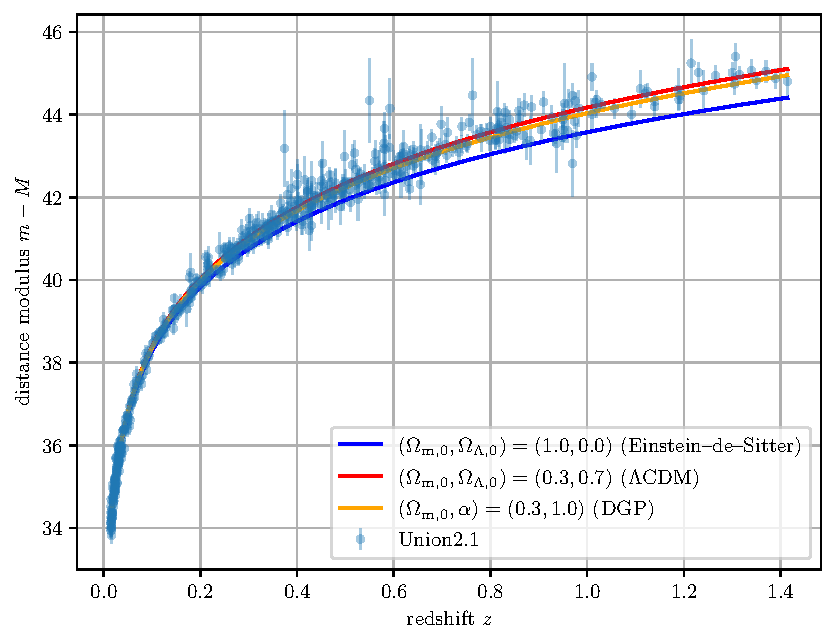
\includegraphics[scale=0.97]{figures/plots/PDF/redshift-vs-distance-modulus.pdf}
   \caption{Distance modulus $m - M$ against redshift $z$ for Einstein--de--Sitter-model $(\Omega_{\text{m},0}, \Omega_{\Lambda,0}) = (1.0, 0.0)$, the $\Lambda$CDM-model with $(\Omega_{\text{m},0}, \Omega_{\Lambda,0}) = (0.3, 0.7)$ and DGP-model with $(\Omega_{\text{m},0}, \alpha) = (0.3, 1.0)$.\\}
   \label{fig:redshift-vs-distance-modulus}
\end{figure}

\noindent At first sight, we see that a universe that contains only matter (Einstein--de--Sitter-model) cannot match the data, especially for high redshifts. \\
Further, we can conclude that the data points at high redshift ($z \gtrsim 0.8$) have a greater influence on the fit for the estimated parameters, since there is no significant fluctuation of data points at low redshift. \\
The apparently large errors of some data points in the range of $0.35 \leq z \leq 1.0$ should not cause any concerns whether this dataset is suitable for an adequate parameter estimation, since the error of low-redshift data points will impact the fit to a lesser degree than errors in high-redshift data points.

\section{Statistical Analysis}
To obtain values for the best-fit parameters, we consider the distance of every data point between its \textit{measured} relative magnitude to the \textit{theoretical} value the relative magnitude would have dependent on the parameters of the model. \\ 
From now on, we denote $\vb*{\theta}$ as the parameter pairs of the model we want to estimate, so 
\begin{align}
    \vb*{\theta} = \begin{cases}
                        (\Omega_{\text{m},0}, \Omega_{\Lambda,0}) &\text{for $\Lambda$CDM-model}\\
                        (\Omega_{\text{m},0}, \alpha)             &\text{for DGP-model}\\
                   \end{cases}. \label{eq:cosmological-parameters}
\end{align}
The given dataset is a sample of $N = 580$ datapoints which contain for datapoint $i \in [1,N]$ the redshift $z_{i}$, the distance modulus and therefore implicitly\footnote{Although the ``Union2.1'' SN Ia compilation contains the distance modulus $m - M$, we will handle it throughout the parameter estimation as if it only contains the relative magnitude $m$. Since we are going to marginalize the parameter $M$, it has no influence on the parameter estimation.} the relative magnitude $m_{i}$ and its error $\sigma_{m_{i}}$. \\
Our goal is to express the quantities given \textit{only} through the free parameters $\vb*{\theta}$. \\
Now, let us consider the relative magnitude $m$, which is given by the distance modulus (see Equation \eqref{eq:distance-modulus}). First, we want to express the luminosity distance $d_{\text{L}}$ in multiples of $\SI{1}{\mega \parsec}$, so we obtain
\begin{align*}
    m &= M + 5\log_{10}\biggl( \frac{d_{\text{L}}}{\SI{10}{\parsec}} \biggr) = M + 5\log_{10}\biggl( 10^{5} \frac{d_{\text{L}}}{\SI{1}{\mega \parsec}} \biggr) \\
      &= M + 25 + 5\log_{10}\biggl(\frac{d_{\text{L}}}{\SI{1}{\mega \parsec}}\biggr). 
\end{align*}
Since the luminosity distance $d_{\text{L}}$ depends on the Hubble distance $d_{\text{H}}$ (see Equation \eqref{eq:comoving-distance} and \eqref{eq:luminosity-distance}) and is therefore proportional to $d_{\text{L}} \propto 1/H_{0}$, we redefine the luminosity distance so that it is independent of the Hubble constant. Hence, we go on with 
\begin{align}
m &= M + 25 + 5\log_{10} \biggl(\frac{1}{H_{0}} H_{0} d_{\text{L}}(z, H_{0}, \vb*{\theta}) \SI{}{\mega \parsec^{-1}} \biggr) \nonumber \\
  &= \underbrace{M + 25 - 5\log_{10}(H_{0})}_{ =: \mathcal{M}(H_{0}) } + 5 \log_{10} \biggl( \underbrace{H_{0} d_{\text{L}}(z, H_{0}, \vb*{\theta})}_{ =: \mathcal{D}_{\text{L}}(z, \vb*{\theta}) } \SI{}{\mega \parsec^{-1}} \biggr) \nonumber \\
  &= \mathcal{M}(H_{0}) + 5 \log_{10}(\mathcal{D}_{\text{L}}(z, \vb*{\theta}) \SI{}{\mega \parsec^{-1}}). \label{eq:relative-magnitude_mod-magnitude_mod-luminosity-distance}
\end{align}
With Equation \eqref{eq:relative-magnitude_mod-magnitude_mod-luminosity-distance}, the dependency on the Hubble constant is now in an additive constant $\mathcal{M}(H_{0})$, which will be useful as we see later. \\

\noindent From now on, we are going to call the relative magnitude in Equation \eqref{eq:relative-magnitude_mod-magnitude_mod-luminosity-distance} the \textit{theoretical} relative magnitude $m_{\text{th}}$, since it contains the cosmological parameters $\vb*{\theta}$. \\ 

\noindent Given the dataset $D := \{z_{i}, m_{i}, \sigma_{m_{i}} \}$, where $z_{i}$ is the measured redshift, $m_{i}$ the measured relative magnitude and $\sigma_{m_{i}}$ the error of the relative magnitude $m_{i}$, we define 

\begin{align}
    \chi^2(\mathcal{M}, \vb*{\theta} \vert D) := \sum_{i=1}^{N} \biggl(\frac{m_{\text{th}}(z_{i}, \mathcal{M}, \vb*{\theta}) - m_{i}}{\sigma_{m_{i}}}\biggr)^2 \label{eq:chi-square} 
\end{align}
as the $\chi^2$-distribution of $\mathcal{M}$ and $\vb*{\theta}$. \\
\noindent The likelihood, which is a probability density, is given by 
\begin{align}
    L(\mathcal{M}, \vb*{\theta} \vert D) := L_{0} \exp \biggl(-\frac{1}{2} \chi^2(\mathcal{M}, \vb*{\theta} \vert D) \biggr),  \label{eq:likelihood}
\end{align}
where $L_{0}$ is a normalization factor.
With the likelihood $L$, it is possible to calculate the probability $P$ to find $\mathcal{M} \in \mathcal{I}_{\mathcal{M}}$ and $\vb*{\theta} \in \mathcal{I}_{\vb*{\theta}}$ in a parameter interval $\mathcal{I}_{\mathcal{M}}$ and $\mathcal{I}_{\vb*{\theta}}$ with 

\begin{align}
    P(\mathcal{M} \in \mathcal{I}_{\mathcal{M}}, \vb*{\theta} \in \mathcal{I}_{\vb*{\theta}} \vert D) = \int\limits_{\mathcal{I}_{\mathcal{M}}} \dd{\mathcal{M}} \int\limits_{\mathcal{I}_{\vb*\theta}} \dd{\vb*{\theta}} L(\mathcal{M}, \vb*{\theta} \vert D). \label{eq:probability}   
\end{align}
However, this probability $P$ still depends on $\mathcal{M}$, which is not measured. Since our goal is to find the best-fit values for $\vb*{\theta}$ and therefore express the probability only through $\vb*{\theta}$, we are going to \textit{marginalize} over $\mathcal{M}$. We obtain the \textit{marginalized} likelihood $L_{\text{M}}$ by integrating the likelihood $L$ over all possible values that $\mathcal{M}$ could take. Assuming $\mathcal{M} \in (-\infty, \infty)$, it follows  
\begin{align}
    L_{\text{M}}(\vb*{\theta} \vert D) = \int\limits_{-\infty}^{\infty} \dd{\mathcal{M}} L(\mathcal{M}, \vb*{\theta} \vert D). \label{eq:marginalized-likelihood} 
\end{align}
Thereby, we can calculate the probability $P(\vb*{\theta} \in \mathcal{I}_{\vb*{\theta}} \vert D)$ to find values for $\vb*{\theta} \in \mathcal{I}_{\vb*{\theta}}$, given the dataset $D$, but without any information on $\mathcal{M}$, which implicitly contains the Hubble constant $H_{0}$, so
\begin{align}
    P(\vb*{\theta} \in \mathcal{I}_{\vb*{\theta}} \vert D) = \int\limits_{\mathcal{I}_{\vb*{\theta}}} \dd{\vb*{\theta}} L_{\text{M}}(\vb*{\theta} \vert D). \label{eq:marginalized-probability}
\end{align}
Since $\mathcal{M}$ is only an additive constant (see Equation \eqref{eq:relative-magnitude_mod-magnitude_mod-luminosity-distance}), this can be done analytically. To do so, we set $\mathcal{M} = 0$ and introduce the terms
\begin{align}
    c_{1}(\{\sigma_{m_{i}} \}) &:= \sum_{i = 1}^{N} \frac{1}{\sigma_{m_{i}}^2}, \\
    b_{0}(\vb*{\theta} \vert D) &:= \sum_{i = 1}^{N} \frac{m_{\text{th}}(z_{i}, \vb*{\theta}) - m_{i}}{\sigma_{m_{i}}^2}, \\
    b_{1}(\vb*{\theta} \vert D) &:= \sum_{i = 1}^{N} \biggr(\frac{m_{\text{th}}(z_{i}, \vb*{\theta}) - m_{i}}{\sigma_{m_{i}}} \biggl)^2,
\end{align}
by which we obtain
\begin{align}
    \chi^2 (0, \vb*{\theta} \vert D) = b_{1}(\vb*{\theta} \vert D) - \frac{b_{0}^2 (\vb*{\theta} \vert D)}{c_{1}(\{ \sigma_{m_{i}} \})} =: \chi_{\text{A}}^2 (\vb*{\theta} \vert D) \label{eq:analytic-chi-square} 
\end{align}
and thus for the likelihood
\begin{align}
    L(0, \vb*{\theta} \vert D) = L_{0} \exp \biggl(-\frac{1}{2} \chi_{\text{A}}^2(\vb*{\theta} \vert D) \biggr) =: L_{\text{A}}(\vb*{\theta} \vert D). \label{eq:analytic-likelihood} 
\end{align}
The expressions $L_{\text{M}}$ (see Equation \eqref{eq:marginalized-likelihood}) and $L_{\text{A}}$ (see Equation \eqref{eq:analytic-likelihood}) lead to the same results, which we will check later for a minimal working example in the case of the $\Lambda$CDM-model. In the following, we denote the likelihood and the $\chi^2$-distribution that are independent of $\mathcal{M}$ simply as $L(\vb*{\theta} \vert D)$ and $\chi^2(\vb*{\theta} \vert D)$. 

\noindent The best-fit parameters $\vb*{\theta}_{\text{best}}$ are located at the maximum of the likelihood, so 
\begin{align}
    \pdv{L(\vb*{\theta} \vert D)}{\vb*{\theta}} \bigg \vert_{\vb*{\theta}_{\text{best}}} = 0.
\end{align}

\noindent Since $L(\vb*{\theta} \vert D)$ is a concave function of $\chi^2(\vb*{\theta} \vert D)$, we can find the best-fit parameters $\vb*{\theta}_{\text{best}}$ at the minimum of $\chi^2(\vb*{\theta} \vert D)$. The $\chi^2$-distribution is a measure for the so called \textit{log-likelihood}, which is sometimes considered rather than the likelihood for practical purposes and convenience of computational work. However, this has no influence on the outcome of the parameter estimation. \\

\noindent After we obtain $\vb*{\theta}_{\text{best}}$, it is important to find the $\sigma_{\vb*{\theta}}$-regions, which make a statement about the probability to find $\vb*{\theta}$ in a certain parameter interval\footnote{The interval $\mathcal{I}_{n \sigma_{\vb*{\theta}}}$ is sometimes called the ``confidence interval''.}  $\mathcal{I}_{n\sigma_{\vb*{\theta}}} \subset \mathcal{I}_{\vb*{\theta}}$. Their construction is based on the standard deviation $\sigma_{x}$ of a Gaussian distribution
\begin{align}
    g(x \vert \mu_{x}, \sigma_{x}) = \frac{1}{\sqrt{2\pi} \sigma_{x}} \exp \biggl[- \frac{1}{2} \biggl(\frac{x - \mu_{x}}{\sigma_{x}} \biggr)^2 \biggr], \label{eq:gauss-distribution} 
\end{align}
where $\mu_{x}$ is the mean of $x$ and $\sigma_{x}^2$ the variance of $x$, so that the probability of finding \\ 
${x \in[\mu_{x} - n\sigma_{x}, \mu_{x} + n \sigma_{x}] =: \mathcal{I}_{n\sigma_{x}}, n \in \N}$ is given by
\begin{align}
    P(x \in \mathcal{I}_{n\sigma_{x}} \vert \mu_{x}, \sigma_{x}) = \int\limits_{\mathcal{I}_{n\sigma_{x}}} \dd{x} g(x \vert \mu_{x}, \sigma_{x}) =: P_{n\sigma_{x}}
\end{align}
and therefore
\begin{align}
    P(\vb*{\theta} \in \mathcal{I}_{n \sigma_{\vb*{\theta}}} \vert D) = \int\limits_{\mathcal{I}_{n \sigma_{\vb*{\theta}}}} \dd{\vb*{\theta}} L(\vb*{\theta} \vert D) = P_{n \sigma_{x}}.  
\end{align}

\noindent It is common to express statistical accuracies in multiples of the standard deviation. 
To calculate $P_{n\sigma_{x}}$, let us take a step back to the meaning of the $\chi^2$-distribution. In general, the $\chi_{k}^{2}$-distribution is defined to be proportional to the sum of the squares of $k$ statistically independent, standard normal distributed random variables $X_{i}$ ($i \in [1,k]$), so
\begin{align}
    P(X_{1}, ..., X_{k}) = \prod_{i = 1}^{k} P(X_{i}) \land X_{i} \sim g(x \vert 0, 1) \Rightarrow  \sum_{i = 1}^{k} X_{i}^2 \sim \chi_{k}^2. 
\end{align}
The $\chi_{k}^{2}$-distribution depends on the amount of statistically independent random variables $k$, which is often called the \textit{degree of freedom}. \\
The probability density function (``PDF'') of the $\chi_{k}^{2}$-distribution is given by
\begin{align}
    f_{k}(x) = \frac{1}{2^{\frac{k}{2}} \Gamma (\tfrac{k}{2})} x^{\frac{k}{2} - 1} \E^{-\frac{1}{2}x} \quad \text{for} \quad x > 0, \label{eq:probability-density-function}
\end{align}
where 
\begin{align}
    \Gamma(s) := \int\limits_{0}^{\infty} \dd{t} t^{s - 1} \E^{-t} \label{eq:gamma-function}  
\end{align}
is the gamma function. \\
The cumulative density function (``CDF'') of the $\chi_{k}^{2}$-distribution is given by 
\begin{align}
    F_{k}(x) = \frac{1}{\Gamma(\tfrac{k}{2})} \gamma(\tfrac{k}{2}, \tfrac{x}{2}) = \frac{1}{\Gamma(\tfrac{k}{2})} \int\limits_{0}^{\frac{x}{2}} \dd{t} t^{\frac{k}{2} - 1} \E^{-t} \quad \text{for} \quad x > 0, \label{eq:cumulative-distribution-function}
\end{align}
where $\gamma(\tfrac{k}{2}, \tfrac{x}{2})$ is the lower incomplete gamma function. \\
The values of $P_{n \sigma_{x}}$ can be computed by 
\begin{align}
    P_{n \sigma_{x}} = F_{1}(n^2) = \frac{1}{\Gamma(\tfrac{1}{2})} \int\limits_{0}^{\frac{n^2}{2}} \dd{t} t^{-\frac{1}{2}} \E^{-t}. 
\end{align}
Since $\vb*{\theta}$ contains for both cosmological models two parameters (see Equation \eqref{eq:cosmological-parameters}), the $\chi^2$-distribution that only depends on $\vb*{\theta}$ has $k = 2$ degrees of freedom, which leads to the probability density function 
\begin{align}
    f_{2}(x) = \frac{1}{2} \E^{-\frac{1}{2}x} \quad \text{for} \quad x > 0 \label{eq:probability-density-function-2} 
\end{align}
and the cumulative density function 
\begin{align}
    F_{2}(x) = 1 - \E^{-\frac{1}{2}x} \quad \text{for} \quad x > 0. \label{eq:cumulative-density-function-2} 
\end{align}
The quantile function, sometimes called ``percent-point function'' (``PPF'') or ``inverse cumulative distribution'', $Q(P)$ returns the value $x$ of a random variable $X$ for the probability $P$ to find $X \leq x$. With the cumulative distribution function $F_{2}(x)$, the quantile function $Q(P)$ is 
\begin{align}
    Q(P) = -2 \ln(1 - P). \label{eq:quantile-function} 
\end{align}
For $P_{n \sigma_{x}}$, we define 
\begin{align}
    Q_{n} := -2 \ln(1 - P_{n \sigma_{x}}). \label{eq:quantile-function-n} 
\end{align}
The $\sigma_{\vb*{\theta}}$-regions satisfy the condition
\begin{align}
    \forall \vb*{\theta} \in \mathcal{I}_{n \sigma_{\vb*{\theta}}}: L(\vb*{\theta} \vert D) = L_{0} \exp \biggl[-\frac{1}{2} \biggl(\chi^{2}(\vb*{\theta}_{\text{best}} \vert D) + Q_{n} \biggr)\biggr]. \label{eq:sigma-regions-condition} 
\end{align}


\section{Computational Implementation and Results}

The source codes which are subject to this analysis are written in Python. \\
The main computational implementations that lead to the following results are only outlined for a minimal working example in the case of the $\Lambda$CDM-model. For a full insight to the entire source codes that are used to produce the plots and the results in this thesis, see appendix \ref{app:dataset-and-source-codes}. \\

\subsection{$\Lambda$CDM-Model}

\subsubsection{Minimal Working Example -- $\Lambda$CDM-Model for a Flat Universe ($\Omega_{k,0} = 0$)}
Before writing huge and complex code, it is always a good idea to reduce the complexity of the cosmological model by creating a simple, minimalistic ``toy model''.
To do so for the $\Lambda$CDM-model, we assume a flat universe (and, as mentioned on page~\pageref{no-radiation}, no radiation) -- so $\Omega_{k,0} = 0$ (and $\Omega_{\text{r},0} = 0$). \\
With Equation \eqref{eq:density-parameters-sum} follows $\Omega_{\Lambda,0} = 1 - \Omega_{\text{m},0}$ and therefore with Equation \eqref{eq:scale-factor-redshift-relation} for the expansion function (see Equation \eqref{eq:expansion-function})
\begin{align}
    E(z) = \sqrt{\Omega_{\text{m},0}(1 + z)^3 + 1 - \Omega_{\text{m},0}}. \label{eq:expansion-function-flat-universe} 
\end{align}
In the case of a flat universe, the comoving distance is simply given by $d_{\text{C}} = d_{\text{H}} I$, where $I$ is the expression \eqref{eq:expansion-integral} with the expansion function in Equation \eqref{eq:expansion-function-flat-universe}. With Equation \eqref{eq:luminosity-distance} and \eqref{eq:relative-magnitude_mod-magnitude_mod-luminosity-distance}, the (modified) luminosity distance $\mathcal{D}_{\text{L}}$ for our simplified model is 
\begin{align}
    \mathcal{D}_{\text{L}}(z, \Omega_{\text{m},0}) = (1 + z) c \int\limits_{0}^{z} \dd{z'} \frac{1}{\sqrt{\Omega_{\text{m},0}(1 + z')^3 + 1 - \Omega_{\text{m},0}}}. \label{eq:modified-luminosity-distance-flat-universe} 
\end{align}
A computational implementation of those functions could look as in Listing \ref{lst:MWE-expansion-function-and-modified-luminosity-distance}.

\begin{lstlisting}[language=Python, caption={Function for $E(z)$ and $\mathcal{D}_{\text{L}}(z, \Omega_{\text{m},0})$.}, label={lst:MWE-expansion-function-and-modified-luminosity-distance}]
def expansion_function(z, Omega_m0):
    return np.sqrt(Omega_m0 * np.power(1.0 + z, 3) + 1.0 - Omega_m0)


def integrand(z, Omega_m0):
    if z == 0.0:
        return 1.0
    E = expansion_function(z, Omega_m0)
    return 1.0/E


def integral(z, Omega_m0):
    # d_C/d_H = Integrate[1/E(z'), {z',0,z}]
    return quad(integrand, 0.0, z, args=(Omega_m0,))[0]


def mod_luminosity_distance(z, Omega_m0):
    # Cosmological Parameters
    # =======================
    c = 299792.458           # speed of light in vacuum in km/s
    H_0 = 1.0                # dependence on hubble constant is set into mod_absolute_magnitude
    d_H = c/H_0              # hubble distance
    # =======================
    
    I = np.array([integral(zi, Omega_m0)  for zi in z])
   
    return (1.0 + z) * d_H * I
\end{lstlisting}
The function \colorbox{backcolor}{\lstinline{quad}}, which is returned by \colorbox{backcolor}{\lstinline{integral}}, is imported from \colorbox{backcolor}{\lstinline{scipy.integrate}}.\footnote{Documentation of \colorbox{backcolor}{\lstinline{scipy.integrate}}-package: \href{https://docs.scipy.org/doc/scipy/reference/integrate.html}{https://docs.scipy.org/doc/scipy/reference/integrate.html}.} It returns the value of the calculated integration and its error. This is especially important when we compute the marginalized likelihood $L_{\text{M}}$. If the integration error is of the same order of magnitude as the computed value of the integration, this can lead to erroneous parameter estimation of $\vb*{\theta}_{\text{best}}$. The \colorbox{backcolor}{\lstinline{scipy.integrate}}-package uses integration techniques from the Fortran library \colorbox{backcolor}{\lstinline{QUADPACK}}.\footnote{Fortran codes that are implemented in \colorbox{backcolor}{\lstinline{QUADPACK}}: \href{https://netlib.org/quadpack/}{https://netlib.org/quadpack/}} For our purposes, the integrator \colorbox{backcolor}{\lstinline{qagse}} and subroutine \colorbox{backcolor}{\lstinline{qk21}} are called, which use the Gauss-Kronrod quadrature with 21 quadrature points, where the function that should be integrated is evaluated at the quadrature points with corresponding weighting. \\

\noindent So, let us first compute the likelihood $L_{\text{A}}(\Omega_{\text{m},0} \vert D)$ by calculating $\chi^2$ analytically. Therefore, we implement the theoretical magnitude $m_{\text{th}}$ as in Equation \eqref{eq:relative-magnitude_mod-magnitude_mod-luminosity-distance}, $\chi_{\text{A}}^{2}$ as in Equation \eqref{eq:analytic-chi-square} and $L_{\text{A}}$ as in Equation \eqref{eq:analytic-likelihood}.

\begin{lstlisting}[language=Python, caption={Function for $m_{\text{th}}(z, \mathcal{M}, \Omega_{\text{m},0})$, $\chi_{\text{A}}^2(\Omega_{\text{m},0} \vert D)$ and $L_{\text{A}}(\Omega_{\text{m},0} \vert D)$.}, label={lst:MWE-theoretical-magnitude-and-analytic-chi-square-and-analytic-likelihood}]
@njit
def theoretical_magnitude(mod_absolute_magnitude, mod_luminosity_distance):
    # mod_luminosity_distance := H_0 * luminosity_distance
    # mod_absolute_magnitude := absolute_magnitude -  5.0 * np.log10(H_0) + 25.0
    return mod_absolute_magnitude + 5.0 * np.log10(mod_luminosity_distance)

@njit
def analytic_chi_square(magnitudes, error_magnitudes, theoretical_magnitudes):
    c1 = 0.0
    b0 = 0.0
    b1 = 0.0
    for m, sigma, m_th in zip(magnitudes, error_magnitudes, theoretical_magnitudes):
        c1 += 1.0/(sigma * sigma)
        b0 += (m_th - m)/(sigma * sigma)
        b1 += ((m_th - m)/sigma) * ((m_th - m)/sigma)
    return b1 - b0 * b0/c1

def analytic_likelihood(Omega_m0, redshifts, magnitudes, error_magnitudes, L0):
    mod_absolute_magnitude = 0.0
    D_L = mod_luminosity_distance(redshifts, Omega_m0)
    m_th = theoretical_magnitude(mod_absolute_magnitude, D_L)
    chi_2 = analytic_chi_square(magnitudes, error_magnitudes, m_th)
    return L0 * np.exp(-0.5 * chi_2) 
\end{lstlisting}

\noindent The normalization factor $L_{0}$ does not impact the parameter estimation in the case of computing $\chi^{2}$ analytically, so we could omit the multiplication with \colorbox{backcolor}{\lstinline{L0}} in this case. \\
\noindent As result, we obtain values for the best-fit parameters rounded to two decimal places \\ ${\vb*{\theta}_{\text{best}} = (\Omega_{\text{m},0, \text{best}}, \Omega_{\Lambda, 0, \text{best}}) = (0.28, 0.72)}$. \\
\noindent By plotting the likelihood $L_{\text{A}}$ with $L_{0} = 1$, we see that its magnitude is in the range of  $\sim 10^{-123}$ (see Figure \ref{fig:MWE-analytic-likelihood-L0-1}). If we had a $\chi^2$-distribution that depends on $\mathcal{M}$, implement its likelihood as in Listing \ref{lst:MWE-theoretical-magnitude-and-analytic-chi-square-and-analytic-likelihood} with $L_{0} = 1$ and integrate over it by using \colorbox{backcolor}{\lstinline{quad}} to calculate $L_{\text{M}}$, we would obtain an integration error in the same order of magnitude and therefore erroneous parameter estimation.  \\
To avoid this, we are going to normalize the likelihood before we integrate over $\mathcal{M}$ to compute the marginalized likelihood $L_{\text{M}}$ for this simplified model. \\ 
Further, it should be mentioned that it is recommended to speed-up the computation with the Python-package \colorbox{backcolor}{\lstinline{numba}}\footnote{Documentation of \colorbox{backcolor}{\lstinline{numba}}-package: \href{https://numba.readthedocs.io/en/stable/user/5minguide.html}{https://numba.readthedocs.io/en/stable/user/5minguide.html}} by importing \colorbox{backcolor}{\lstinline{njit}} and writing \colorbox{backcolor}{\lstinline{@njit}} before defining the function that should be improved. Even if this is not possible for all functions, for example functions that contain or execute \colorbox{backcolor}{\lstinline{quad}}, this technique saves a lot of computation time. \\


\begin{figure}[ht]
    \begin{minipage}{8cm}
        \centering
        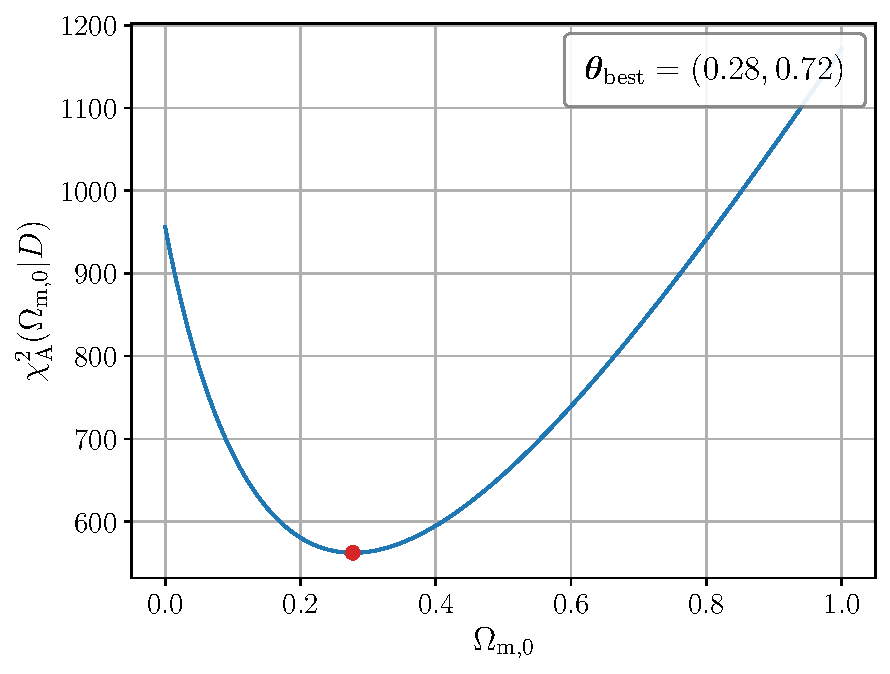
\includegraphics[scale=0.52]{figures/plots/PDF/MWE-analytic-chi2.pdf}
        \caption{Density parameter $\Omega_{\text{m},0}$ vs.\ analytically computed $\chi_{\text{A}}^2(\Omega_{\text{m},0} \vert D)$.}
        \label{fig:MWE-analytic-chi2}
    \end{minipage}
    \hspace*{1cm}
    \begin{minipage}{8cm}
        \centering
        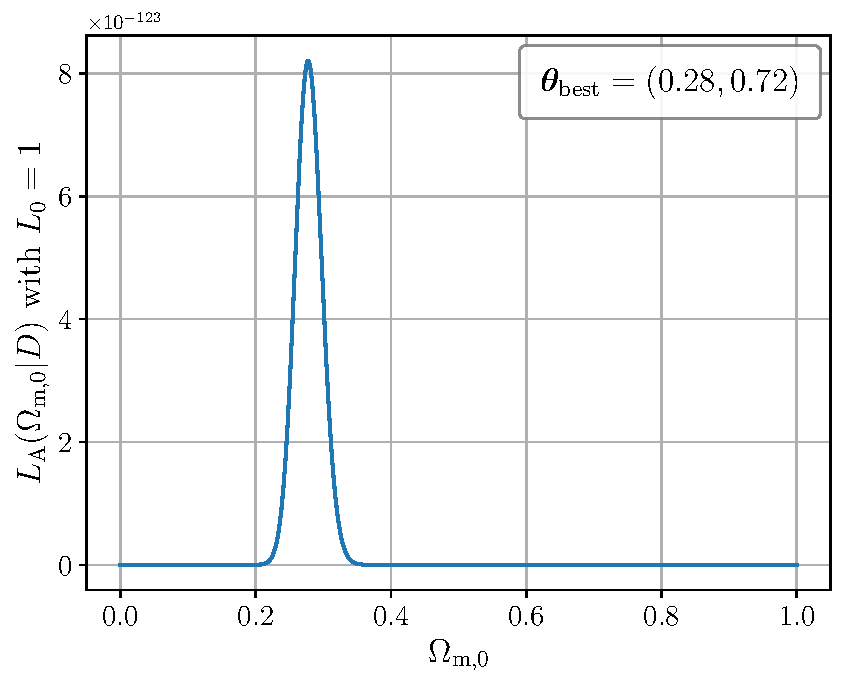
\includegraphics[scale=0.52]{figures/plots/PDF/MWE-analytic-likelihood_L0_1.pdf}
        \caption{Density parameter $\Omega_{\text{m},0}$ vs.\ likelihood $L_{\text{A}}(\Omega_{\text{m},0} \vert D)$ with $L_{0} = 1$.}
        \label{fig:MWE-analytic-likelihood-L0-1}
    \end{minipage}
\end{figure}


\noindent Before calculating the marginalized likelihood $L_{\text{M}}(\Omega_{\text{m},0} \vert D)$, let us compute the likelihood \\
$L(\mathcal{M}, \Omega_{\text{m},0} \vert D)$ (see Equation \ref{eq:likelihood}). To do so, we implement the $\chi^2$-distribution according to Equation \ref{eq:chi-square} as in Listing \ref{lst:chi-square}. Since we call \colorbox{backcolor}{\lstinline{mod_luminosity_distance}} which uses \colorbox{backcolor}{\lstinline{integral}} and therefore \colorbox{backcolor}{\lstinline{quad}}, we split the computation of the likelihood in a function \colorbox{backcolor}{\lstinline{l}} which we can provide with \colorbox{backcolor}{\lstinline{@njit}} and another function \colorbox{backcolor}{\lstinline{likelihood}} in which we compute the luminosity distance $\mathcal{D}_{\text{L}}$. 

\begin{lstlisting}[language=Python, caption={Function for $\chi^2(\mathcal{M}, \Omega_{\text{m},0} \vert D)$.}, label={lst:chi-square}]
@njit
def chi_square(magnitudes, error_magnitudes, theoretical_magnitudes):
    return np.sum(np.square((theoretical_magnitudes - magnitudes) / error_magnitudes))

\end{lstlisting}

\begin{lstlisting}[language=Python, caption={Functions for the likelihood $L(\mathcal{M}, \Omega_{\text{m},0} \vert D)$.}, label={lst:likelihood}]
@njit
def l(mod_absolute_magnitude, mod_luminosity_distance, magnitudes, error_magnitudes, L0):
    m_th = theoretical_magnitude(mod_absolute_magnitude, mod_luminosity_distance)
    chi_2 = chi_square(magnitudes, error_magnitudes, m_th)
    return L0 * np.exp(-0.5 * chi_2)


def likelihood(mod_absolute_magnitude, Omega_m0, redshifts, magnitudes, error_magnitudes, L0):
    D_L = mod_luminosity_distance(redshifts, Omega_m0)
    L = l(mod_absolute_magnitude, D_L, magnitudes, error_magnitudes, L0)
    return L
\end{lstlisting}

\noindent For calculating the marginalized likelihood $L_{\text{M}}$, we integrate over all theoretically possible values of $\mathcal{M} \in (-\infty, \infty)$ (see Equation \ref{eq:marginalized-likelihood}). Numerically, we integrate over an interval in which $L(\mathcal{M}, \Omega_{\text{m},0} \vert D)$ does no longer change significantly as a function of $\mathcal{M}$. As we see from the computation of the likelihood $L(\mathcal{M}, \Omega_{\text{m},0} \vert D)$ (see Figure \ref{fig:MWE-likelihood_mod-absolute-magnitude-vs-likelihood-at-Omega-m0-best} and \ref{fig:MWE-likelihood_mod-absolute-magnitude-vs-Omega-m0-vs-likelihood}), the relevant interval can be chosen as $\mathcal{I}_{\mathcal{M}} = [15.7, 15.9]$. 

\begin{figure}
    \begin{minipage}{8cm}
        \centering
        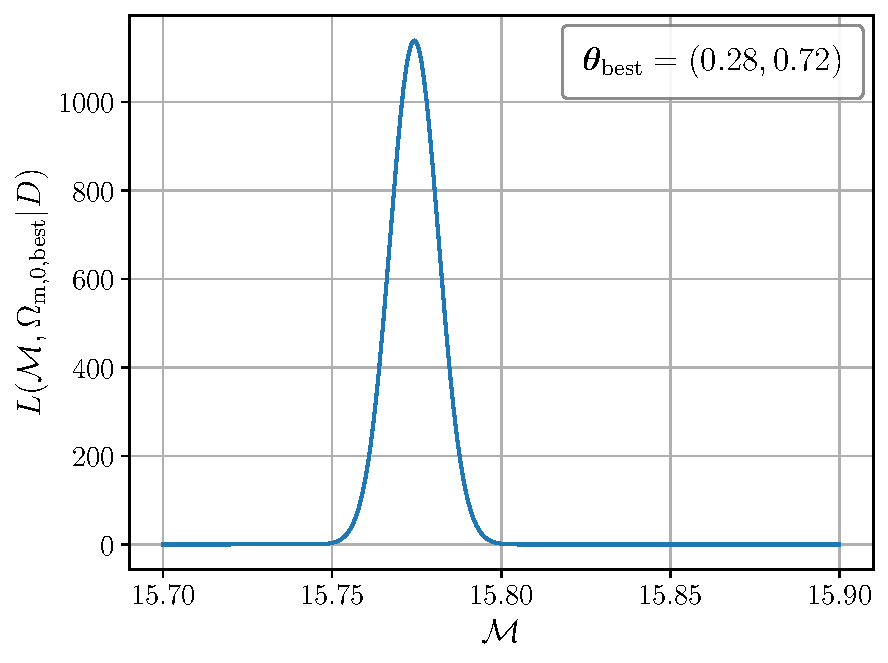
\includegraphics[scale=0.55]{figures/plots/PDF/MWE-likelihood_mod-absolute-magnitude-vs-likelihood-at-Omega-m0-best.pdf}
        \caption{Modified magnitude $\mathcal{M}$ vs.\ likelihood $L(\mathcal{M}, \Omega_{\text{m}, 0, \text{best}} \vert D)$ at $\Omega_{\text{m}, 0, \text{best}} = 0.28$.}
        \label{fig:MWE-likelihood_mod-absolute-magnitude-vs-likelihood-at-Omega-m0-best}
    \end{minipage}
    \hspace*{1cm}
    \begin{minipage}{8cm}
        \centering
        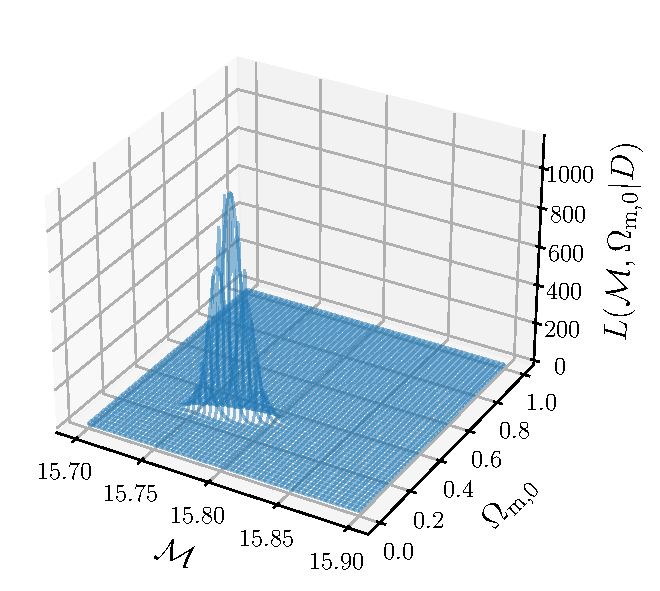
\includegraphics[scale=0.66]{figures/plots/PDF/MWE-likelihood_mod-absolute-magnitude-vs-Omega-m0-vs-likelihood.pdf}
        \caption{Modified magnitude $\mathcal{M}$ vs.\ density parameter $\Omega_{\text{m},0}$ vs.\ likelihood $L(\mathcal{M}, \Omega_{\text{m},0} \vert D)$.}
        \label{fig:MWE-likelihood_mod-absolute-magnitude-vs-Omega-m0-vs-likelihood}
    \end{minipage}
\end{figure}

\noindent The marginalized likelihood $L_{\text{M}}(\Omega_{\text{m},0} \vert D)$ can then be computed as in Listing \ref{lst:marginalized-likelihood}.

\begin{lstlisting}[language=Python, caption={Function for the marginalized likelihood $L_{\text{M}}(\Omega_{\text{m},0} \vert D)$.}, label={lst:marginalized-likelihood}]
def marginalized_likelihood(Omega_m0, redshifts, magnitudes, error_magnitudes, L0):
    D_L = mod_luminosity_distance(redshifts, Omega_m0)
    min_mod_absolute_magnitude = 15.7
    max_mod_absolute_magnitude = 15.9
    margin_L = quad(l, min_mod_absolute_magnitude, max_mod_absolute_magnitude, args=(D_L, magnitudes, error_magnitudes, L0))[0]
    return margin_L
\end{lstlisting}

\begin{figure}[H]
    \begin{minipage}{8cm}
        \centering
        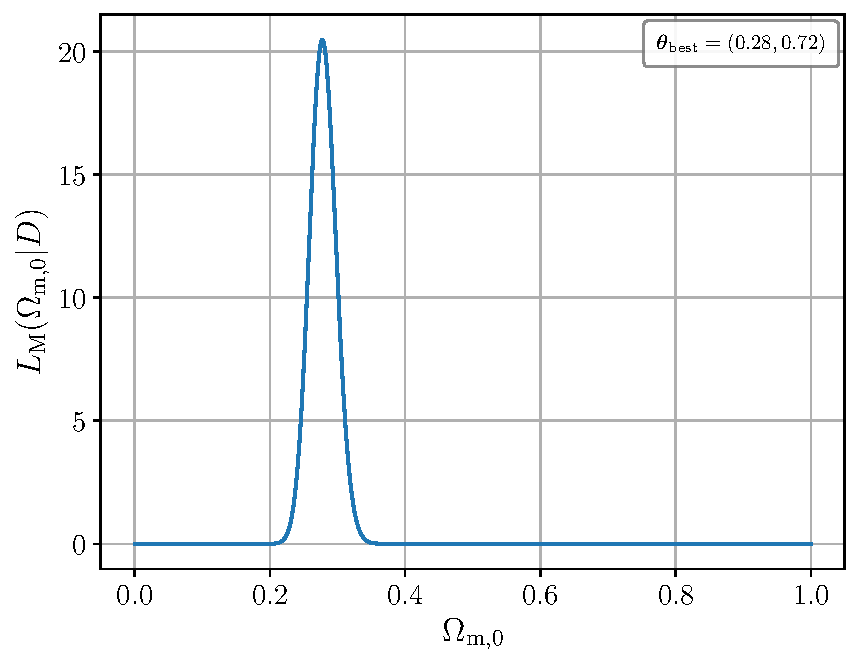
\includegraphics[scale=0.52]{figures/plots/PDF/MWE-marginalized-likelihood.pdf}
        \caption{Density parameter $\Omega_{\text{m},0}$ vs.\ marginalized likelihood $L_{\text{M}}(\Omega_{\text{m},0} \vert D)$.}
        \label{fig:MWE-marginalized-likelihood}
    \end{minipage}
    \hspace*{1cm}
    \begin{minipage}{8cm}
        \centering
        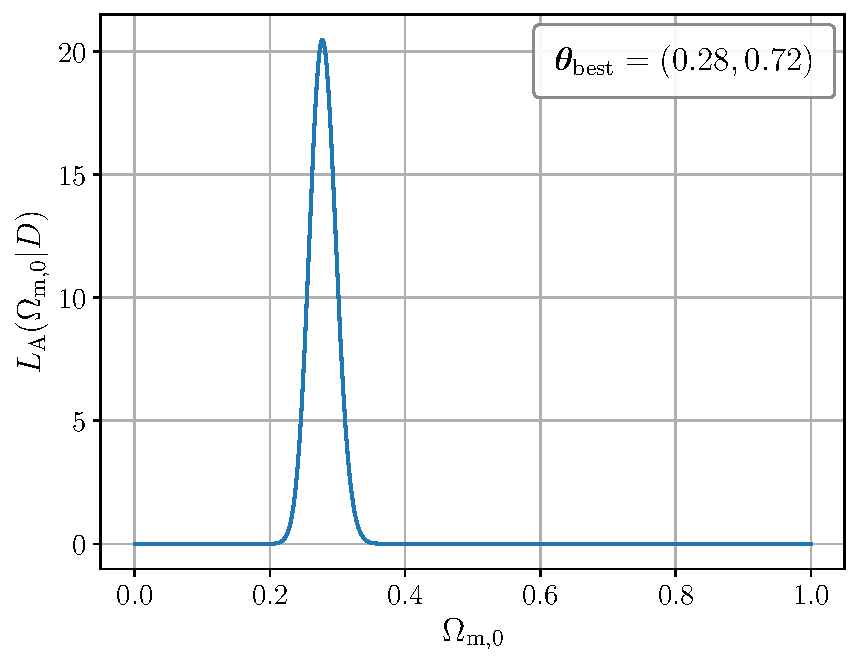
\includegraphics[scale=0.52]{figures/plots/PDF/MWE-analytic-likelihood.pdf}
        \caption{Density parameter $\Omega_{\text{m},0}$ vs.\ analytic likelihood $L_{\text{A}}(\Omega_{\text{m},0} \vert D)$.}
        \label{fig:MWE-analytic-likelihood}
    \end{minipage}
\end{figure}

\noindent As we compare the results for the marginalized likelihood $L_{\text{M}}(\Omega_{\text{m}, 0} \vert D)$ and the analytic likelihood $L_{\text{A}}(\Omega_{\text{m}, 0} \vert D)$ in the Figures \ref{fig:MWE-marginalized-likelihood} and \ref{fig:MWE-analytic-likelihood}, we see that both likelihoods are the same and lead to the same values for the parameter estimation $\vb*{\theta}_{\text{best}} = (\Omega_{\text{m}, 0, \text{best}}, \Omega_{\Lambda, 0, \text{best}}) = (0.28, 0.72)$ (rounded to two decimal places), as we have expected.

\noindent Nevertheless, the sharp pulse shape of the likelihood could lead to incorrect integration as mentioned in the \colorbox{backcolor}{\lstinline{quad}}-documentation, since the size of the function that is integrated compared to the integration interval is important to compute correct values. Therefore, we are going to calculate the $\chi^{2}$-distribution analytically for the evaluation of the $\Lambda$CDM-model in the case of an arbitrary curvature parameter $\Omega_{k,0}$ and for the valuation of the DGP-model.


\subsubsection{$\Lambda$CDM-Model with an Arbitrary Curvature Parameter $\Omega_{k,0}$}

By allowing an arbitrary curvature parameter $\Omega_{k,0} = 1 - \Omega_{\text{m},0} - \Omega_{\Lambda,0}$, the expansion function is given by 
\begin{align}
    E(z) = \sqrt{\Omega_{\text{m}, 0} (1 + z)^3 + (1 - \Omega_{\text{m},0} - \Omega_{\Lambda,0})(1 + z)^2 + \Omega_{\Lambda,0}}. \label{eq:expansion-function-arbitrary-curvature} 
\end{align}

\noindent Further, we need to take the cases of $\Omega_{k,0} < 0$ and $\Omega_{k,0} > 0$ into account when computing the (modified) luminosity distance $\mathcal{D}_{\text{L}}(z, \Omega_{\text{m},0}, \Omega_{\Lambda,0})$ (see Equations \eqref{eq:comoving-distance}, \eqref{eq:expansion-integral}, \eqref{eq:luminosity-distance} and \eqref{eq:relative-magnitude_mod-magnitude_mod-luminosity-distance}). 
First, let us have a look at the computed results for the analytically calculated $\chi^2$-distribution (see Listing \ref{lst:MWE-theoretical-magnitude-and-analytic-chi-square-and-analytic-likelihood}).

\begin{figure}[H]
    \centering
    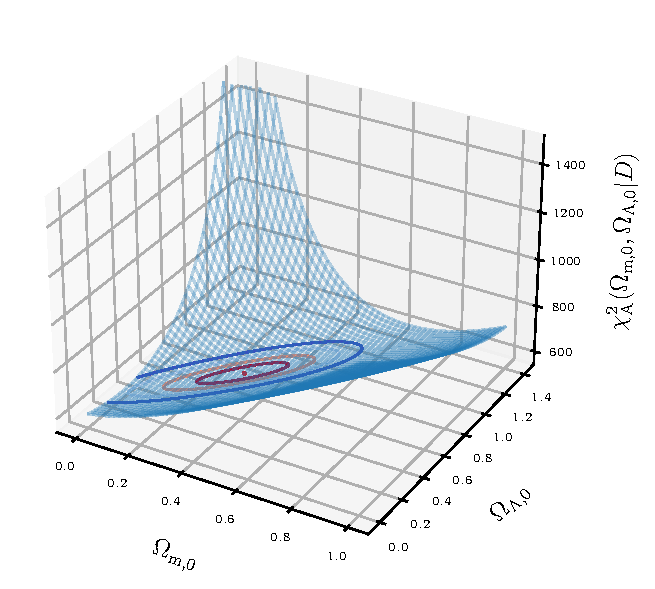
\includegraphics[scale=1.3]{figures/plots/PDF/Lambda-CDM-analytic-chi2_Omega-m0-vs-Omega-Lambda0-vs-chi2.pdf}
    \caption{Density parameters $\Omega_{\text{m},0}$ vs.\ $\Omega_{\Lambda,0}$ vs.\ analytic $\chi_{\text{A}}^2(\Omega_{\text{m},0}, \Omega_{\Lambda,0} \vert D)$.}
    \label{fig:Lambda-CDM-analytic-chi2_Omega-m0-vs-Omega-Lambda0-vs-chi2}
\end{figure}


\begin{figure}
    \begin{minipage}{8cm}
        \centering
        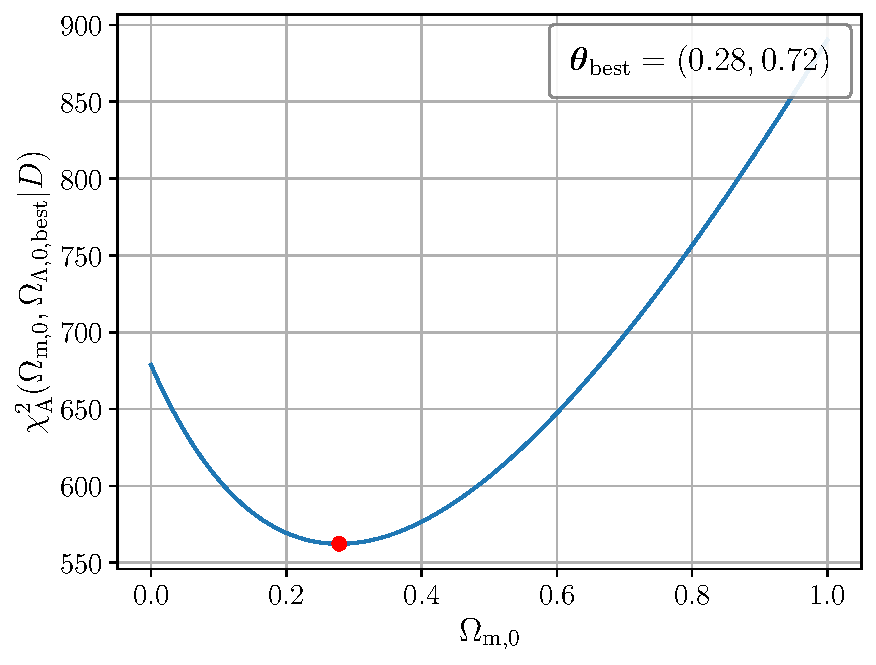
\includegraphics[scale=0.52]{figures/plots/PDF/Lambda-CDM-analytic-chi2_Omega-m0-vs-chi2-at-Omega-Lambda0-best.pdf}
        \caption{Density parameter $\Omega_{\text{m},0}$ vs.\ analytic $\chi_{\text{A}}^2(\Omega_{\text{m},0}, \Omega_{\Lambda, 0, \text{best}} \vert D)$ at $\Omega_{\Lambda, 0, \text{best}} = 0.72$.}
        \label{fig:Lambda-CDM-analytic-chi2_Omega-m0-vs-chi2-at-Omega-Lambda0-best}
    \end{minipage}
    \hspace*{1cm}
    \begin{minipage}{8cm}
        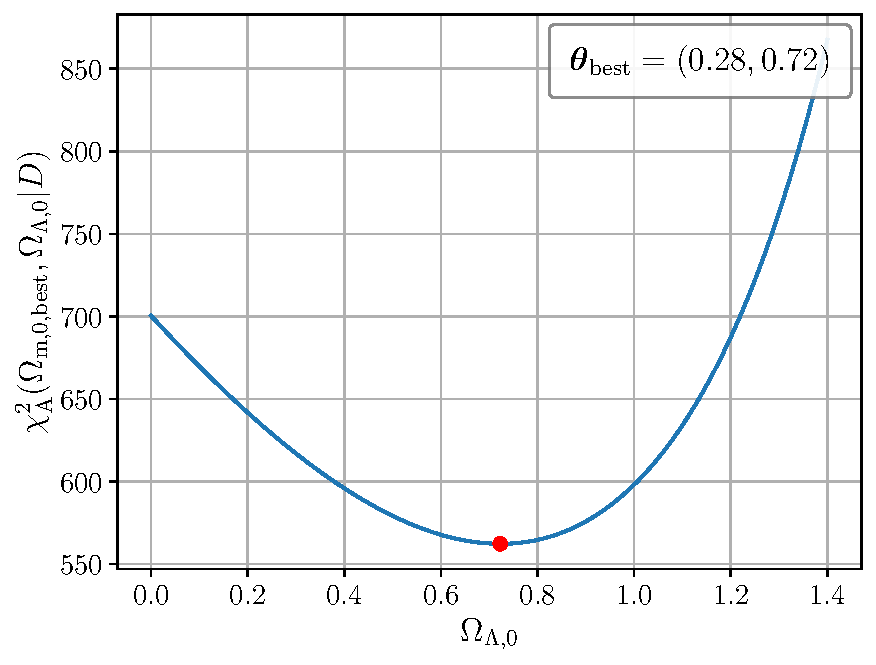
\includegraphics[scale=0.52]{figures/plots/PDF/Lambda-CDM-analytic-chi2_Omega-Lambda0-vs-chi2-at-Omega-m0-best.pdf}
        \caption{Density parameter $\Omega_{\Lambda,0}$ vs.\ analytic $\chi_{\text{A}}^2(\Omega_{\text{m}, 0, \text{best}}, \Omega_{\Lambda, 0} \vert D)$ at $\Omega_{\text{m}, 0, \text{best}} = 0.28$.}
        \label{fig:Lambda-CDM-analytic-chi2_Omega-Lambda0-vs-chi2-at-Omega-m0-best}
    \end{minipage}
\end{figure}

\noindent We obtain for the best-fit values of the $\Lambda$CDM-model with an arbitrary curvature \\
${\vb*{\theta}_{\text{best}} = (\Omega_{\text{m}, 0, \text{best}}, \Omega_{\Lambda, 0, \text{best}}) = (0.28, 0.72)}$.

\begin{figure}[H]
    \centering
    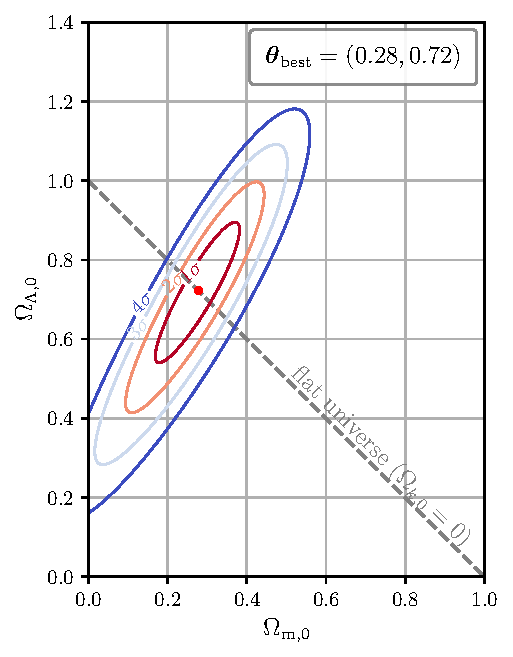
\includegraphics[scale=1.25]{figures/plots/PDF/Lambda-CDM-analytic-chi2_Omega-m0-vs-Omega-Lambda0.pdf}
    \caption{Density parameters $\Omega_{\text{m},0}$ vs.\ $\Omega_{\Lambda,0}$ with calculated $\sigma_{\vb*{\theta}}$-regions by computing $\chi_{\text{A}}^2(\Omega_{\text{m},0}, \Omega_{\Lambda,0} \vert D)$.}
    \label{fig:Lambda-CDM-analytic-chi2_Omega-m0-vs-Omega-Lambda0}
\end{figure}

\noindent To calculate $\sigma$-values for the \text{individual} parameters, we sum the (analytic) likelihood calculated for discrete values of $\vb*{\theta} \in \mathcal{I}_{\vb*{\theta}, n} = [\vb*{\theta}_{\text{min}}, \vb*{\theta}_{\text{max}}, n]$ where $n$ is the amount of linear spaced points between $\vb*{\theta}_{\text{min}}$ and $\vb*{\theta}_{\text{max}}$ such that the dependency of the likelihood $L_{\text{A}} (\vb*{\theta} \vert D)$ is reduced to one parameter. We denote
\begin{align}
    L_{\text{A}, \sum \Omega_{\Lambda,0}}(\Omega_{\text{m}, 0} \vert D) &:= \sum_{\Omega_{\Lambda, 0} \in \mathcal{I}_{\Omega_{\Lambda,0}, n}} L_{\text{A}}(\Omega_{\text{m}, 0}, \Omega_{\Lambda,0} \vert D), \\
    L_{\text{A}, \sum \Omega_{\text{m},0}} (\Omega_{\Lambda, 0} \vert D) &:= \sum_{\Omega_{\text{m}, 0} \in \mathcal{I}_{\Omega_{\text{m},0}, n}} L_{\text{A}}(\Omega_{\text{m}, 0}, \Omega_{\Lambda,0} \vert D)
\end{align}
This to one parameter reduced likelihood has the shape of a (one dimensional) Gaussian curve. Its standard deviation is considered as the $\sigma$-value for the individual parameter. \\
We obtain this $\sigma$-value by fitting a Gaussian curve with \colorbox{backcolor}{\lstinline{scipy.optimize.curve_fit}}\footnote{Documentation of \colorbox{backcolor}{\lstinline{scipy.optimize}}-package: \href{https://docs.scipy.org/doc/scipy/reference/optimize.html}{https://docs.scipy.org/doc/scipy/reference/optimize.html}} for the computed, reduced likelihood.

\begin{figure}[H]
    \centering
    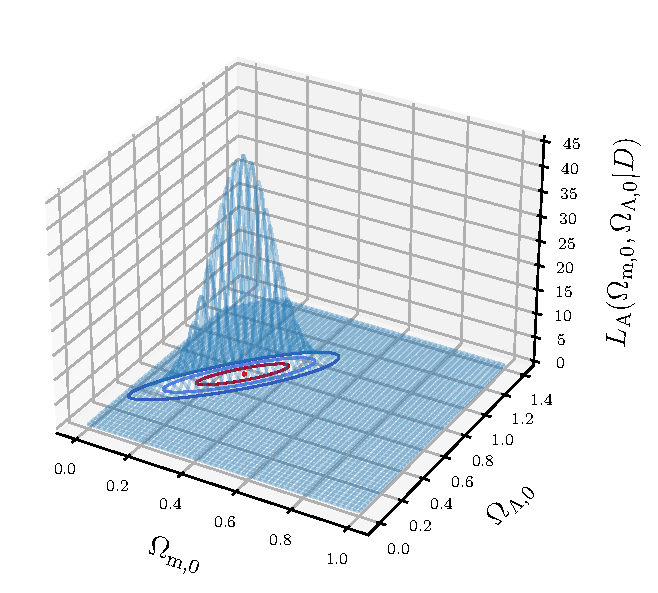
\includegraphics[scale=0.72]{figures/plots/PDF/Lambda-CDM-analytic-likelihood_Omega-m0-vs-Omega-Lambda0-vs-likelihood.pdf}
    \caption{Density parameters $\Omega_{\text{m},0}$ vs.\ $\Omega_{\Lambda,0}$ vs.\ analytic likelihood $L_{\text{A}}(\Omega_{\text{m},0}, \Omega_{\Lambda,0} \vert D)$.}
    \label{fig:Lambda-CDM-analytic-likelihood_Omega-m0-vs-Omega-Lambda0-vs-likelihood}
\end{figure}


\begin{figure}[H]
   \begin{minipage}{8cm}
      \centering
      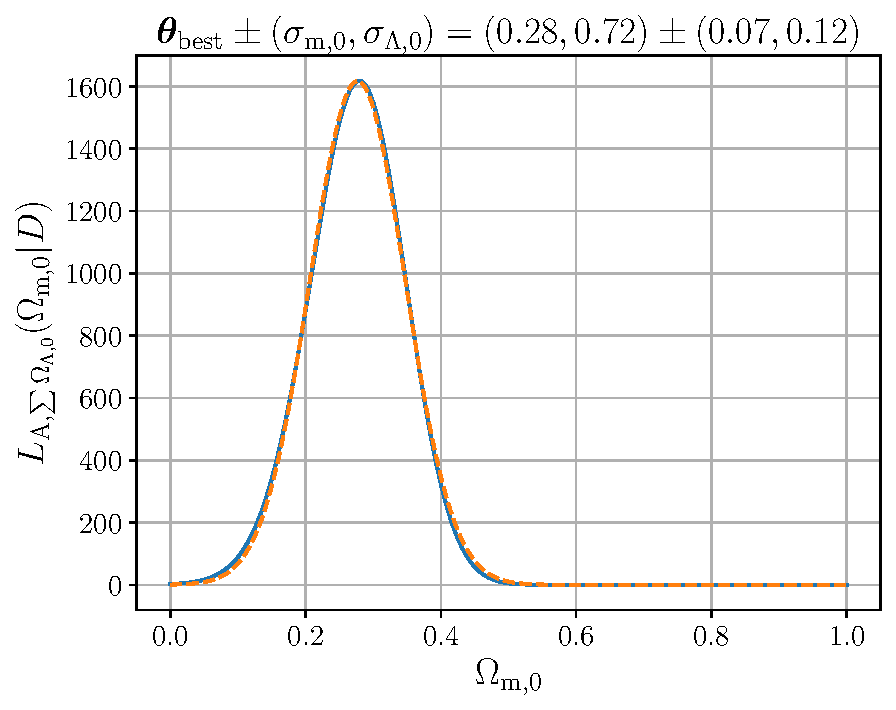
\includegraphics[scale=0.52]{figures/plots/PDF/Lambda-CDM-analytic-likelihood_Omega-m0-vs-likelihood-summed-Omega-Lambda0.pdf}
      \caption{Density parameters $\Omega_{\text{m},0}$ vs.\ reduced, analytic likelihood $L_{\text{A}, \sum \Omega_{\Lambda,0}}(\Omega_{\text{m},0} \vert D)$ and its fit.}
      \label{fig:Lambda-CDM-analytic-likelihood_Omega-m0-vs-likelihood-summed-Omega-Lambda0}
   \end{minipage}
   \hspace*{1cm}
   \begin{minipage}{8cm}
      \centering
      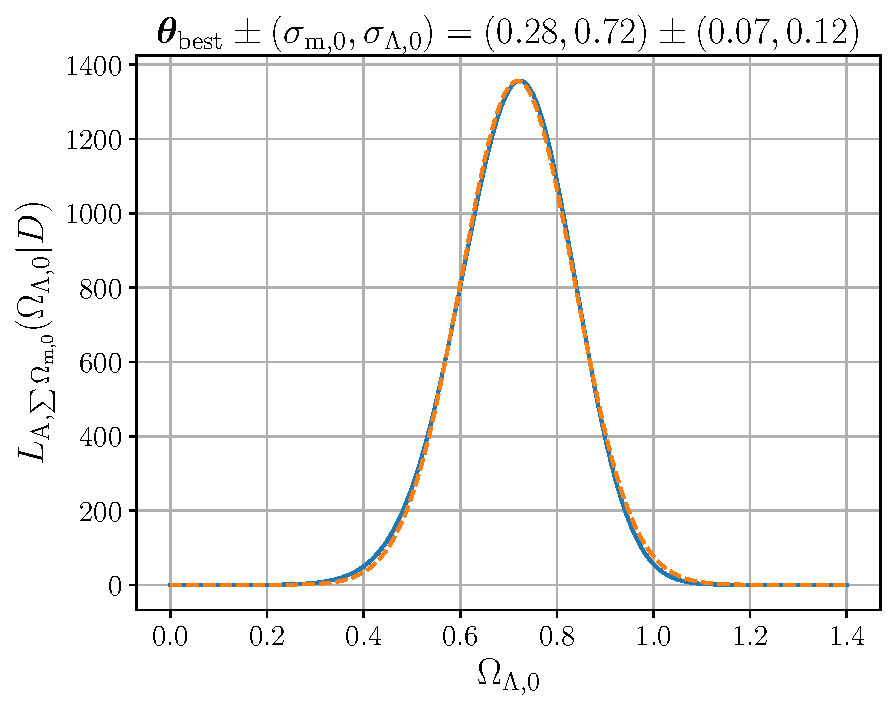
\includegraphics[scale=0.52]{figures/plots/PDF/Lambda-CDM-analytic-likelihood_Omega-Lambda0-vs-likelihood-summed-Omega-m0.pdf}
      \caption{Density parameters $\Omega_{\Lambda,0}$ vs.\ reduced, analytic likelihood $L_{\text{A}, \sum \Omega_{\text{m},0}}(\Omega_{\Lambda,0} \vert D)$ and its fit.}
      \label{fig:Lambda-CDM-analytic-likelihood_Omega-Lambda0-vs-likelihood-summed-Omega-m0}
   \end{minipage}
\end{figure}

\begin{figure}[H]
    \begin{minipage}{8cm}
       \centering
       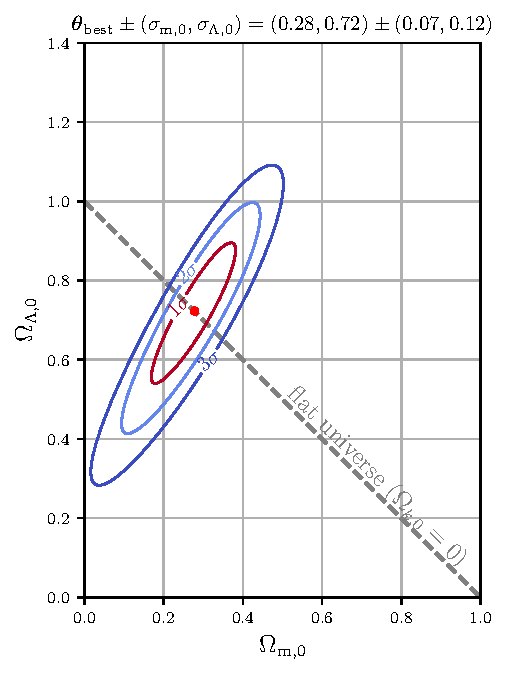
\includegraphics[scale=1.0]{figures/plots/PDF/Lambda-CDM-analytic-likelihood_Omega-m0-vs-Omega-Lambda0.pdf}
       \caption{Density parameters $\Omega_{\text{m},0}$ vs.\ $\Omega_{\Lambda,0}$ with calculated $\sigma_{\vb*{\theta}}$-regions by computing the analytic likelihood $L_{\text{A}}(\Omega_{\text{m},0}, 
       \Omega_{\Lambda,0} \vert D)$.}
       \label{fig:Lambda-CDM-analytic-likelihood_Omega-m0-vs-Omega-Lambda0}
    \end{minipage}
    \hspace*{1cm}
    \begin{minipage}{8cm}
       \centering
       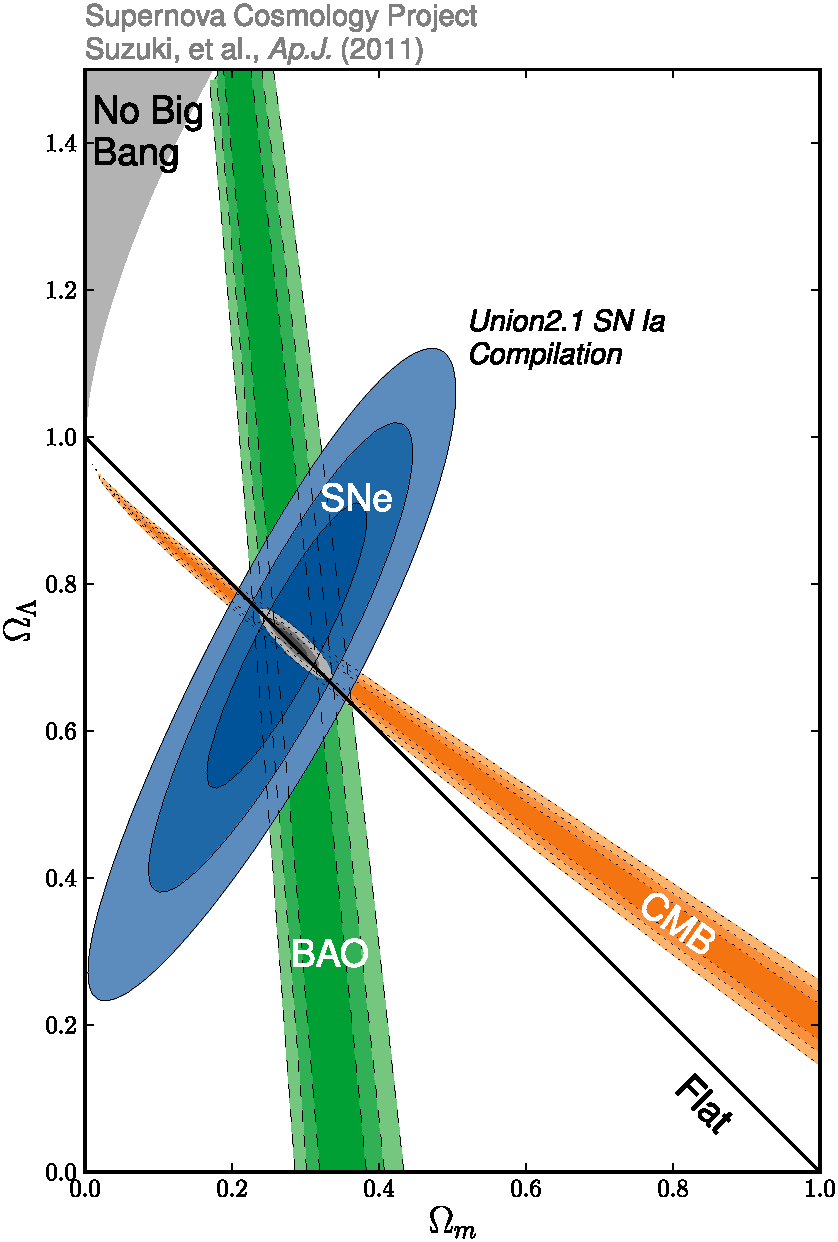
\includegraphics[scale=0.53]{figures/plots/PDF/Union2.1_Om-Ol_slide.pdf}
       \caption{Density parameters $\Omega_{\text{m},0}$ vs.\ $\Omega_{\Lambda,0}$ with calculated $\sigma_{\vb*{\theta}}$-regions by the \textit{Supernova Cosmology Project}. \\
       Source: \cite[Figure 5]{Suzuki2012}}
       \label{fig:Union2.1_Om-Ol_slide}
    \end{minipage}
\end{figure}

\noindent Finally, we can specify the best-fit values with errors as
$\vb*{\theta}_{\text{best}} \pm (\sigma_{\text{m},0}, \sigma_{\Lambda,0}) = (0.28, 0.72) \pm (0.07, 0.12)$. As we compare Figures \ref{fig:Lambda-CDM-analytic-likelihood_Omega-m0-vs-Omega-Lambda0} and \ref{fig:Union2.1_Om-Ol_slide}, we can conclude that our method and code (see appendix \ref{app:dataset-and-source-codes}) can reproduce the results by the \textit{Supernovae Cosmology Project}, though the calculated errors for the individual parameters are slightly larger in our case. \\ 
By considering further constraints like measurements of the cosmic microwave background (CMB) or baryonic acoustic oscillations (BAO), it is possible to specify the best-fit values more precisely and reduce their uncertainty significantly (see \cite[Table 7]{Suzuki2012} and \cite[Table 6 and 7]{Planck2020}).


\subsection{DGP-Model}

For the DGP-model, we implement the modified Friedmann Equations (see Equation \ref{eq:dgp-friedmann-interpolation}) and its derivative with respect to $z$ assuming $z = \text{const.}$ as in Listing \ref{lst:dgp-friedmann-interpolation}. 
\begin{lstlisting}[language=Python, caption={Function for modified Friedmann Equation and its derivative assuming $z = \text{const}$.}, label={lst:dgp-friedmann-interpolation}]
@njit
def mod_friedmann(E, z, Omega_m0, alpha):
    return E * E - (1.0 - Omega_m0) * np.power(E, alpha) - Omega_m0 * np.power(1.0 + z, 3)

@njit
def deriv_mod_friedmann(E, _, Omega_m0, alpha):
    return 2.0 * E - alpha * (1.0 - Omega_m0) * np.power(E, alpha - 1.0)
\end{lstlisting}

\noindent To compute the solution of the modified Friedmann Equation for $E(z)$, we use the \colorbox{backcolor}{\lstinline{root}}-function provided by \colorbox{backcolor}{\lstinline{scipy.optimize}} and implement the solution as in Listing \ref{lst:dgp-friedmann-interpolation-solution}.

\begin{lstlisting}[language=Python, caption={Function to find the solution of the modified Friedmann Equation.}, label={lst:dgp-friedmann-interpolation-solution}]
def sol_friedmann(z, Omega_m0, alpha, mod_friedmann, mod_deriv_friedmann):
    # Solves the modified friedmann equation f(z) = 0 for z with exterior derivative mod_deriv_friedmann
    return opt.root(mod_friedmann, 1.0, args=(z, Omega_m0, alpha), jac=mod_deriv_friedmann).x[0]
\end{lstlisting}

\noindent As in the $\Lambda$CDM-model, it is demanded to calculate the (modified) luminosity distance $\mathcal{D}_{\text{L}}$. Since the implemented computation of $E(z)$ as in Listing \ref{lst:dgp-friedmann-interpolation-solution} is not trivial for \colorbox{backcolor}{\lstinline{quad}} to integrate over, we interpolate the integrand by a sample of redshifts $z'$ and the expansion function $E(z')$ that solves Equation \ref{eq:dgp-friedmann-interpolation} for this sample.


\begin{lstlisting}[language=Python, caption={Functions for computation of the (modified) luminosity distance $\mathcal{D}_{\text{L}}$ in the DGP-model.}, label={lst:dgp-computation-mod-luminosity-distance}]
@njit
def interp_integrand(z, sample_redshifts, sample_E):
    if z == 0.0:
        return 1.0

    E = np.interp(z, sample_redshifts, sample_E)
    return 1.0/E

def interp_integral(z, sample_redshifts, sample_E):
    # d_C/d_H = Integrate[1/E(z'), {z', 0, z}]
    return quad(interp_integrand, 0.0, z, args=(sample_redshifts, sample_E))[0]

def mod_luminosity_distance(z, Omega_m0, alpha):
    # Cosmological Parameters
    # =======================
    c = 299792.458           # speed of light in vacuum in km/s
    H_0 = 1.0                # dependence on hubble constant is set into the mod_absolute_magnitude, see theoretical_magnitude
    d_H = c/H_0              # hubble distance
    # =======================
    
    sample_redshifts = np.linspace(0.0, max(z), 1000)
    sample_E = np.array([sol_friedmann(zi, Omega_m0, alpha, mod_friedmann, deriv_mod_friedmann) for zi in sample_redshifts])

    I = np.array([interp_integral(zi, sample_redshifts, sample_E) for zi in z])
    
    return (1.0 + z) * d_H * I
\end{lstlisting}

\noindent Further, we compute the $\chi^2$-distribution analytically as in Listing \ref{lst:MWE-theoretical-magnitude-and-analytic-chi-square-and-analytic-likelihood} and \ref{lst:dgp-chi2}. In the following, we only consider $\chi_{\text{A}}^{2}(\Omega_{\text{m,0}}, \alpha \vert D)$, which is sufficient to estimate best-fit values for $\vb*{\theta} = (\Omega_{\text{m},0}, \alpha)$.

\begin{lstlisting}[language=Python, caption={Function for analytic $\chi_{\text{A}}^2(\Omega_{\text{m},0}, \alpha \vert D)$.}, label={lst:dgp-chi2}]
def chi2(Omega_m0, alpha, redshifts, magnitudes, error_magnitudes):
    mod_absolute_magnitude = 0.0
    D_L = mod_luminosity_distance(redshifts, Omega_m0, alpha)
    m_th = theoretical_magnitude(mod_absolute_magnitude, D_L)
    chi_2 = analytic_chi_square(magnitudes, error_magnitudes, m_th)
    return chi_2  
\end{lstlisting}

\begin{figure}[]
    \begin{minipage}{8cm}
        \centering
        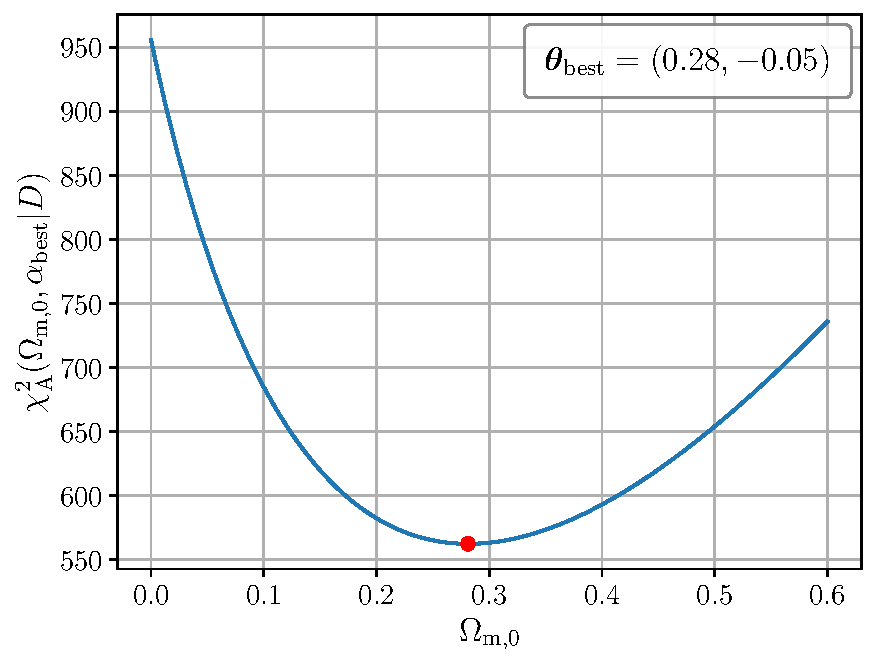
\includegraphics[scale=0.50]{figures/plots/PDF/DGP-analytic-chi2_Omega-m0-vs-chi2-at-alpha-best.pdf}
        \caption{Density parameter $\Omega_{\text{m},0}$ vs.\ analytic $\chi_{\text{A}}^2(\Omega_{\text{m},0}, \alpha_{\text{best}} \vert D)$ at $\alpha_{\text{best}} = -0.05$.}
        \label{fig:DGP-analytic-chi2_Omega-m0-vs-chi2-at-alpha-best}
    \end{minipage}
    \hspace*{0.5cm}
    \begin{minipage}{8.2cm}
       \centering
       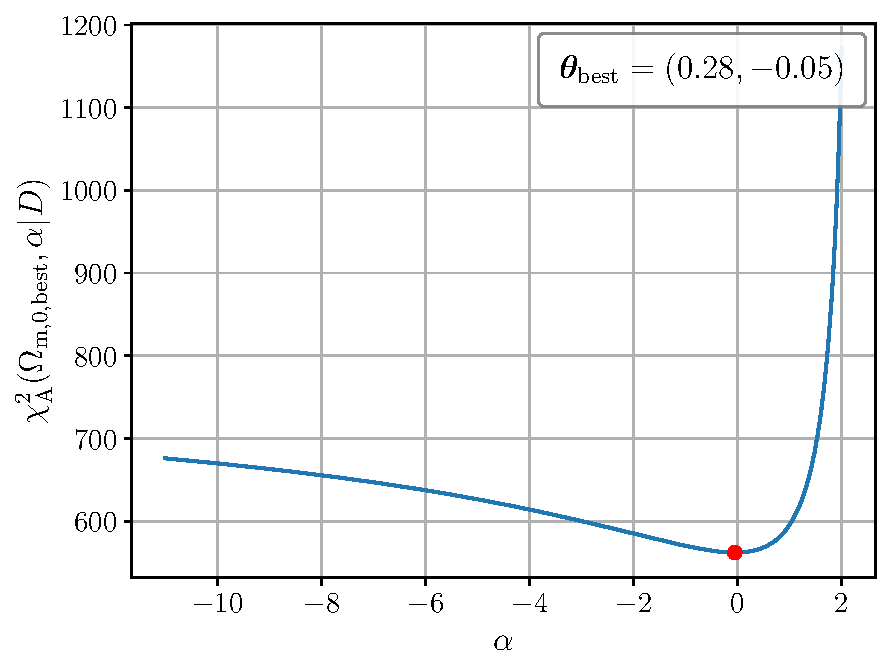
\includegraphics[scale=0.50]{figures/plots/PDF/DGP-analytic-chi2_alpha-vs-chi2-at-Omega-m0-best.pdf}
       \caption{Interpolation parameter $\alpha$ vs.\ analytic $\chi_{\text{A}}^2(\Omega_{\text{m}, 0, \text{best}}, \alpha \vert D)$ at $\Omega_{\text{m}, 0, \text{best}} = 0.28$.}
       \label{fig:DGP-analytic-chi2_alpha-vs-chi2-at-Omega-m0-best}
    \end{minipage}
\end{figure}

\begin{figure}[H]
    \centering
    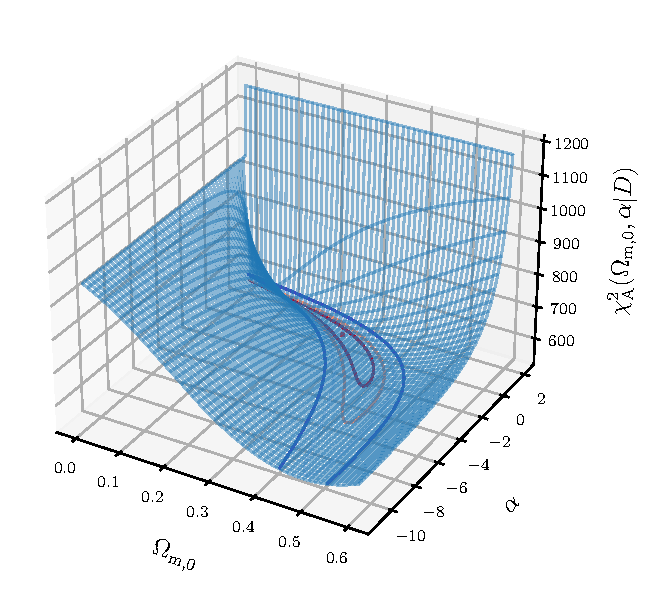
\includegraphics[scale=1.0]{figures/plots/PDF/DGP-analytic-chi2_Omega-m0-vs-alpha-vs-chi2.pdf}
    \caption{Density parameter $\Omega_{\text{m},0}$ vs.\ interpolation parameter $\alpha$ vs.\ analytic $\chi_{\text{A}}^2(\Omega_{\text{m},0}, \alpha \vert D)$.}
    \label{fig:DGP-analytic-chi2_Omega-m0-vs-alpha-vs-chi2}
\end{figure}

\noindent Finally, we obtain for the best-fit values $\vb*{\theta}_{\text{best}} = (0.28, -0.05)$. 
As we see in Figure \ref{fig:DGP-analytic-chi2_Omega-m0-vs-alpha-vs-chi2} and Figure \ref{fig:DGP-analytic-chi2_Omega-m0-vs-alpha-full}, the $\sigma_{\vb*{\theta}}$-regions spread out broadly in parameter space as the $\chi^2$-distribution flattens. This makes it difficult to give an adequate estimate of the $\sigma$-uncertainties for the individual parameters. Nevertheless, we can conclude that this parameter estimation of $\vb*{\theta} = (\Omega_{\text{m},0}, \alpha)$ tends to prefer the $\Lambda$CDM-model (for which $\alpha = 0$) over the DGP-model (for which $\alpha = 1$). As shown in Figure \ref{fig:testing-DGP-with-planck} (see \cite[Figure 3]{Li2013}), accounting multiple datasets such as measurements of baryonic acoustic oscillations (BAO) or cosmic microwave background (Planck), but also measurements of weak gravitational lensing (see \cite[Figure 7]{Thomas2009}) allow constraints that disfavour the DGP-model.

\begin{figure}[]
    \centering
    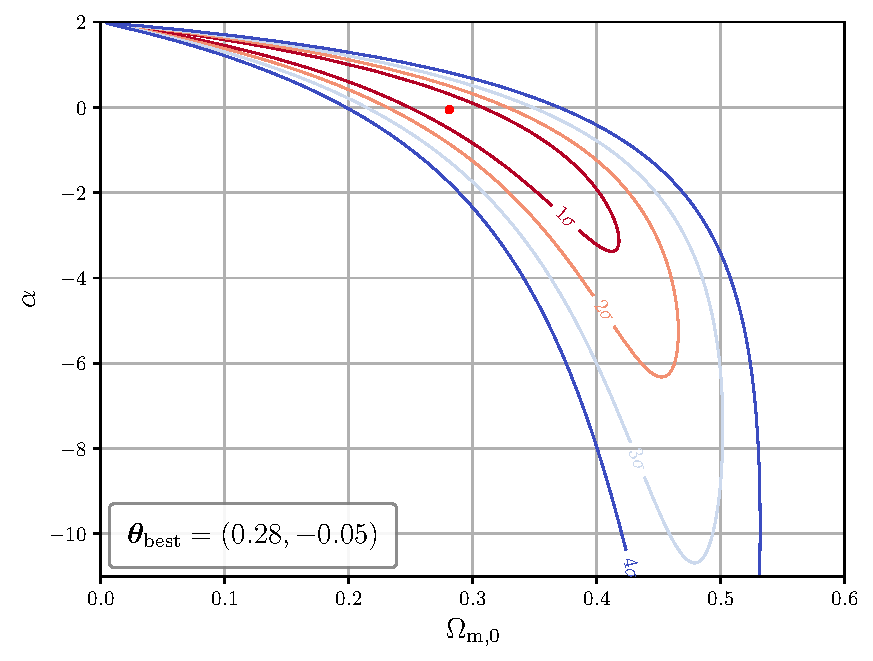
\includegraphics[scale=1.0]{figures/plots/PDF/DGP-analytic-chi2_Omega-m0-vs-alpha-full.pdf}
    \caption{Density parameter $\Omega_{\text{m},0}$ vs.\ interpolation parameter $\alpha$ with calculated $\sigma_{\vb*{\theta}}$-regions by computing $\chi_{\text{A}}^2(\Omega_{\text{m},0}, \alpha \vert D)$.}
    \label{fig:DGP-analytic-chi2_Omega-m0-vs-alpha-full}
\end{figure}

\begin{figure}
    \begin{minipage}{8cm}
        \centering
        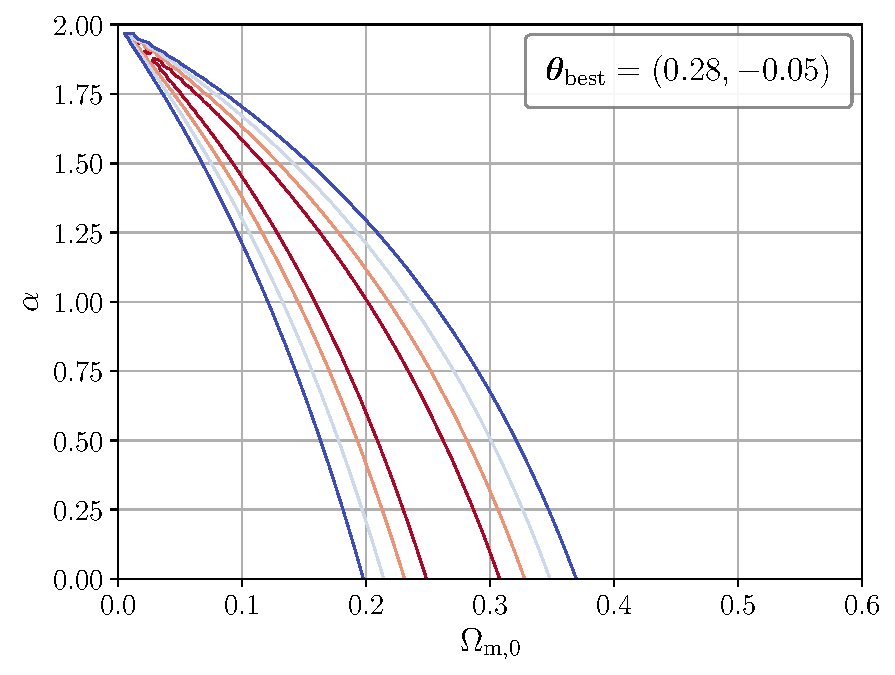
\includegraphics[scale=0.53]{figures/plots/PDF/DGP-analytic-chi2_Omega-m0-vs-alpha-0-2.pdf}
        \caption{Density parameter $\Omega_{\text{m},0}$ vs.\ interpolation parameter $\alpha$ with calculated $\sigma_{\vb*{\theta}}$-regions for $\alpha \in [0.0, 2.0]$.}
        \label{fig:DGP-analytic-chi2_Omega-m0-vs-alpha-0-2}
    \end{minipage}
    \hspace*{1cm}
    \begin{minipage}{8cm}
        \centering
        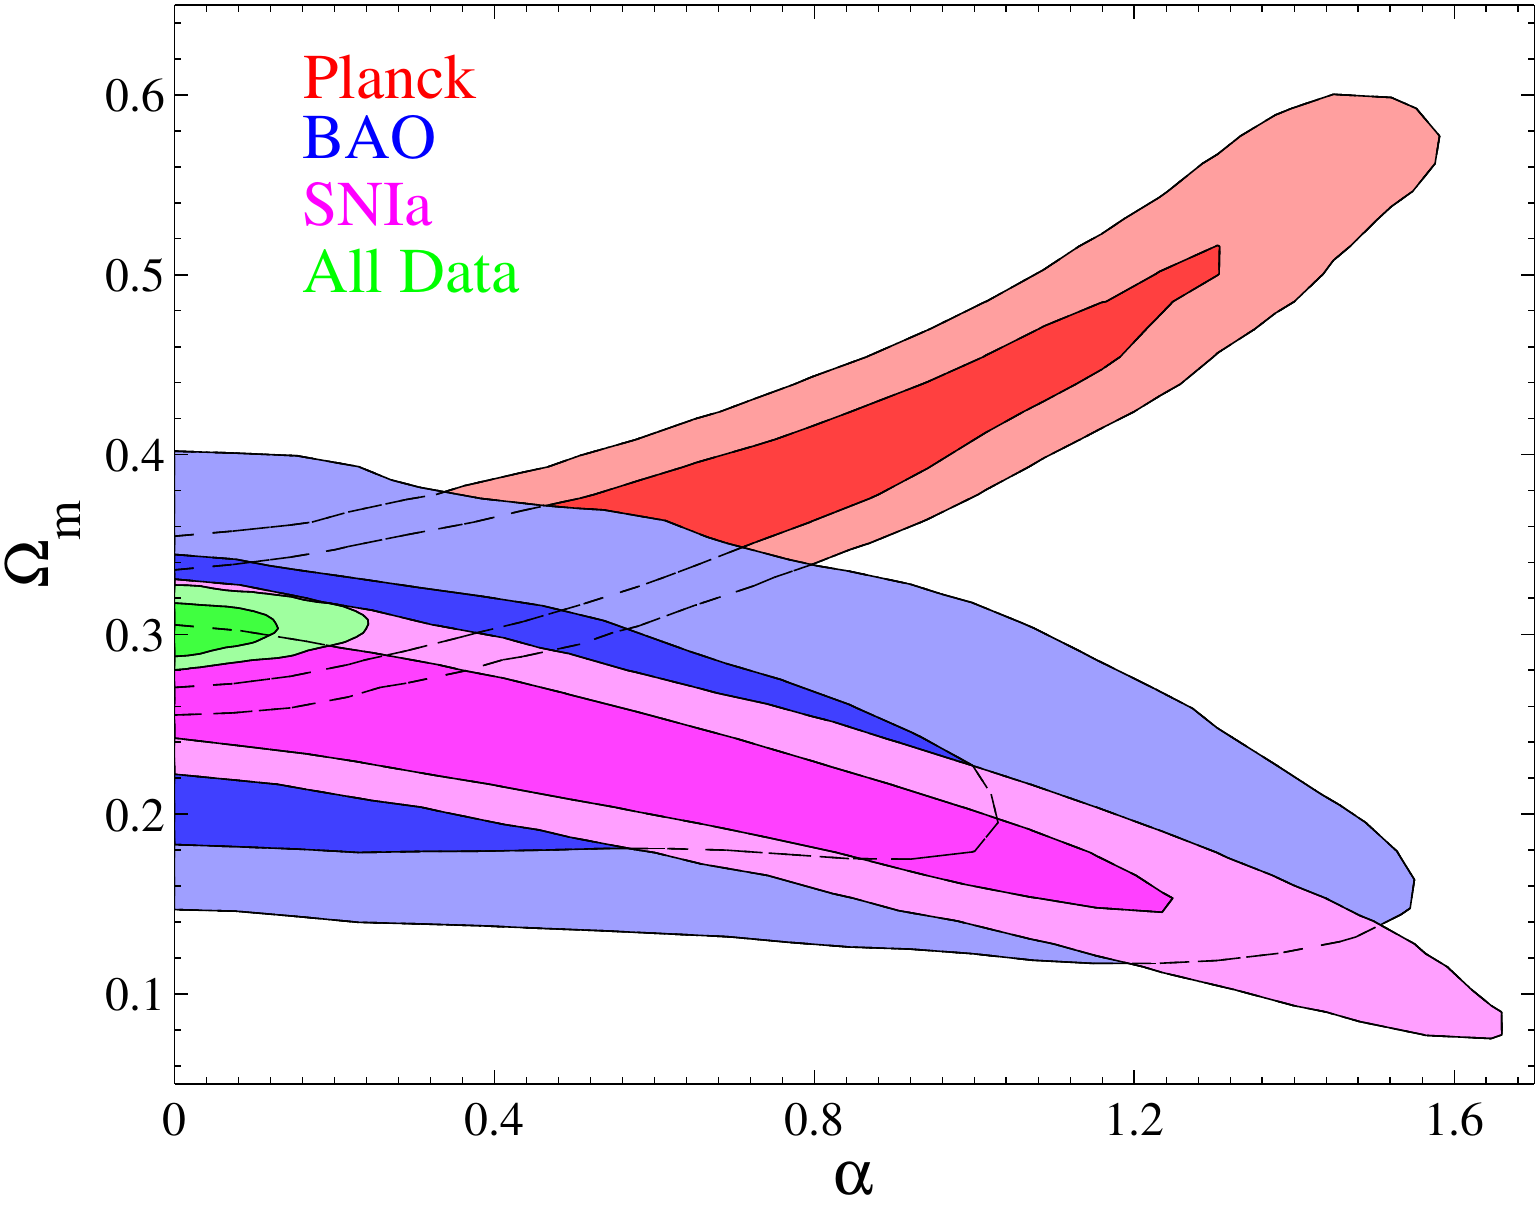
\includegraphics[scale=0.55]{figures/plots/PNG/testing-DGP-with-planck.png}
        \caption{Density parameter $\Omega_{\text{m},0}$ vs.\ interpolation parameter $\alpha$ considering several cosmological constraints. \\
        Source: \cite[Figure 3]{Li2013}}
        \label{fig:testing-DGP-with-planck} 
    \end{minipage}
\end{figure}




%%% CONCLUSION
\chapter{Conclusion}
\thispagestyle{empty}

\noindent First of all, we see that the computational implementation carried out in this thesis are able to reproduce the results of the \textit{Supernovae Cosmology Project} using the ``Union2.1'' SN Ia dataset.
Further, the result of $\Omega_{\text{m},0,\text{best}} = 0.28$ in both cases, $\vb*{\theta} = (\Omega_{\text{m},0}, \Omega_{\Lambda,0})$ and $\vb*{\theta} = (\Omega_{\text{m},0}, \alpha)$, shows consistency in the computational implementation of our parameter estimation. \\

\noindent The obtained values of $(\Omega_{\text{m}, 0, \text{best}}, \Omega_{\Lambda, 0, \text{best}}) \pm (\sigma_{\text{m}, 0}, \sigma_{\Lambda,0}) = (0.28, 0.72) \pm (0.07, 0.12)$ and \\
${(\Omega_{\text{m}, 0, \text{best}}, \alpha_{\text{best}}) = (0.28, -0.05)}$ prefer the $\Lambda$CDM-model for a flat universe. Yet, the large errors, especially in the case of analyzing the parameter pair $\vb*{\theta} = (\Omega_{\text{m},0}, \alpha)$, do not allow a final judgement on the cosmological models by using the ``Union2.1'' SN Ia dataset alone (as mentioned in \cite{Thomas2009}). This can also be seen in Figure \ref{fig:distance-modulus-vs-redshift}, where the predicted relation between distance modulus and redshift in both the $\Lambda$CDM-model and the DGP-model match even for high-redshift datapoints and therefore do not allow a clear distinction. Only under consideration of multiple measurements as the cosmic microwave background (CMB), baryonic acoustic oscillations (BAO) and weak gravitational lensing, it is possible to provide constraints that favour the $\Lambda$CDM-model and disfavour the DGP-model.

\noindent Nevertheless, the physical interpretation of the cosmological constant $\Lambda$ needs 


%%% APPENDIX
\begin{appendix}

\chapter{The first appendix}
\thispagestyle{empty}

Here is the first appendix.


\chapter{The second appendix}
\thispagestyle{empty}

Here comes the second appendix.

\end{appendix}



%%%%%%%%%%%%%%%%%%%
%%% BACK MATTER %%%
%%% =========== %%%

\backmatter

%%% BIBLIOGRAPHY
\nocite{*}
\phantomsection\addcontentsline{toc}{chapter}{Bibliography}
\printbibliography

%%% LIST OF FIGURES
% \listoffigures

%%% LIST OF TABLES
% \listoftables

% \NewPage
% \NewPage

%%% DECLARATION OF AUTHORSHIP 
\chapter*{Declaration of authorship}
\thispagestyle{empty}

I have done this all on my own -- trust me ;)


% \NewPage
% \NewPage

\end{document}
